\documentclass[12pt]{extarticle}
\usepackage[paperwidth=18in,paperheight=8.5in]{geometry}
\usepackage{amsmath}
\usepackage{hyperref}
\usepackage{multirow}
\usepackage{pdfpages}
\usepackage[utf8]{inputenc}
\title{Kaon mixing: chiral and continuum extrapolations}
\author{R Mukherjee}
\date{\today}
\begin{document}
\maketitle
\tableofcontents
\clearpage
\begin{figure}
\centering
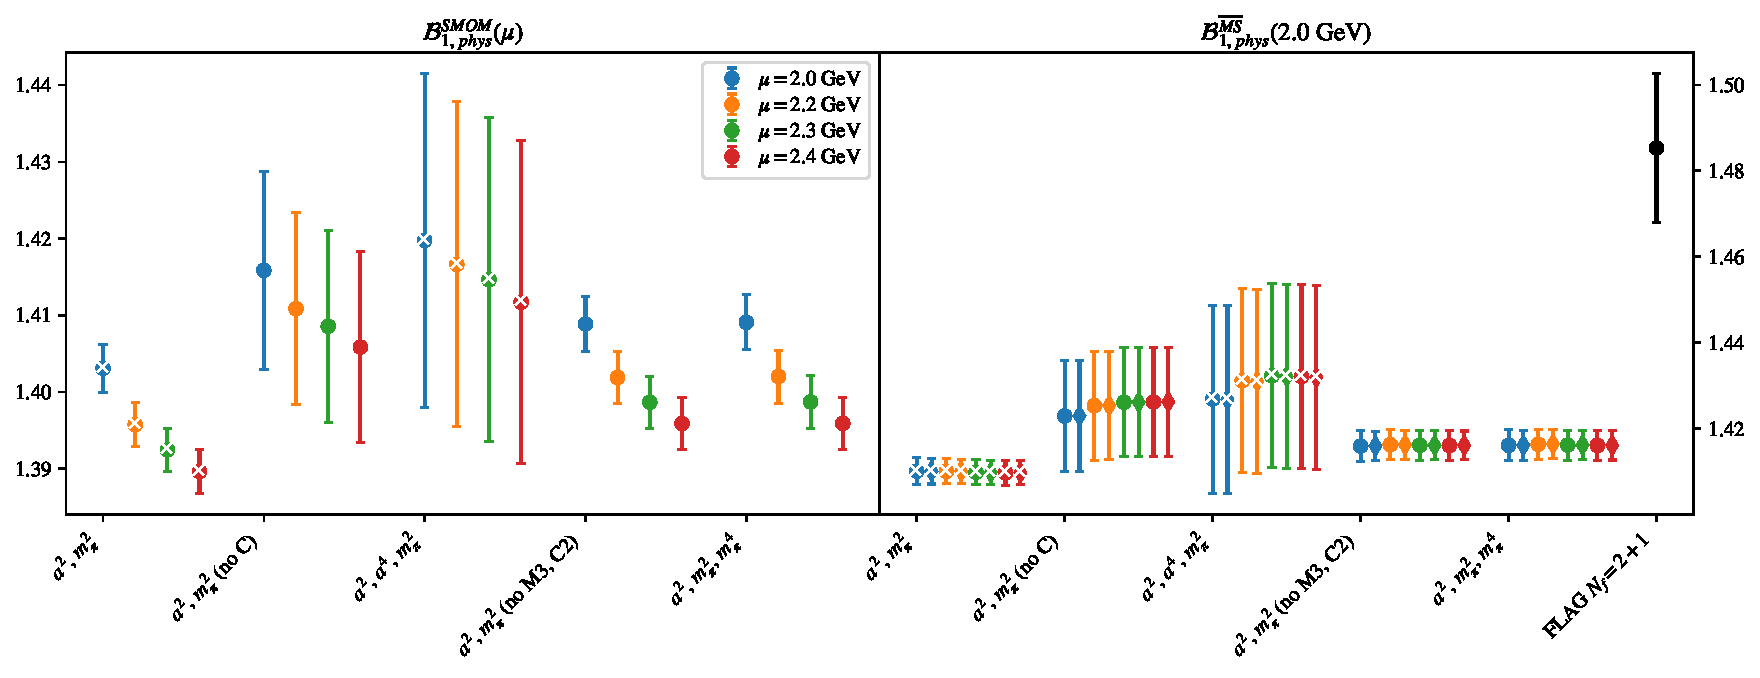
\includegraphics[page=1, width=1.1\textwidth]{VVpAA/SUSY/fit_summary_bag.pdf}
\caption{$\mathcal{B}_{1}$\\(left) $\mathcal{B}_{phys}$ in RI/SMOM scheme from fit variations (fits with $p$-value $<0.05$ marked with ``$\times$"). \\(right) $\mathcal{B}_{phys}$ in $\overline{MS}$ computed using $\mathcal{B}^{\overline{MS}} = R^{\overline{MS}\leftarrow SMOM}(2.0)\sigma_{npt}(2.0,\mu) \mathcal{B}^{SMOM}(\mu)$.}
\end{figure}
\clearpage
\begin{figure}
\centering
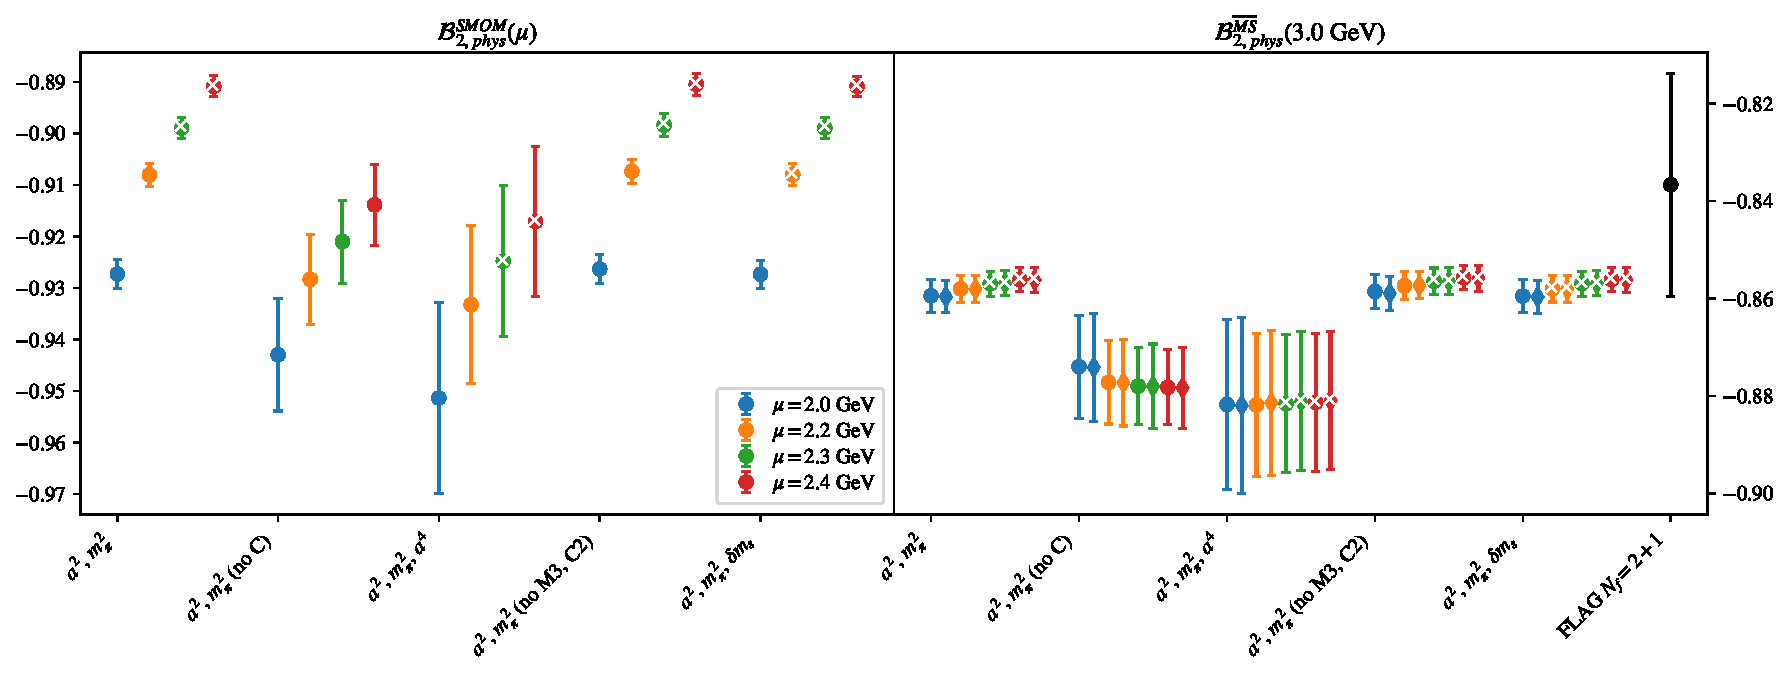
\includegraphics[page=1, width=1.1\textwidth]{VVmAA/SUSY/fit_summary_bag.pdf}
\caption{$\mathcal{B}_{2}$\\(left) $\mathcal{B}_{phys}$ in RI/SMOM scheme from fit variations (fits with $p$-value $<0.05$ marked with ``$\times$"). \\(right) $\mathcal{B}_{phys}$ in $\overline{MS}$ computed using $\mathcal{B}^{\overline{MS}} = R^{\overline{MS}\leftarrow SMOM}(3.0)\sigma_{npt}(3.0,\mu) \mathcal{B}^{SMOM}(\mu)$.}
\end{figure}
\clearpage
\begin{figure}
\centering
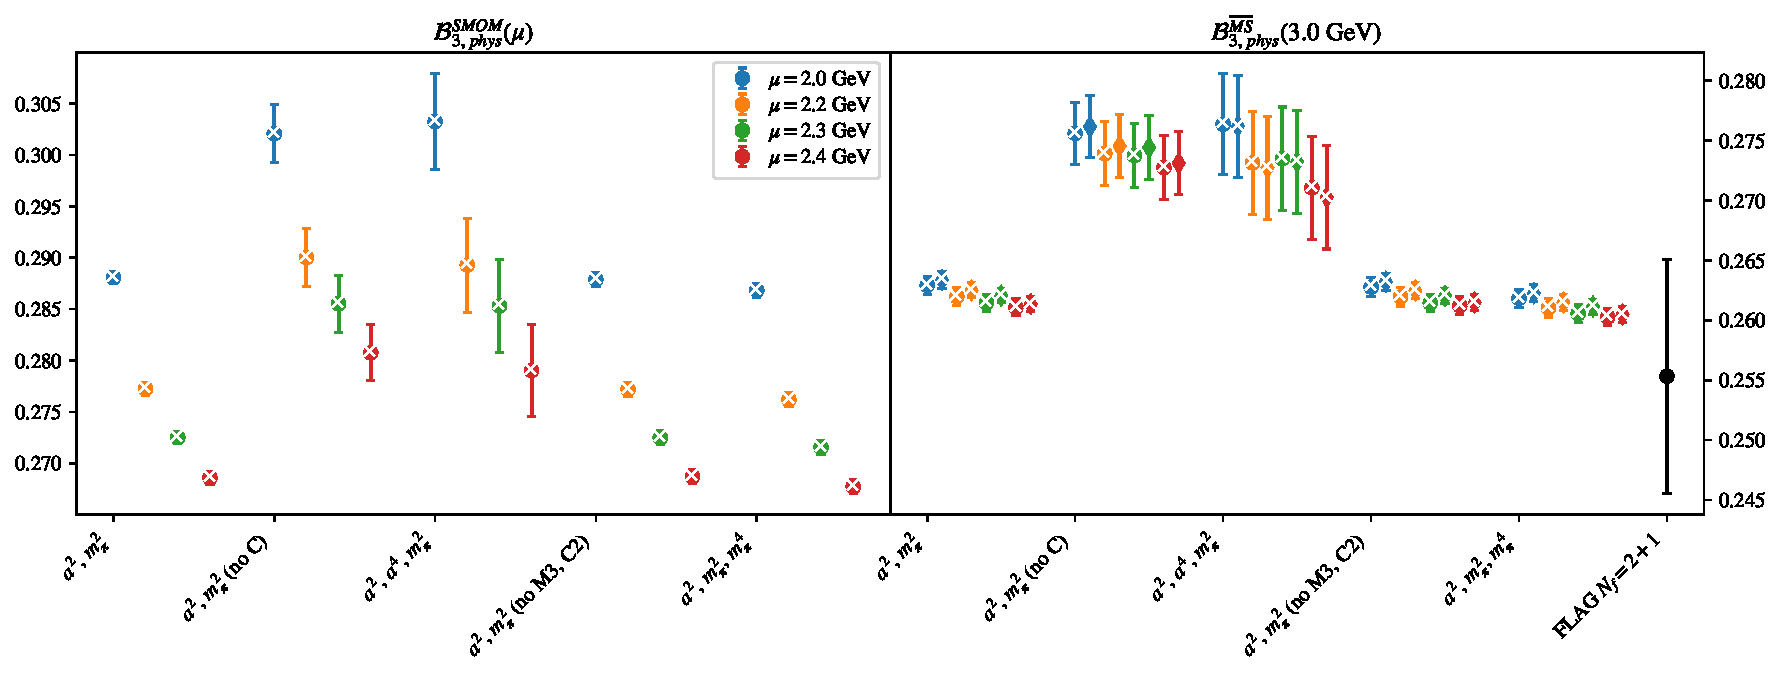
\includegraphics[page=1, width=1.1\textwidth]{SSmPP/SUSY/fit_summary_bag.pdf}
\caption{$\mathcal{B}_{3}$\\(left) $\mathcal{B}_{phys}$ in RI/SMOM scheme from fit variations (fits with $p$-value $<0.05$ marked with ``$\times$"). \\(right) $\mathcal{B}_{phys}$ in $\overline{MS}$ computed using $\mathcal{B}^{\overline{MS}} = R^{\overline{MS}\leftarrow SMOM}(3.0)\sigma_{npt}(3.0,\mu) \mathcal{B}^{SMOM}(\mu)$.}
\end{figure}
\clearpage
\begin{figure}
\centering
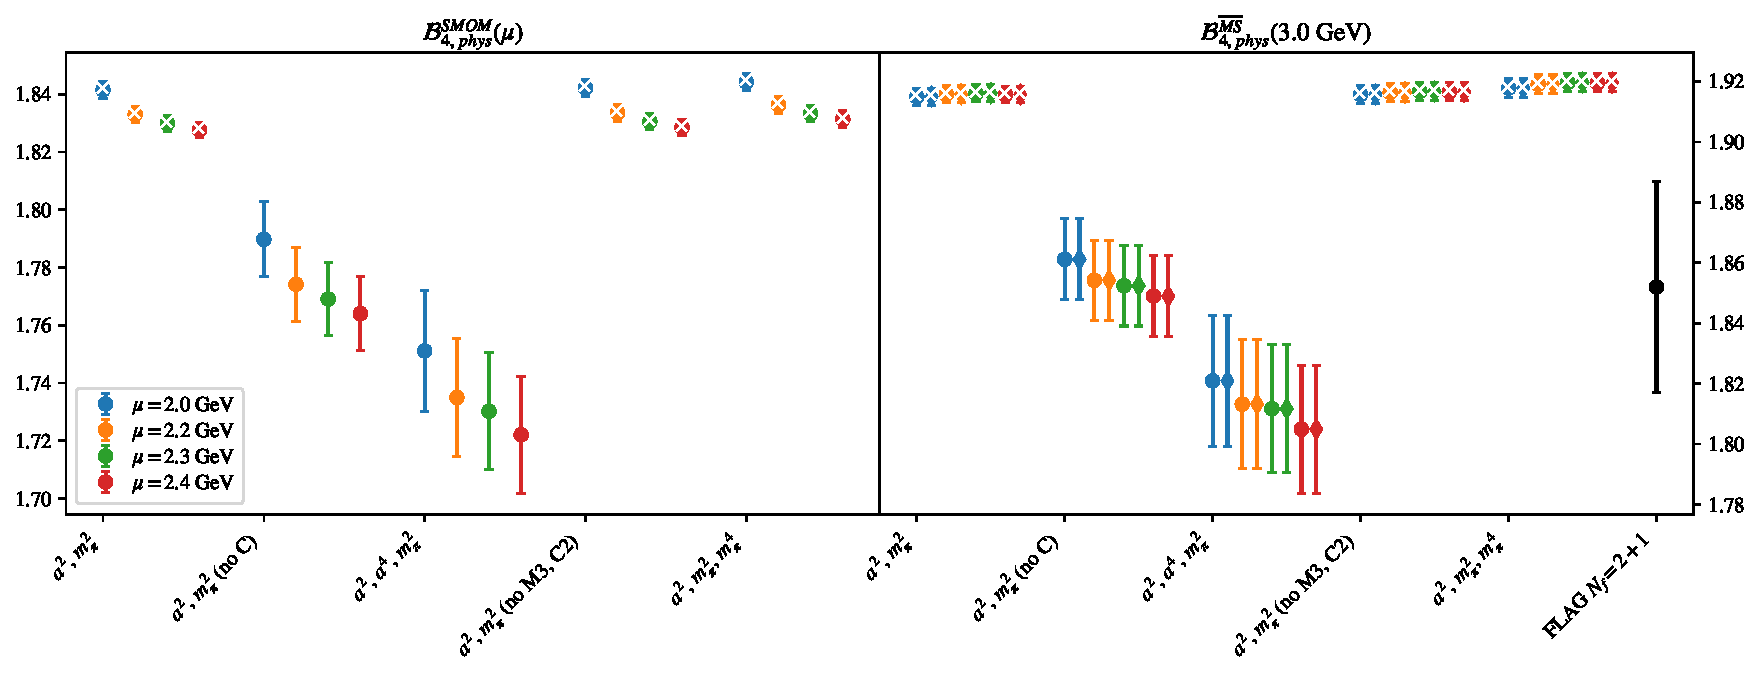
\includegraphics[page=1, width=1.1\textwidth]{SSpPP/SUSY/fit_summary_bag.pdf}
\caption{$\mathcal{B}_{4}$\\(left) $\mathcal{B}_{phys}$ in RI/SMOM scheme from fit variations (fits with $p$-value $<0.05$ marked with ``$\times$"). \\(right) $\mathcal{B}_{phys}$ in $\overline{MS}$ computed using $\mathcal{B}^{\overline{MS}} = R^{\overline{MS}\leftarrow SMOM}(3.0)\sigma_{npt}(3.0,\mu) \mathcal{B}^{SMOM}(\mu)$.}
\end{figure}
\clearpage
\begin{figure}
\centering
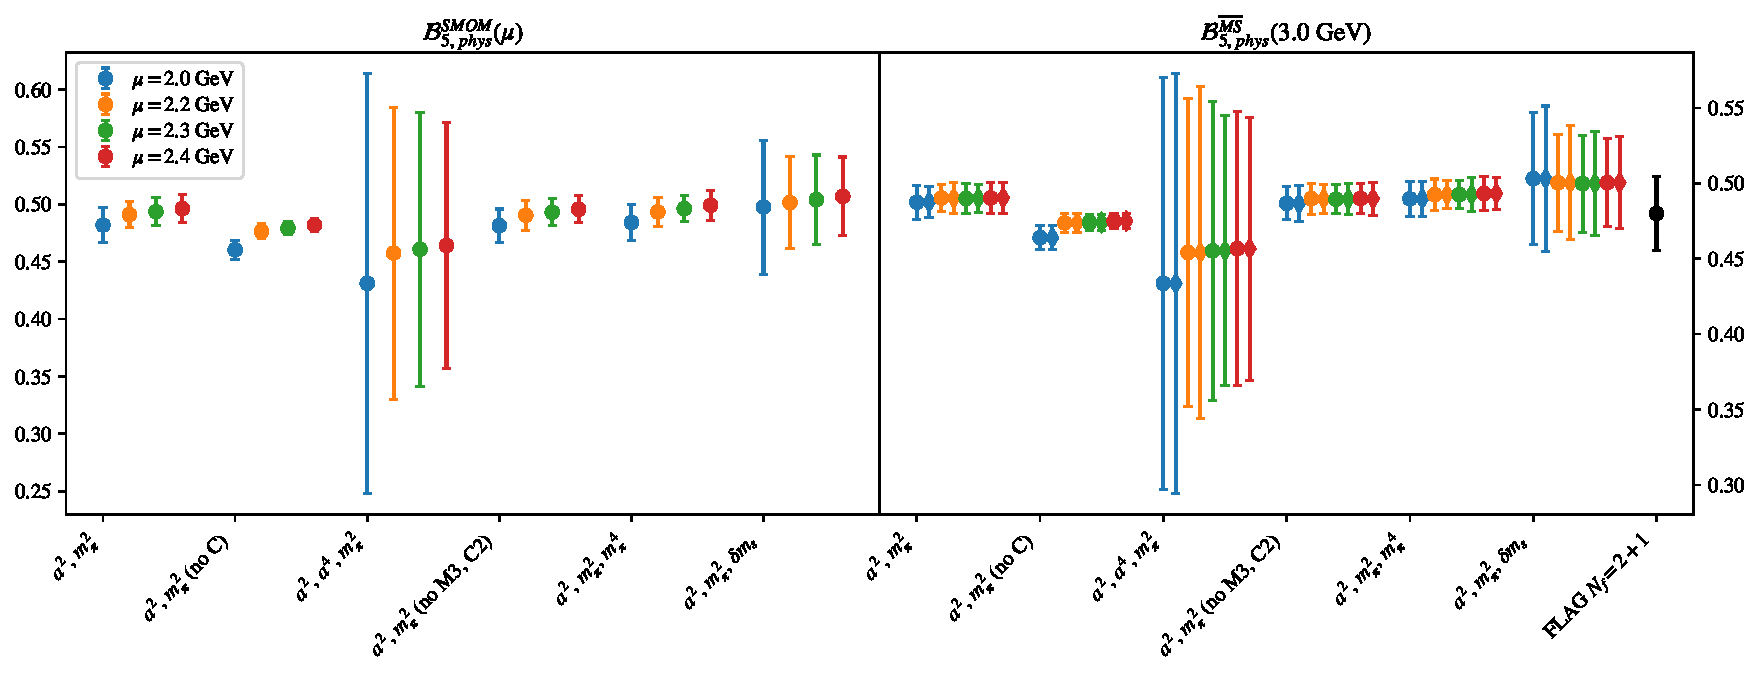
\includegraphics[page=1, width=1.1\textwidth]{TT/SUSY/fit_summary_bag.pdf}
\caption{$\mathcal{B}_{5}$\\(left) $\mathcal{B}_{phys}$ in RI/SMOM scheme from fit variations (fits with $p$-value $<0.05$ marked with ``$\times$"). \\(right) $\mathcal{B}_{phys}$ in $\overline{MS}$ computed using $\mathcal{B}^{\overline{MS}} = R^{\overline{MS}\leftarrow SMOM}(3.0)\sigma_{npt}(3.0,\mu) \mathcal{B}^{SMOM}(\mu)$.}
\end{figure}
\clearpage
\section{$\mathcal{B}_1$}
\begin{table}[h!]
\begin{center}
\begin{tabular}{|c|c|c|c|c|c|c|}
\hline
$\mu$ (GeV) & $a^2$, $m_\pi^2$& $a^2$, $m_\pi^2$ (no C)& $a^2$, $m_\pi^2$, $a^4$& $a^2$, $m_\pi^2$ (no M3, C2)& $a^2$, $m_\pi^2$, $m_\pi^4$& $a^2$, $m_\pi^2$, $\delta m_s$\\
\hline
2.0& \hyperlink{VVpAA/SUSY/bag_a2m2_20.pdf.1}{\textbf{1.4023(28)}: 2.369 (0.037)} & \hyperlink{VVpAA/SUSY/bag_a2m2noC_20.pdf.1}{\textbf{1.417(12)}: 0.897 (0.408)} & \hyperlink{VVpAA/SUSY/bag_a2a4m2_20.pdf.1}{\textbf{1.419(21)}: 2.81 (0.024)} & \hyperlink{VVpAA/SUSY/bag_a2m2mcut_20.pdf.1}{\textbf{1.4081(32)}: 0.284 (0.837)} & \hyperlink{VVpAA/SUSY/bag_a2m2m4_20.pdf.1}{\textbf{1.4081(33)}: 1.051 (0.379)} & \hyperlink{VVpAA/SUSY/bag_a2m2delm_20.pdf.1}{\textbf{1.3999(33)}: 2.41 (0.047)}\\
2.2& \hyperlink{VVpAA/SUSY/bag_a2m2_22.pdf.1}{\textbf{1.3949(28)}: 2.686 (0.02)} & \hyperlink{VVpAA/SUSY/bag_a2m2noC_22.pdf.1}{\textbf{1.412(12)}: 1.029 (0.357)} & \hyperlink{VVpAA/SUSY/bag_a2a4m2_22.pdf.1}{\textbf{1.415(21)}: 3.131 (0.014)} & \hyperlink{VVpAA/SUSY/bag_a2m2mcut_22.pdf.1}{\textbf{1.4010(32)}: 0.415 (0.742)} & \hyperlink{VVpAA/SUSY/bag_a2m2m4_22.pdf.1}{\textbf{1.4009(33)}: 1.272 (0.278)} & \hyperlink{VVpAA/SUSY/bag_a2m2delm_22.pdf.1}{\textbf{1.3922(33)}: 2.622 (0.033)}\\
2.3& \hyperlink{VVpAA/SUSY/bag_a2m2_23.pdf.1}{\textbf{1.3913(27)}: 2.92 (0.012)} & \hyperlink{VVpAA/SUSY/bag_a2m2noC_23.pdf.1}{\textbf{1.409(12)}: 1.106 (0.331)} & \hyperlink{VVpAA/SUSY/bag_a2a4m2_23.pdf.1}{\textbf{1.413(21)}: 3.381 (0.009)} & \hyperlink{VVpAA/SUSY/bag_a2m2mcut_23.pdf.1}{\textbf{1.3977(32)}: 0.499 (0.683)} & \hyperlink{VVpAA/SUSY/bag_a2m2m4_23.pdf.1}{\textbf{1.3975(33)}: 1.443 (0.217)} & \hyperlink{VVpAA/SUSY/bag_a2m2delm_23.pdf.1}{\textbf{1.3885(32)}: 2.792 (0.025)}\\
2.4& \hyperlink{VVpAA/SUSY/bag_a2m2_24.pdf.1}{\textbf{1.3884(27)}: 3.03 (0.01)} & \hyperlink{VVpAA/SUSY/bag_a2m2noC_24.pdf.1}{\textbf{1.407(12)}: 1.156 (0.315)} & \hyperlink{VVpAA/SUSY/bag_a2a4m2_24.pdf.1}{\textbf{1.411(20)}: 3.505 (0.007)} & \hyperlink{VVpAA/SUSY/bag_a2m2mcut_24.pdf.1}{\textbf{1.3949(32)}: 0.528 (0.663)} & \hyperlink{VVpAA/SUSY/bag_a2m2m4_24.pdf.1}{\textbf{1.3946(33)}: 1.509 (0.196)} & \hyperlink{VVpAA/SUSY/bag_a2m2delm_24.pdf.1}{\textbf{1.3854(32)}: 2.879 (0.021)}\\
\hline
\end{tabular}
\caption{Physical point value from chiral and continuum extrapolation at renormalisation scale $\mu$. Entries are \textbf{value(error)}: $\chi^2/\text{DOF}$ ($p$-value).}
\end{center}
\end{table}
\begin{table}[h!]
\begin{center}
\begin{tabular}{|c c|c|c|c|c|c|c|}
\hline
$\mu$ (GeV) &  & $a^2$, $m_\pi^2$& $a^2$, $m_\pi^2$ (no C)& $a^2$, $m_\pi^2$, $a^4$& $a^2$, $m_\pi^2$ (no M3, C2)& $a^2$, $m_\pi^2$, $m_\pi^4$& $a^2$, $m_\pi^2$, $\delta m_s$\\
\hline
\multirow{3}{0.5in}{2.0} & $\alpha$ & 0.138(10)& 0.065(76)& -0.01(19)& 0.119(11)& 0.120(11)& 0.146(11)\\
 & $\beta$ & 0.00400(21)& 0.00326(42)& 0.00408(23)& 0.00286(42)& 0.0005(12)& 0.00415(23)\\
 & $\gamma$ &  &  & 0.31(40)&  & 0.00031(11)& -0.0048(33)\\
\hline
\multirow{3}{0.5in}{2.2} & $\alpha$ & 0.143(10)& 0.056(75)& -0.04(19)& 0.123(11)& 0.124(11)& 0.152(11)\\
 & $\beta$ & 0.00391(20)& 0.00314(41)& 0.00401(23)& 0.00272(41)& 0.0003(12)& 0.00408(23)\\
 & $\gamma$ &  &  & 0.38(40)&  & 0.00032(11)& -0.0055(33)\\
\hline
\multirow{3}{0.5in}{2.3} & $\alpha$ & 0.146(10)& 0.052(74)& -0.06(19)& 0.125(11)& 0.126(11)& 0.155(11)\\
 & $\beta$ & 0.00388(20)& 0.00308(41)& 0.00399(23)& 0.00266(41)& 0.0001(12)& 0.00407(22)\\
 & $\gamma$ &  &  & 0.41(39)&  & 0.00033(10)& -0.0059(33)\\
\hline
\multirow{3}{0.5in}{2.4} & $\alpha$ & 0.1468(99)& 0.050(74)& -0.06(19)& 0.125(11)& 0.127(11)& 0.156(11)\\
 & $\beta$ & 0.00386(20)& 0.00305(40)& 0.00397(22)& 0.00263(41)& 0.00009(126)& 0.00405(22)\\
 & $\gamma$ &  &  & 0.42(39)&  & 0.00033(10)& -0.0061(32)\\
\hline
\end{tabular}
\caption{Fit values of coefficients in $Q = Q_{phys} + \mathbf{\alpha} a^2 + \mathbf{\beta}\left(\frac{m_\pi^2}{f_\pi^2}-\frac{m_{\pi,PDG}^2}{f_\pi^2}\right) + \gamma(\ldots)$}
\end{center}
\end{table}
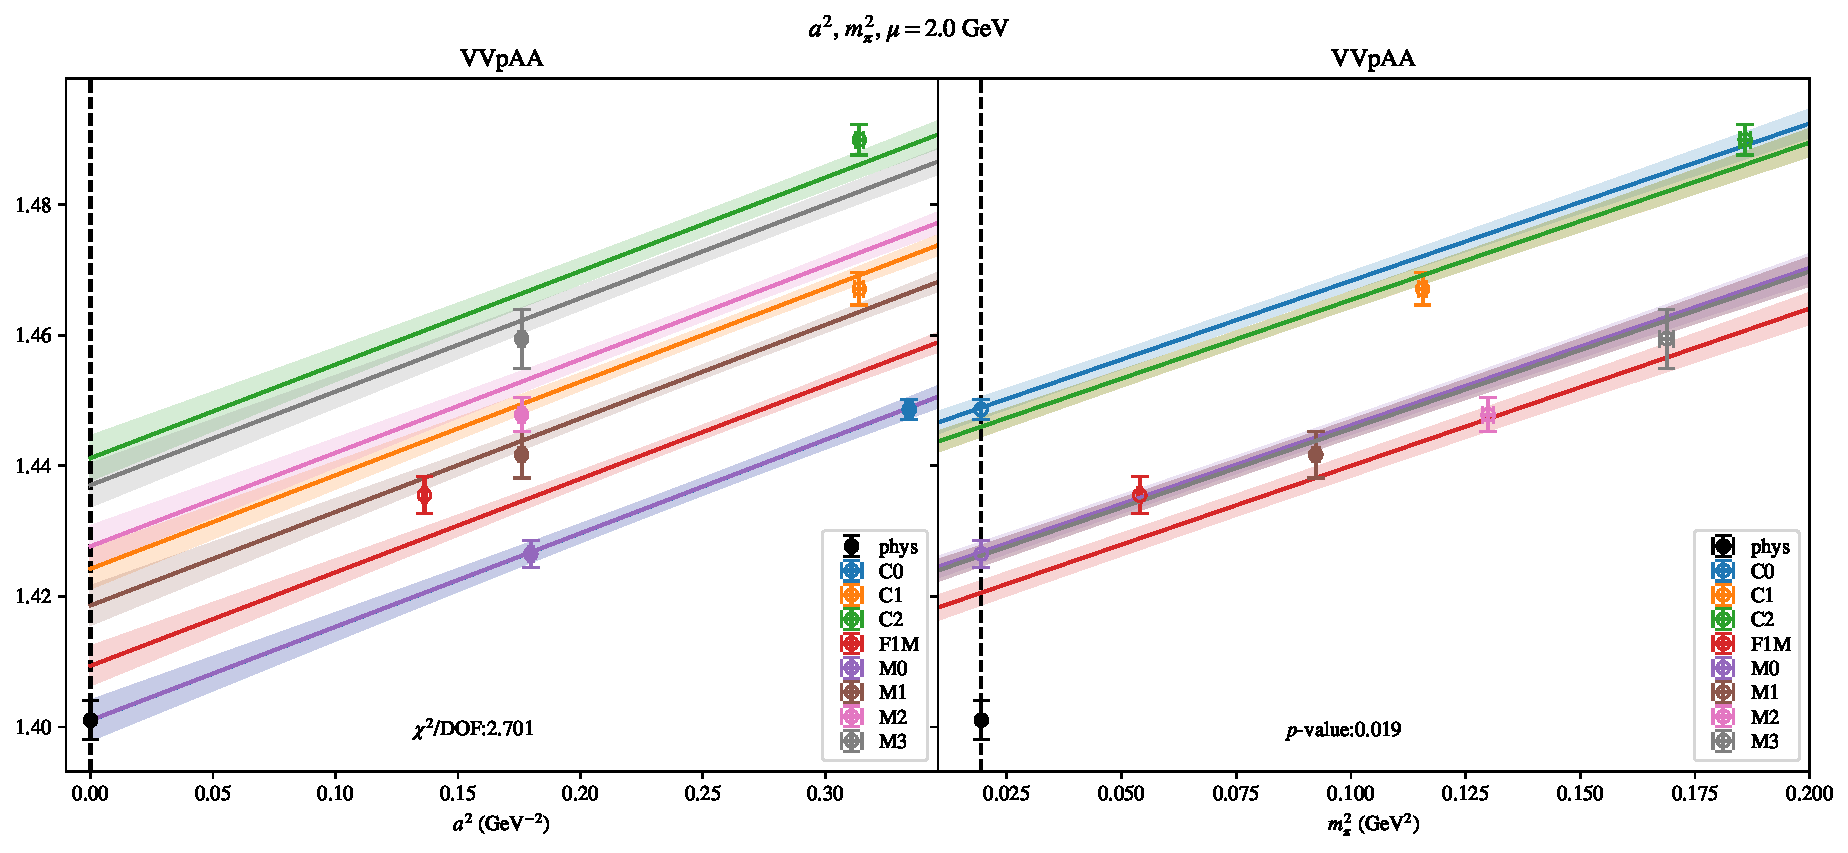
\includepdf[link, pages=-]{VVpAA/SUSY/bag_a2m2_20.pdf}
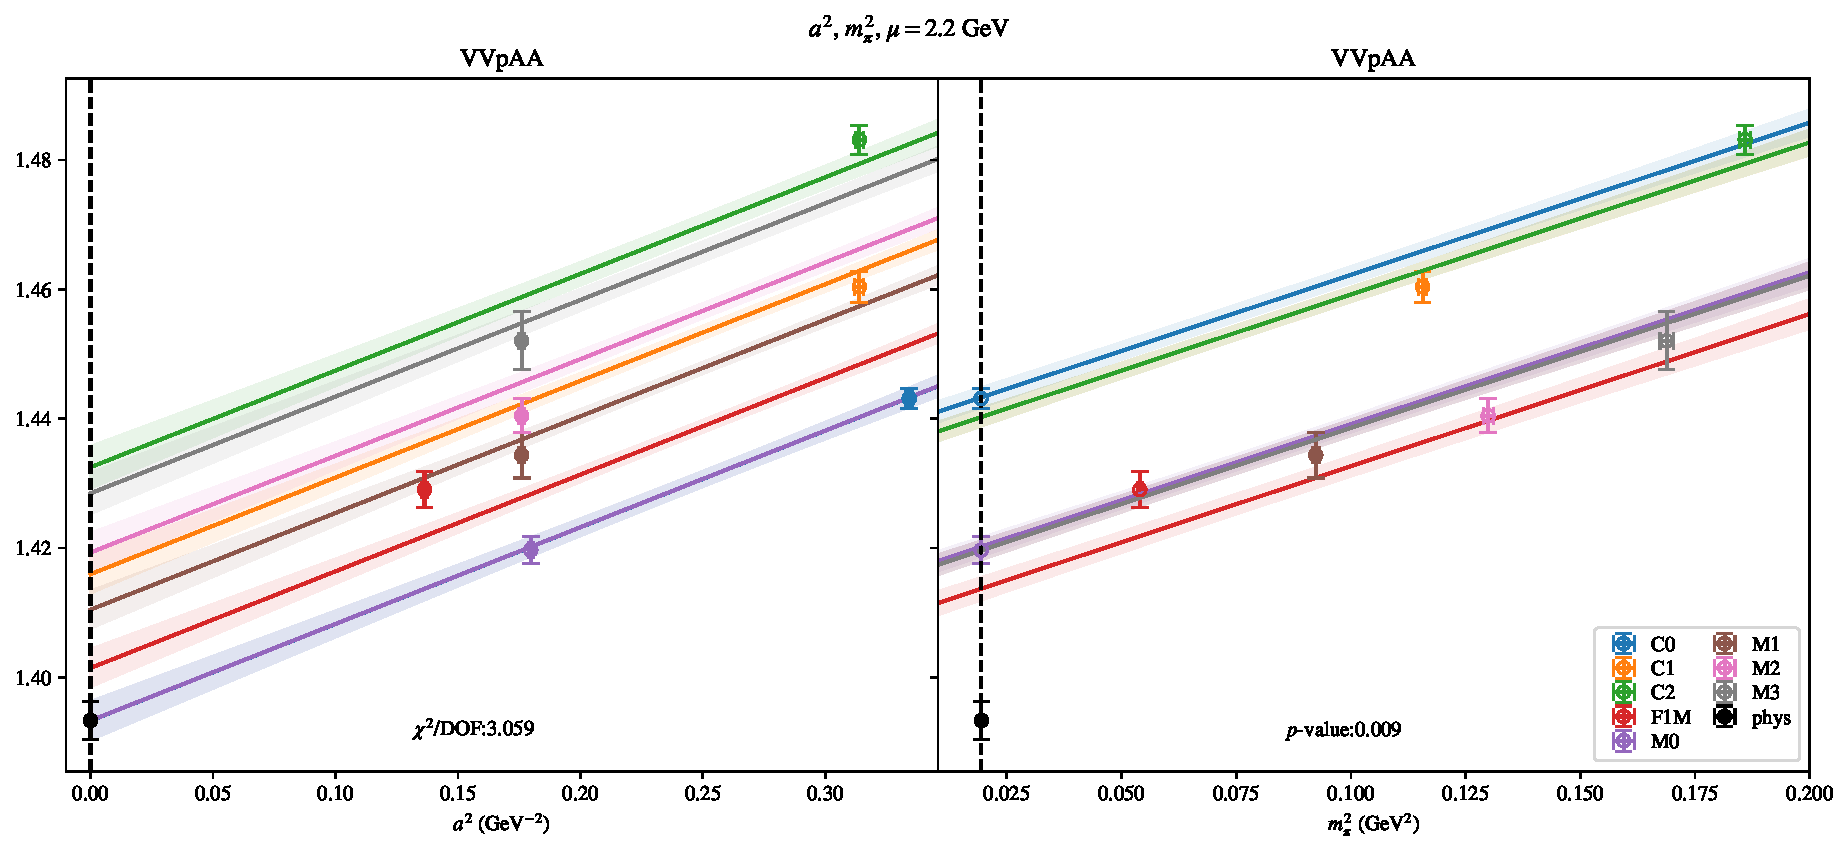
\includepdf[link, pages=-]{VVpAA/SUSY/bag_a2m2_22.pdf}
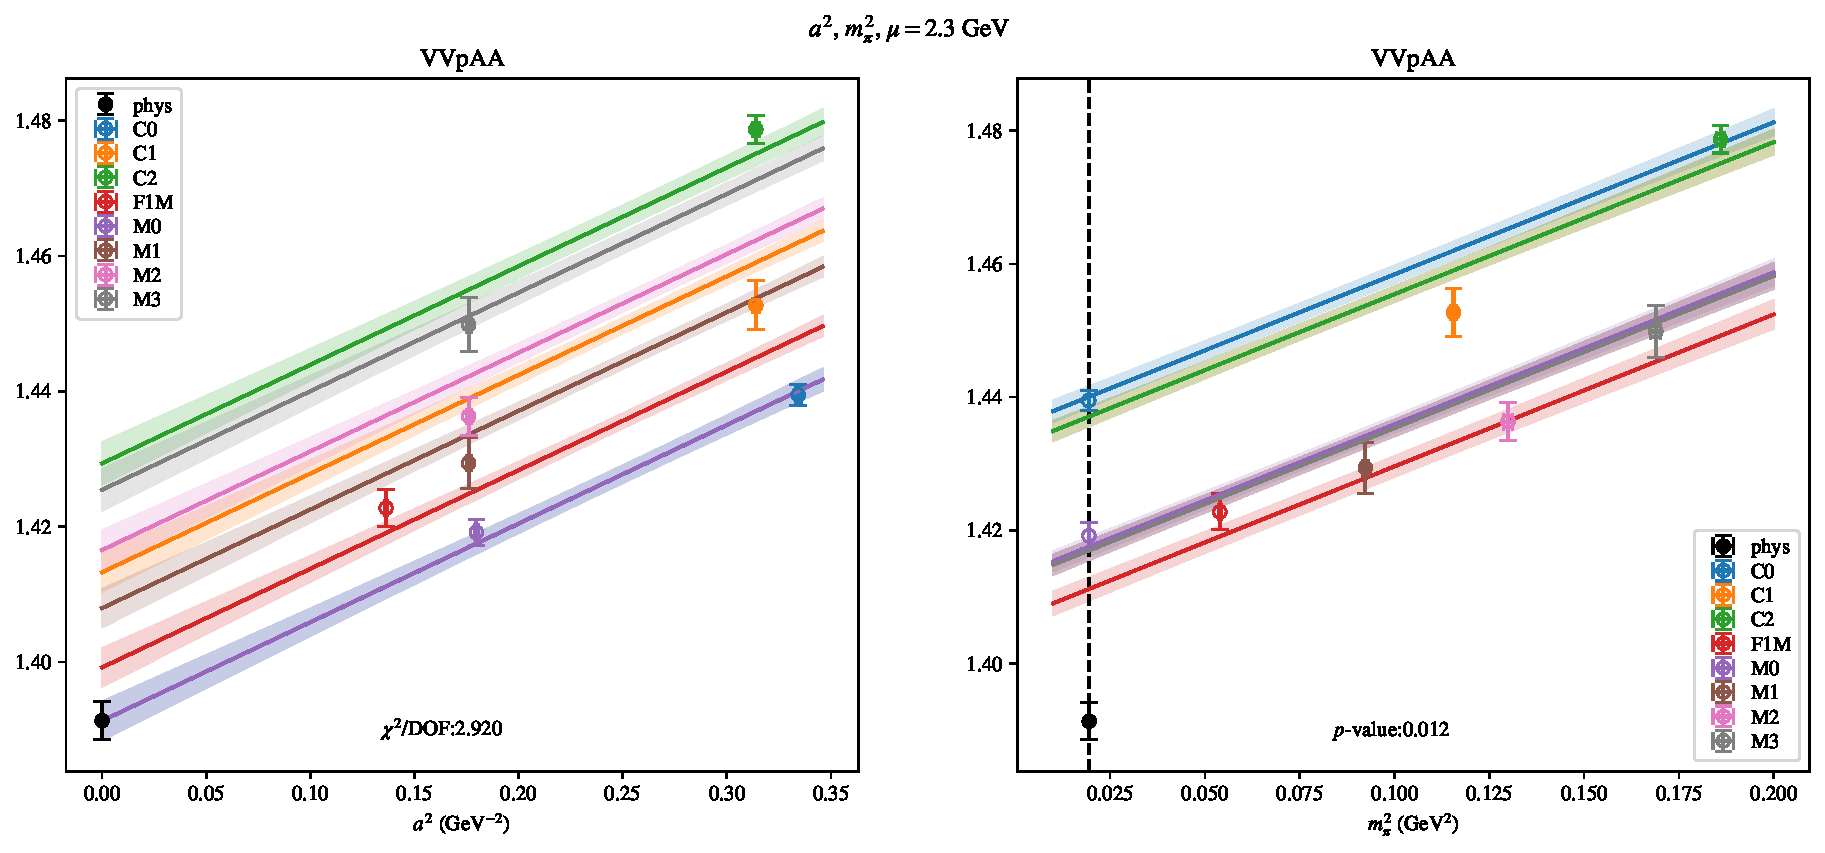
\includepdf[link, pages=-]{VVpAA/SUSY/bag_a2m2_23.pdf}
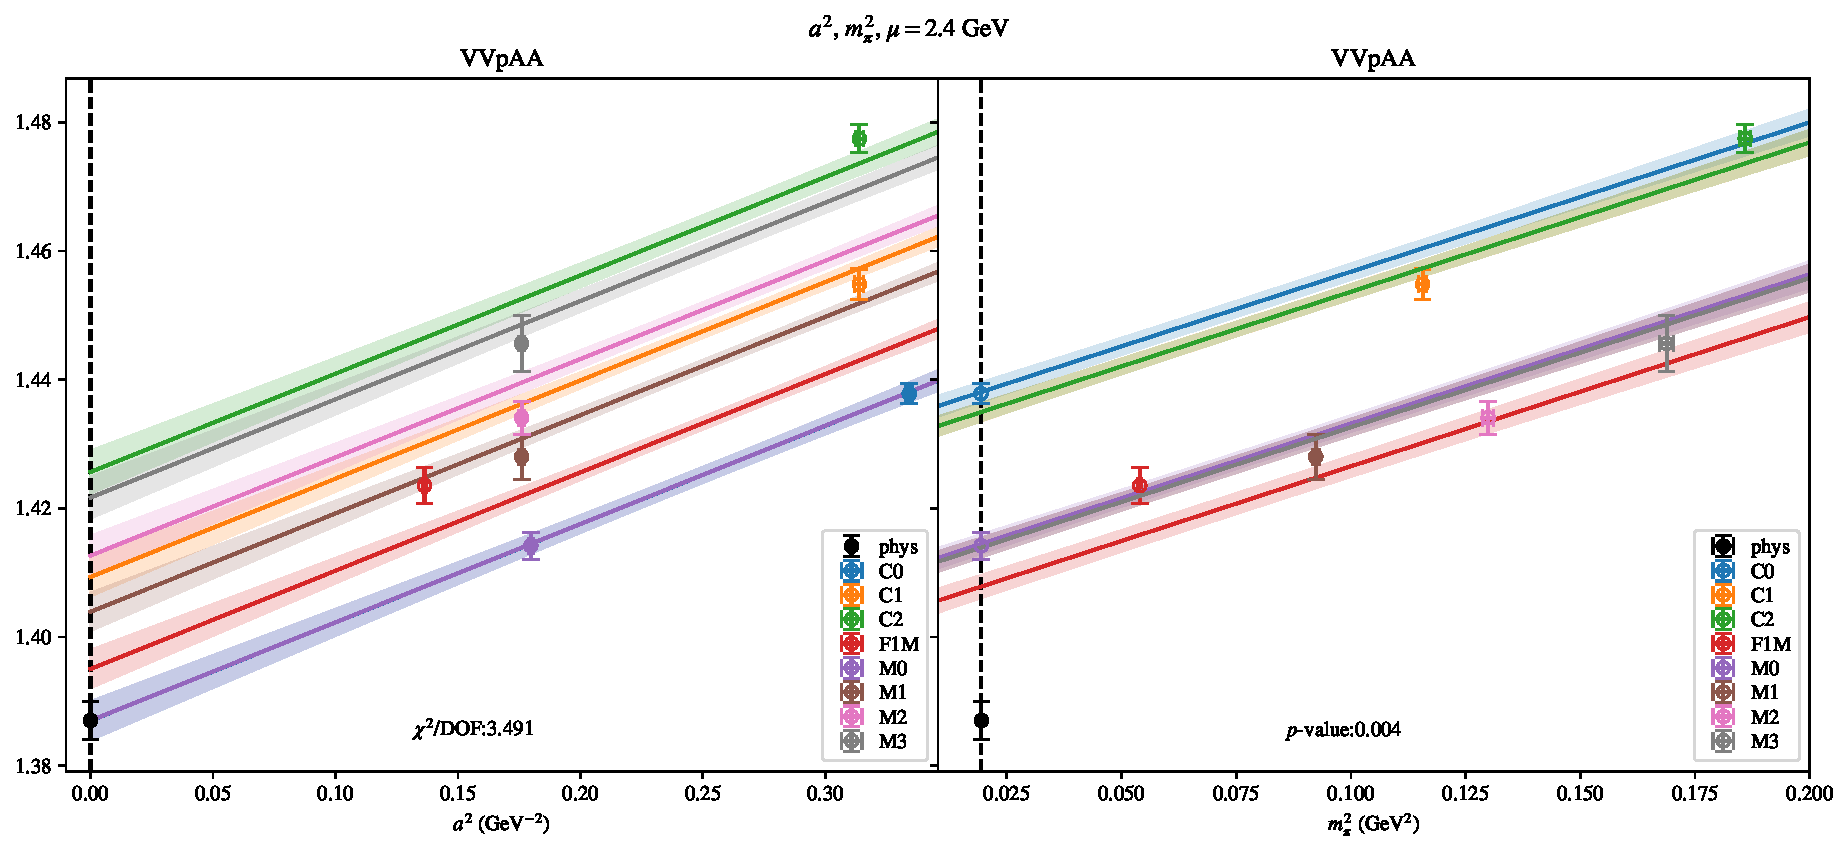
\includepdf[link, pages=-]{VVpAA/SUSY/bag_a2m2_24.pdf}
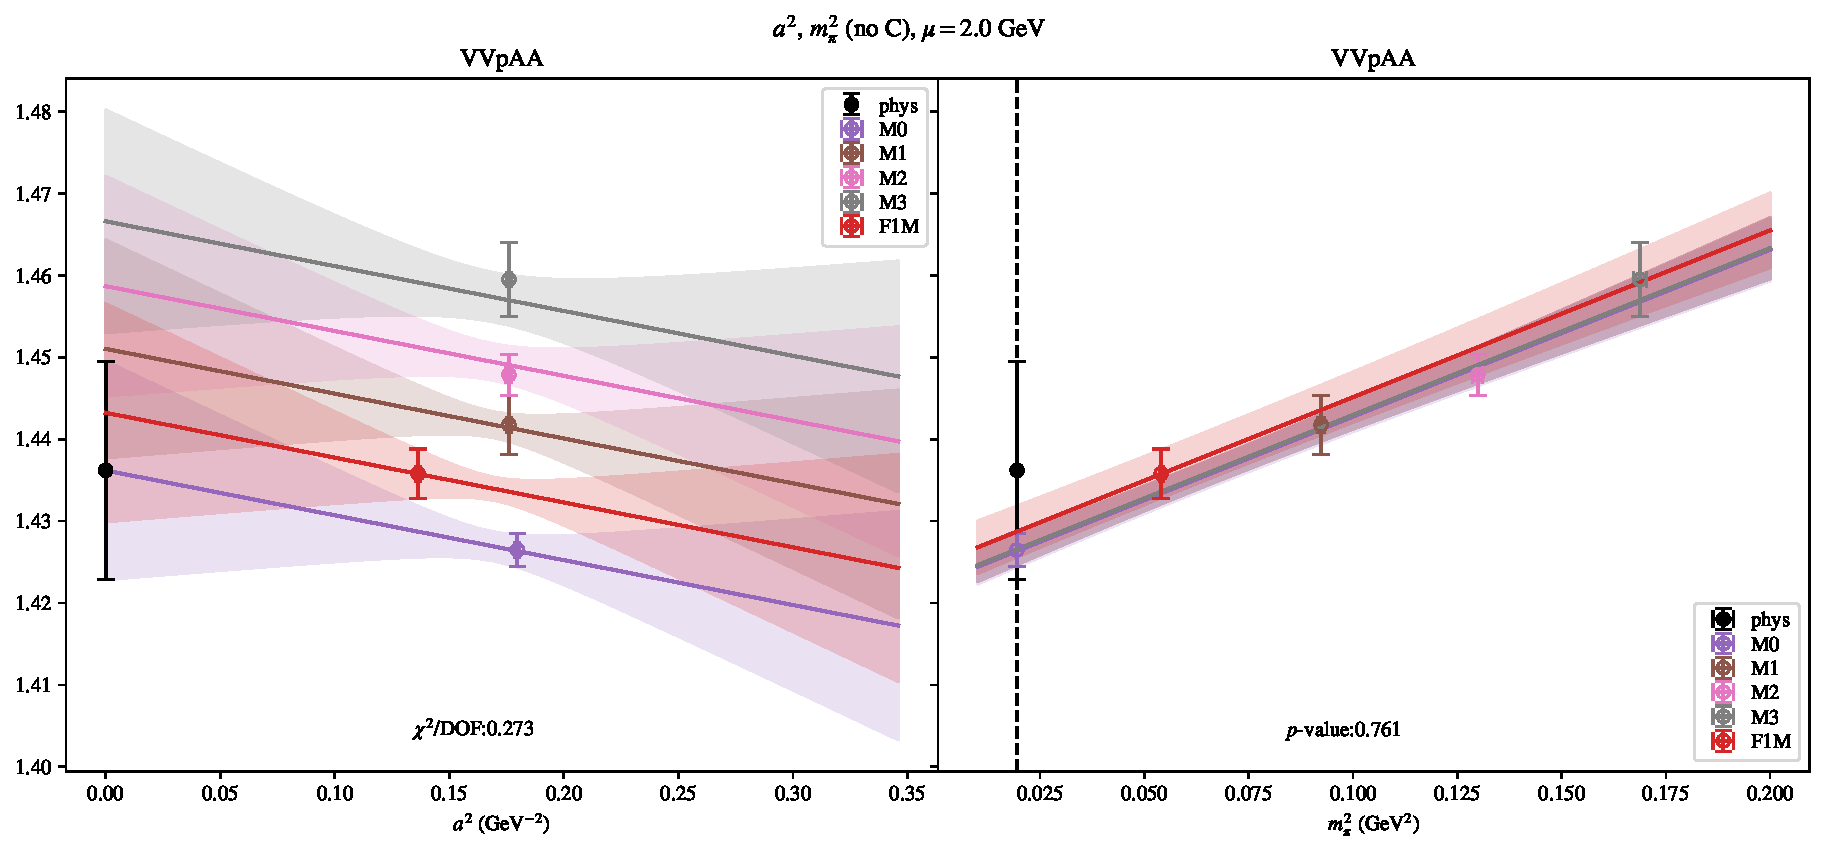
\includepdf[link, pages=-]{VVpAA/SUSY/bag_a2m2noC_20.pdf}
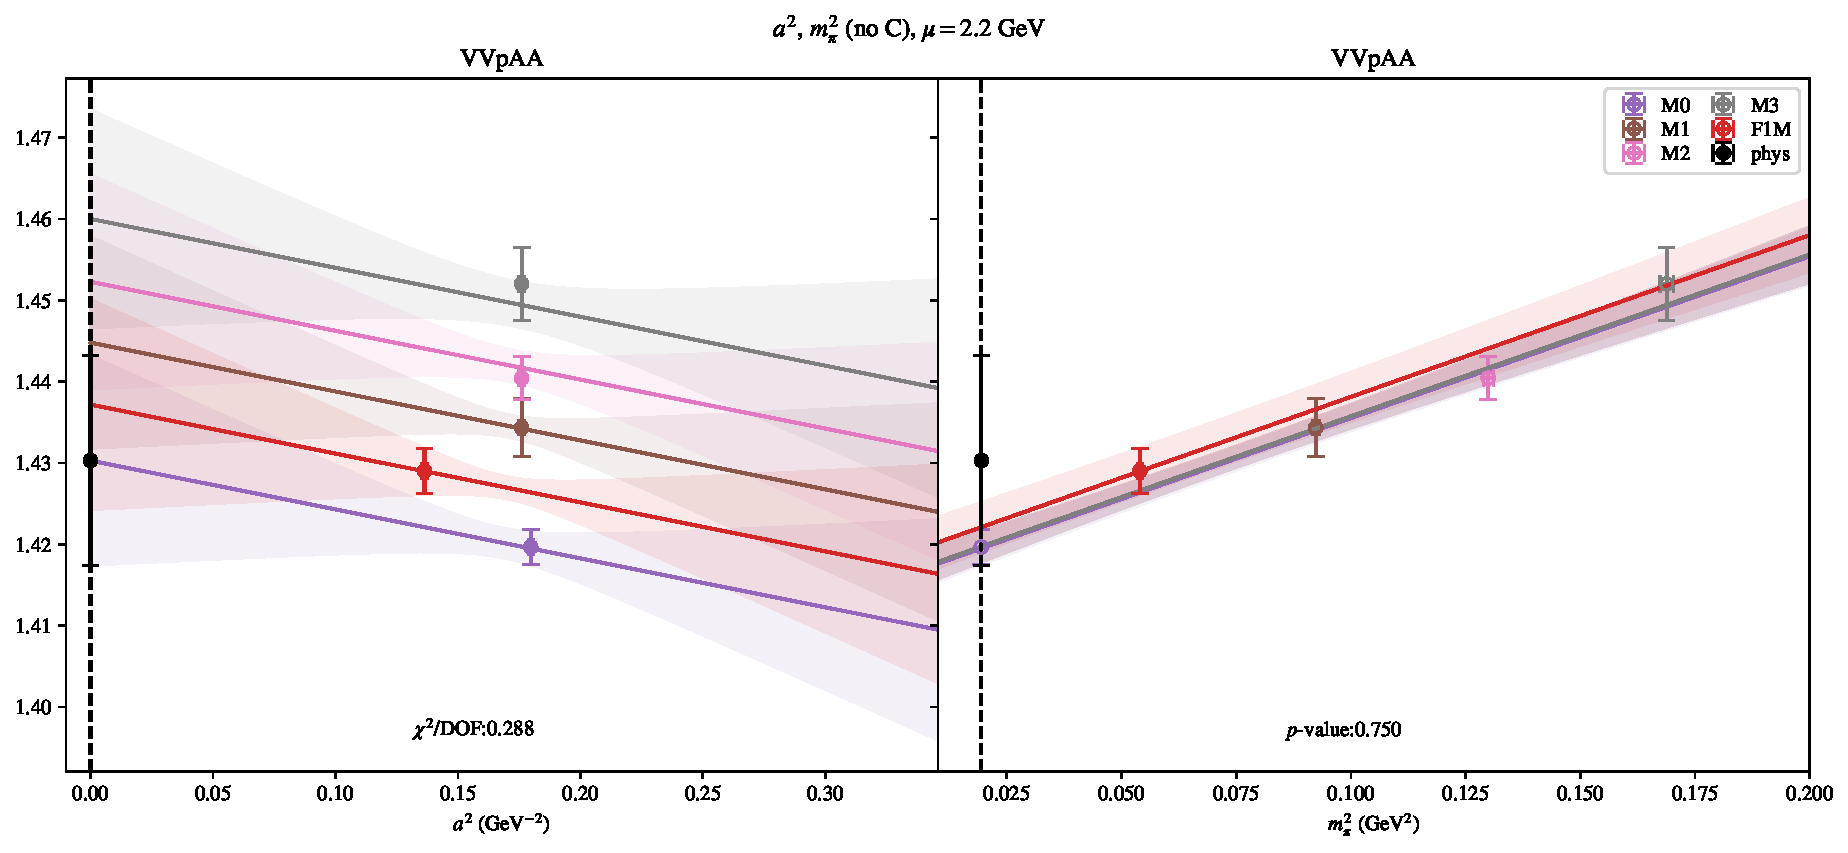
\includepdf[link, pages=-]{VVpAA/SUSY/bag_a2m2noC_22.pdf}
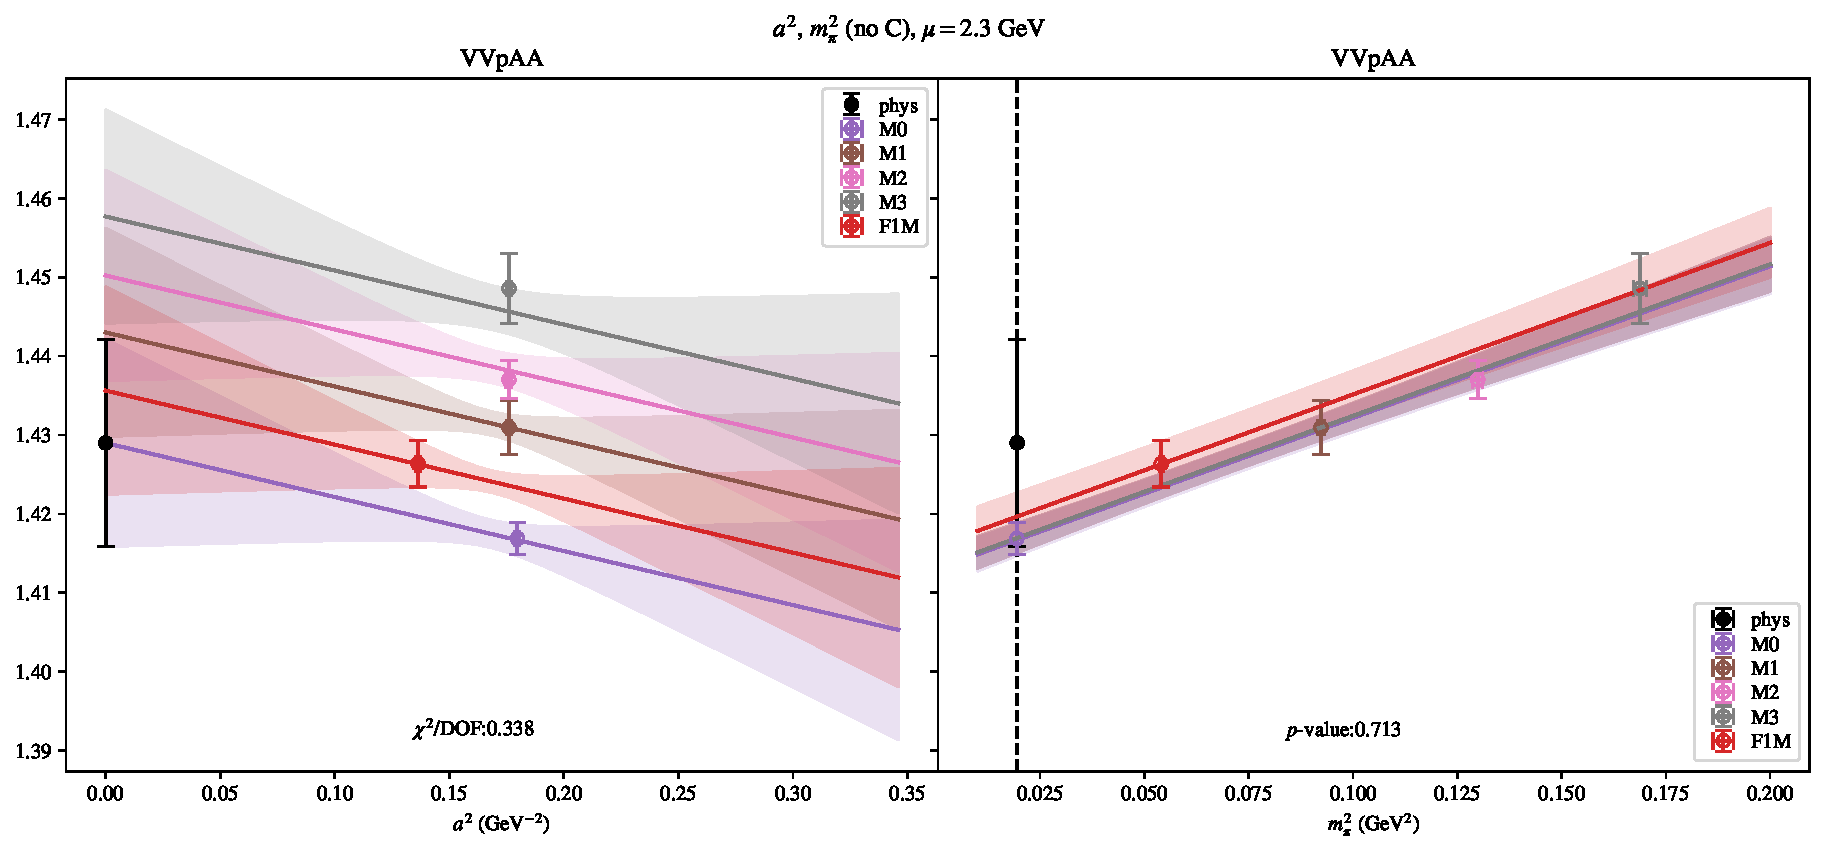
\includepdf[link, pages=-]{VVpAA/SUSY/bag_a2m2noC_23.pdf}
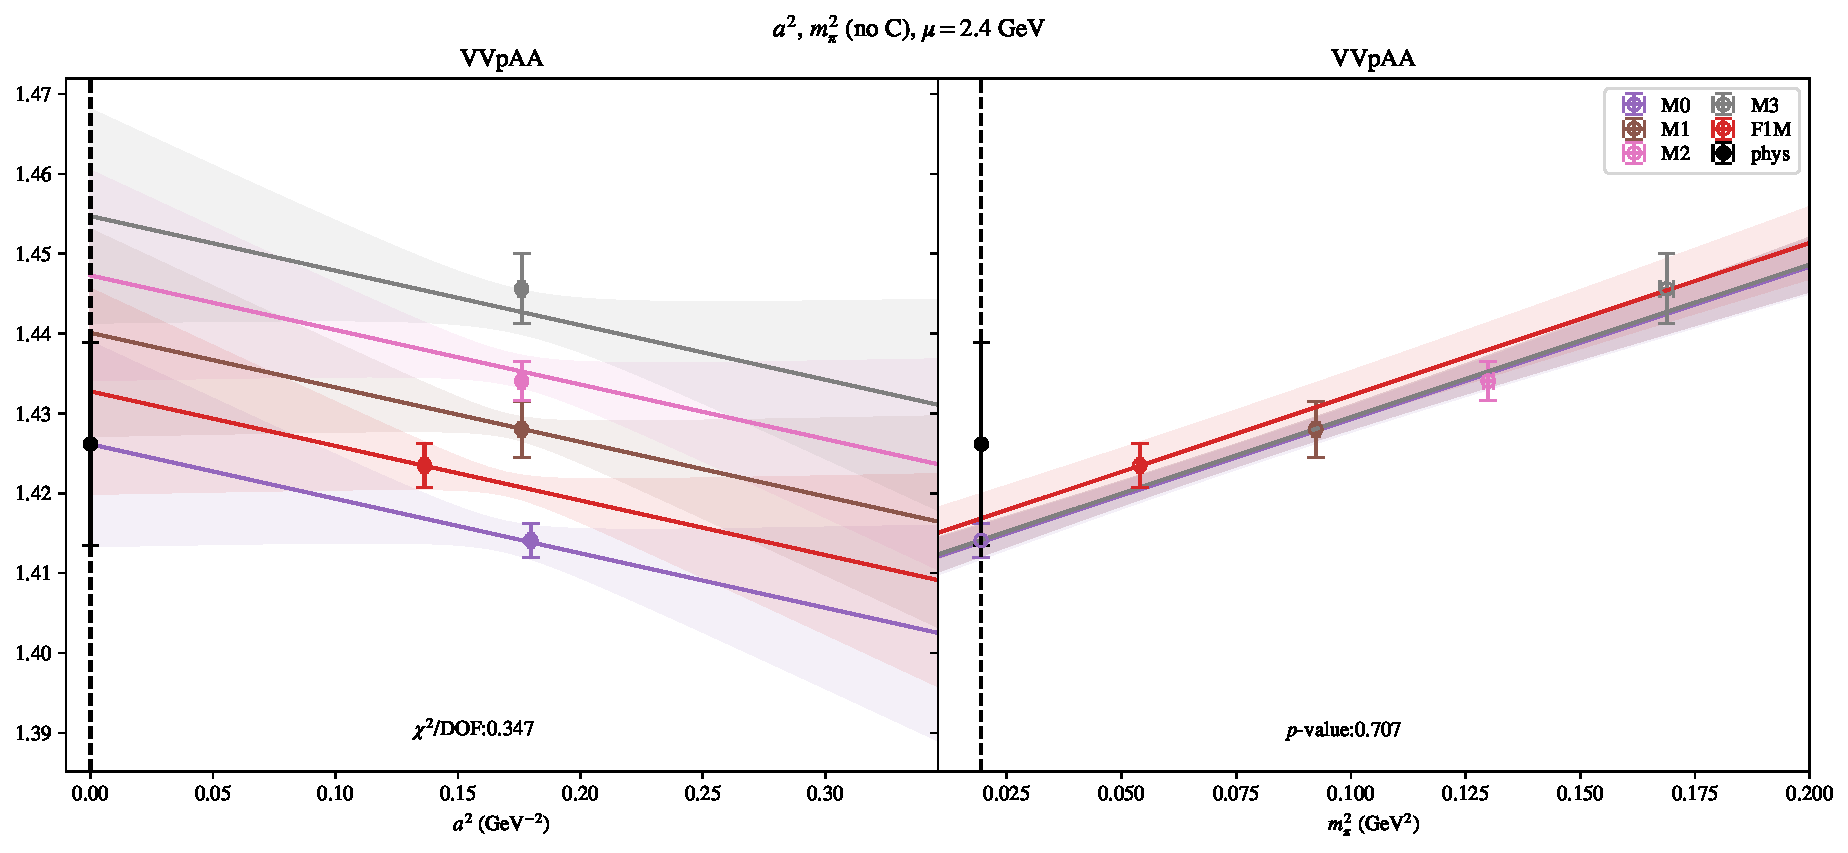
\includepdf[link, pages=-]{VVpAA/SUSY/bag_a2m2noC_24.pdf}
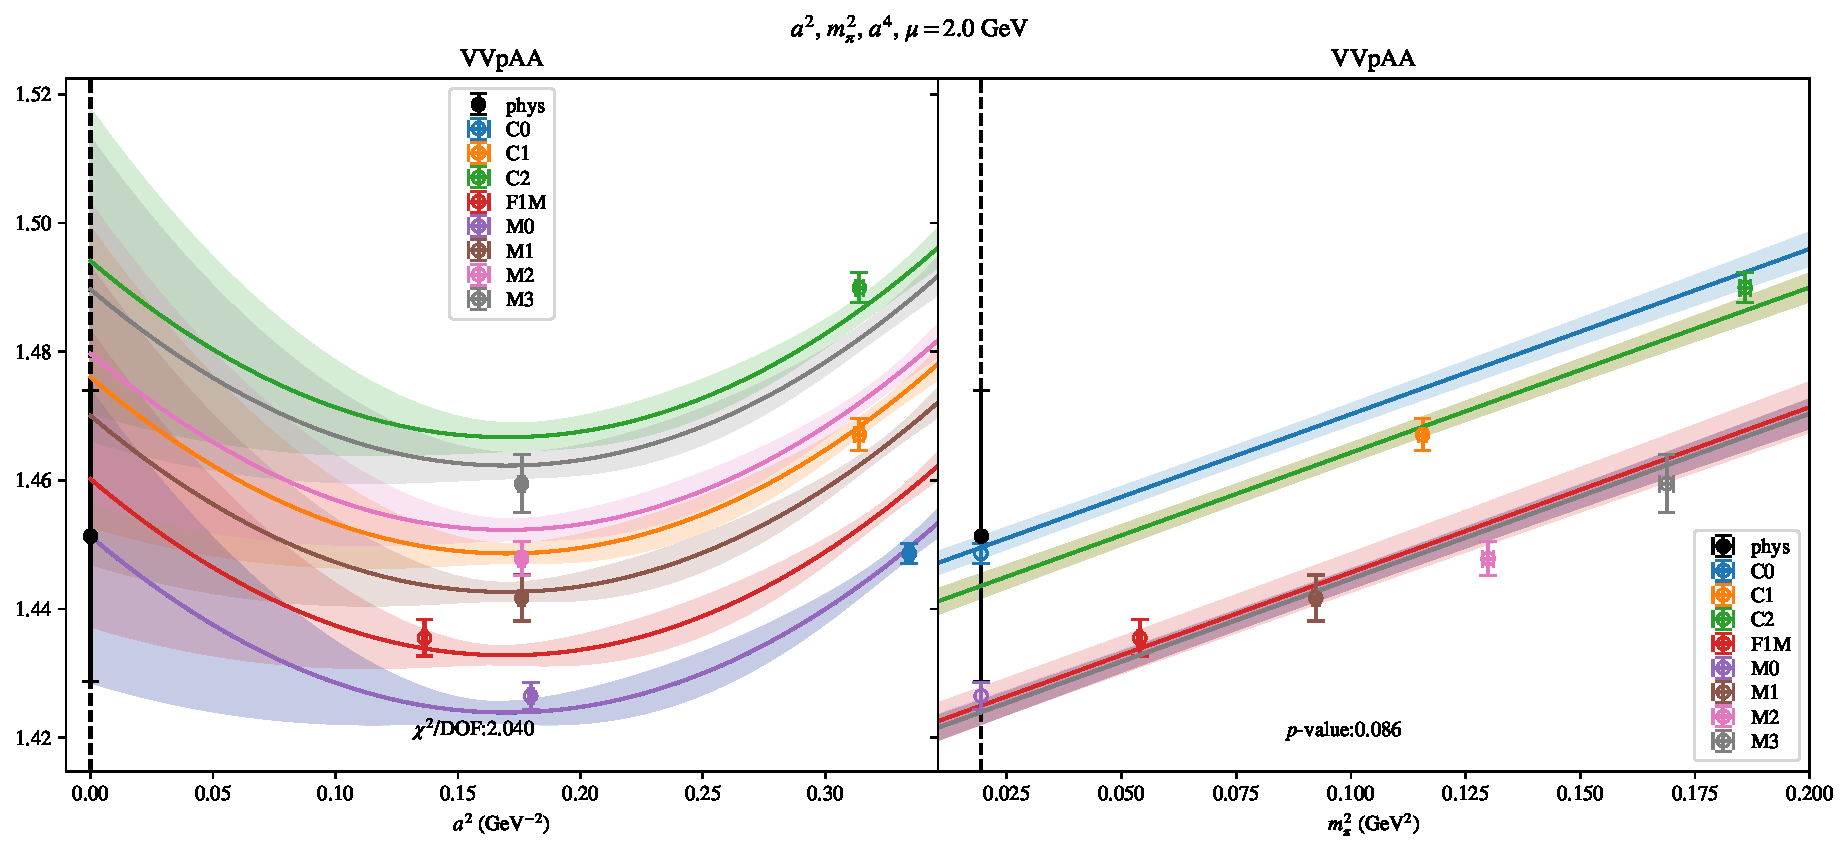
\includepdf[link, pages=-]{VVpAA/SUSY/bag_a2a4m2_20.pdf}
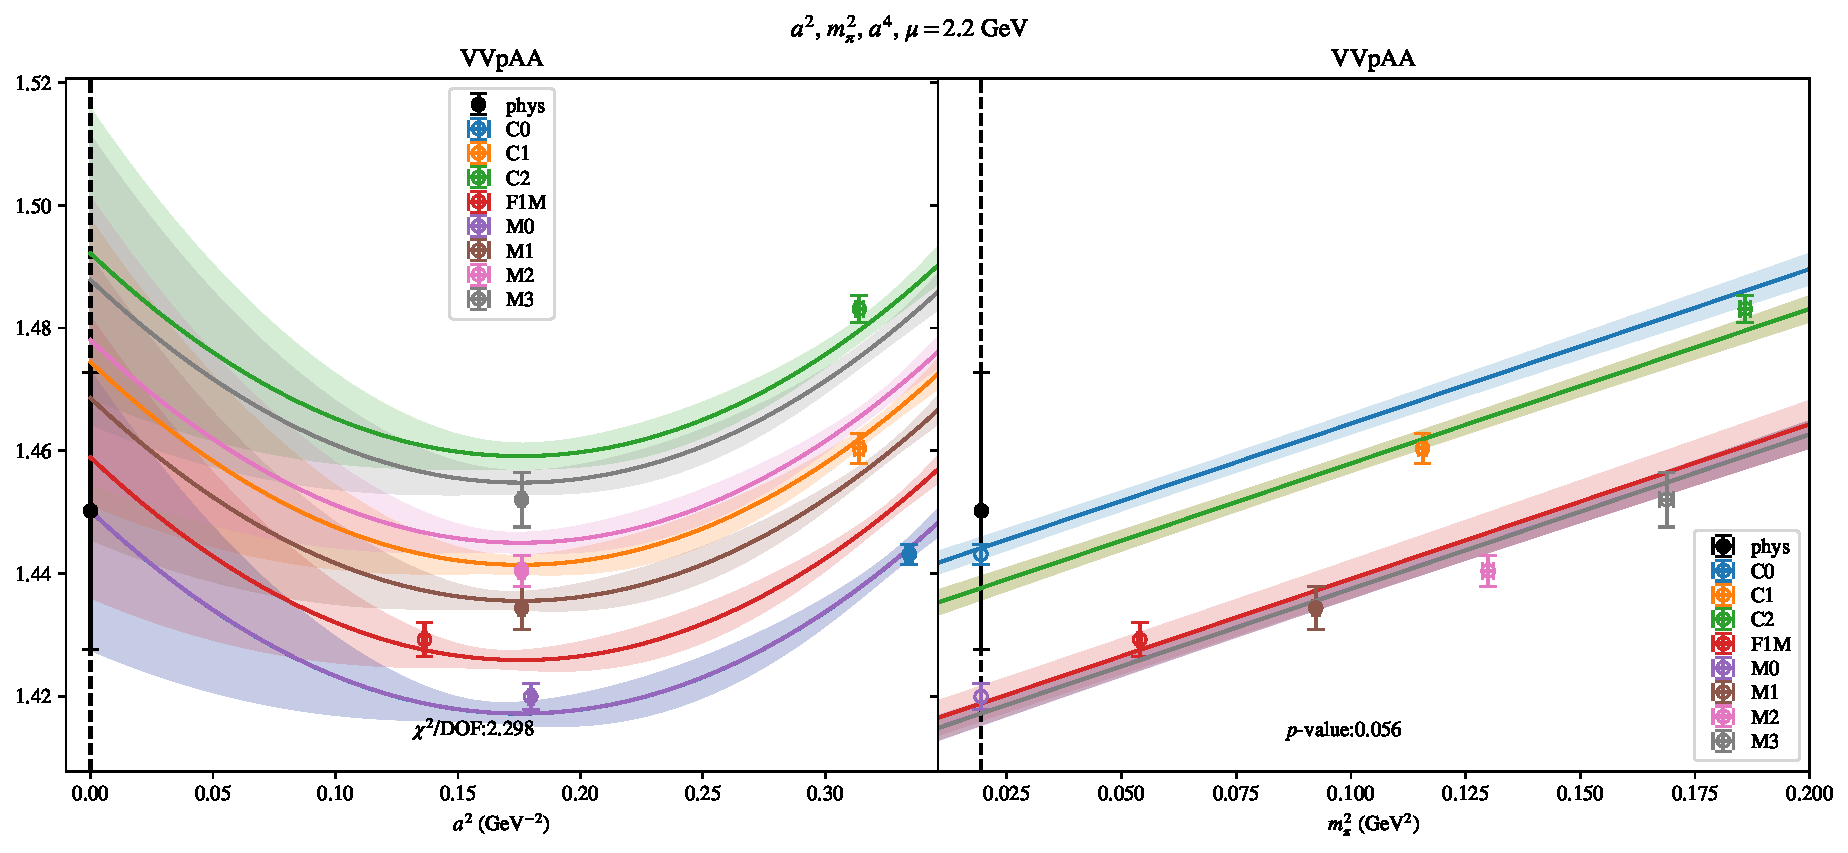
\includepdf[link, pages=-]{VVpAA/SUSY/bag_a2a4m2_22.pdf}
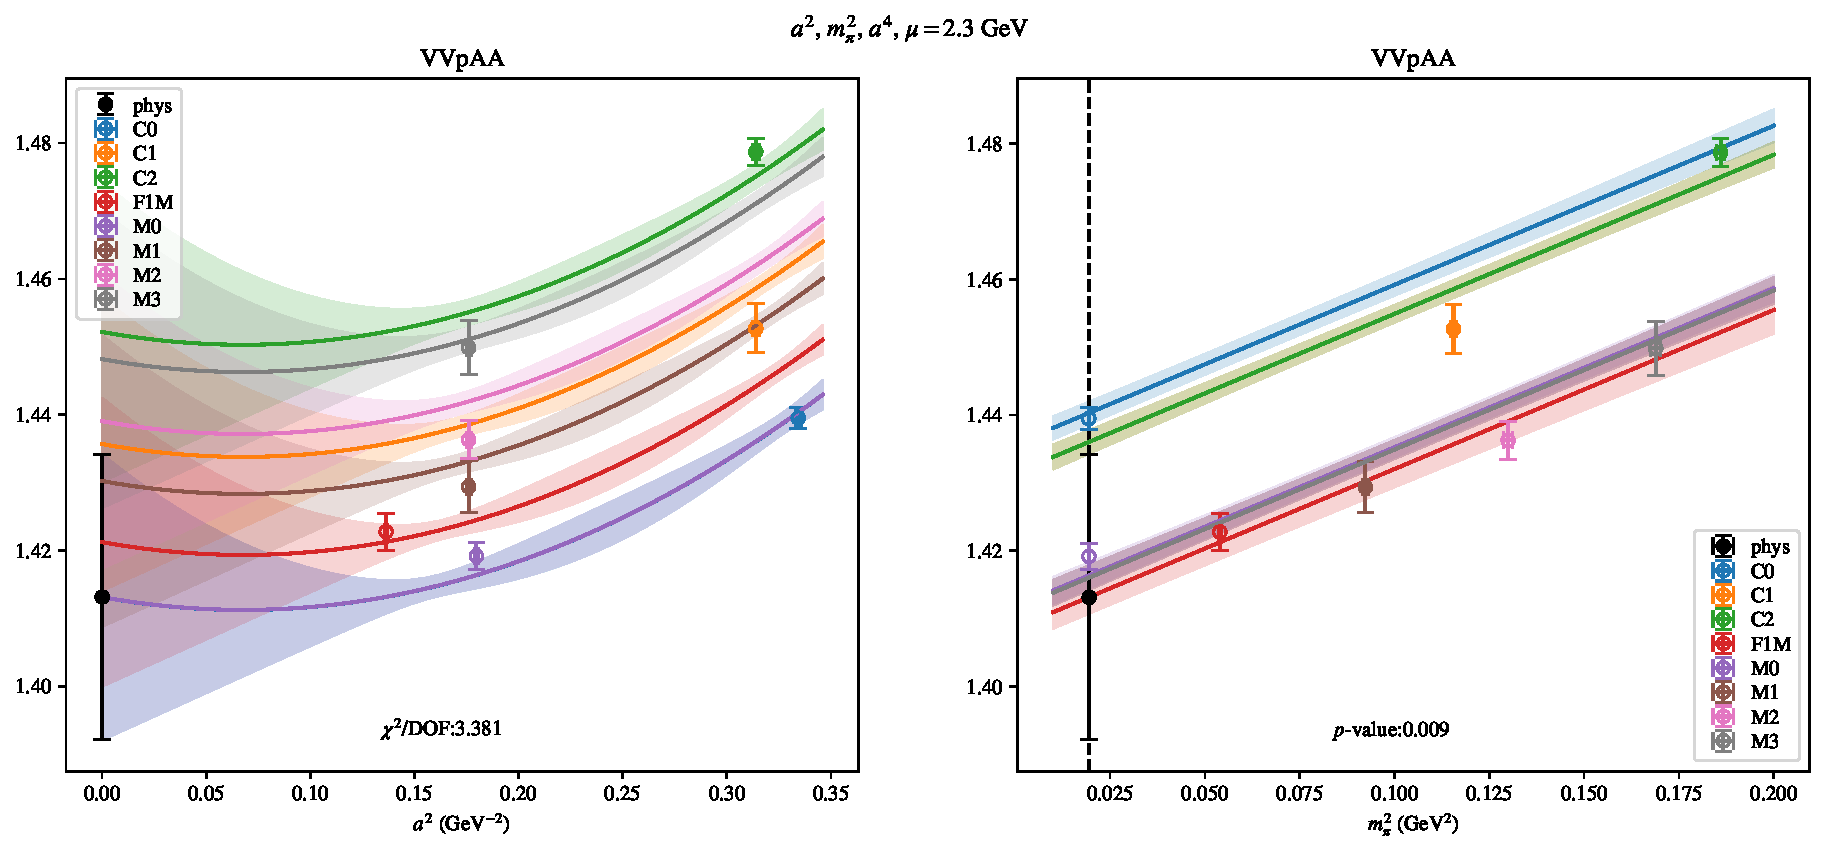
\includepdf[link, pages=-]{VVpAA/SUSY/bag_a2a4m2_23.pdf}
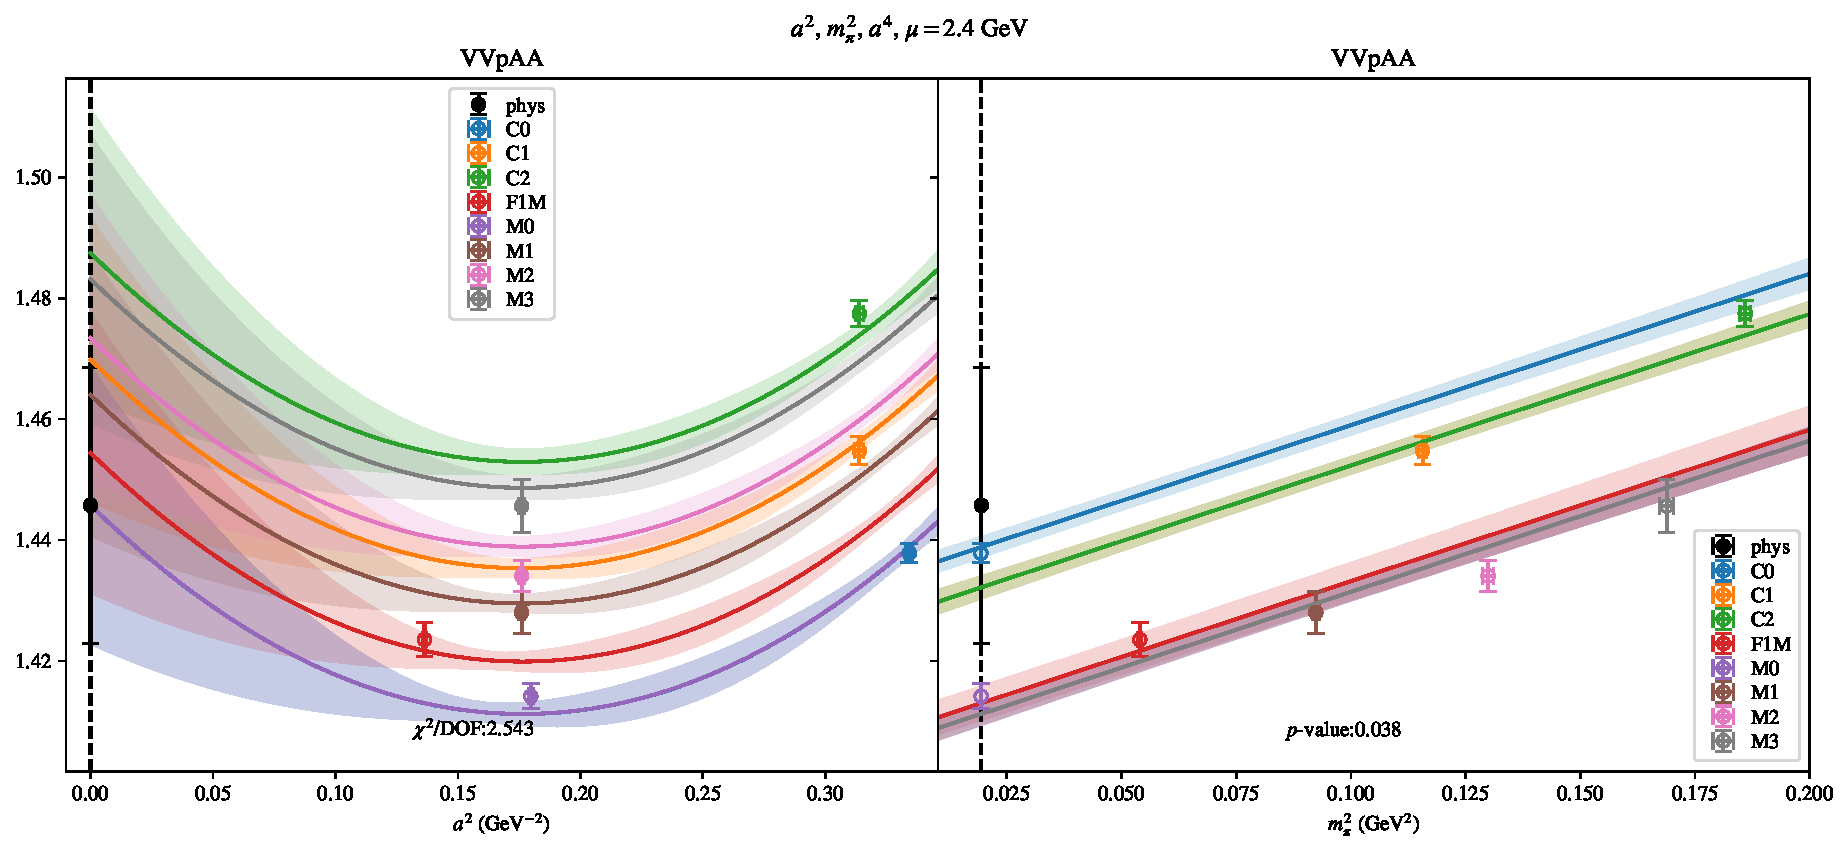
\includepdf[link, pages=-]{VVpAA/SUSY/bag_a2a4m2_24.pdf}
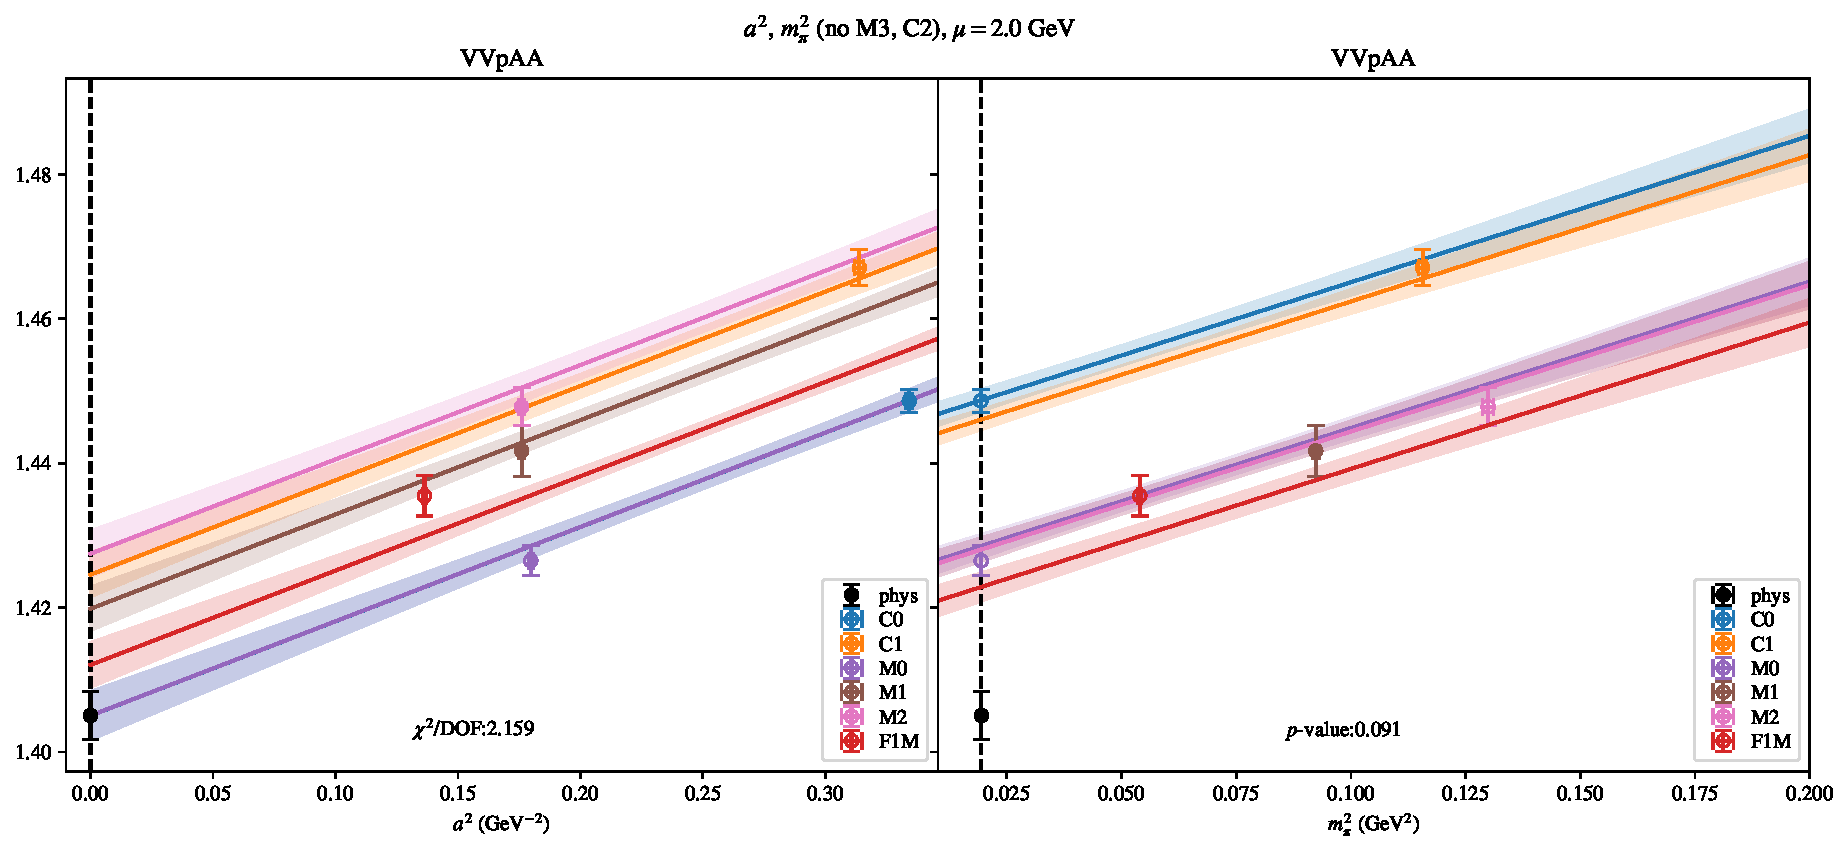
\includepdf[link, pages=-]{VVpAA/SUSY/bag_a2m2mcut_20.pdf}
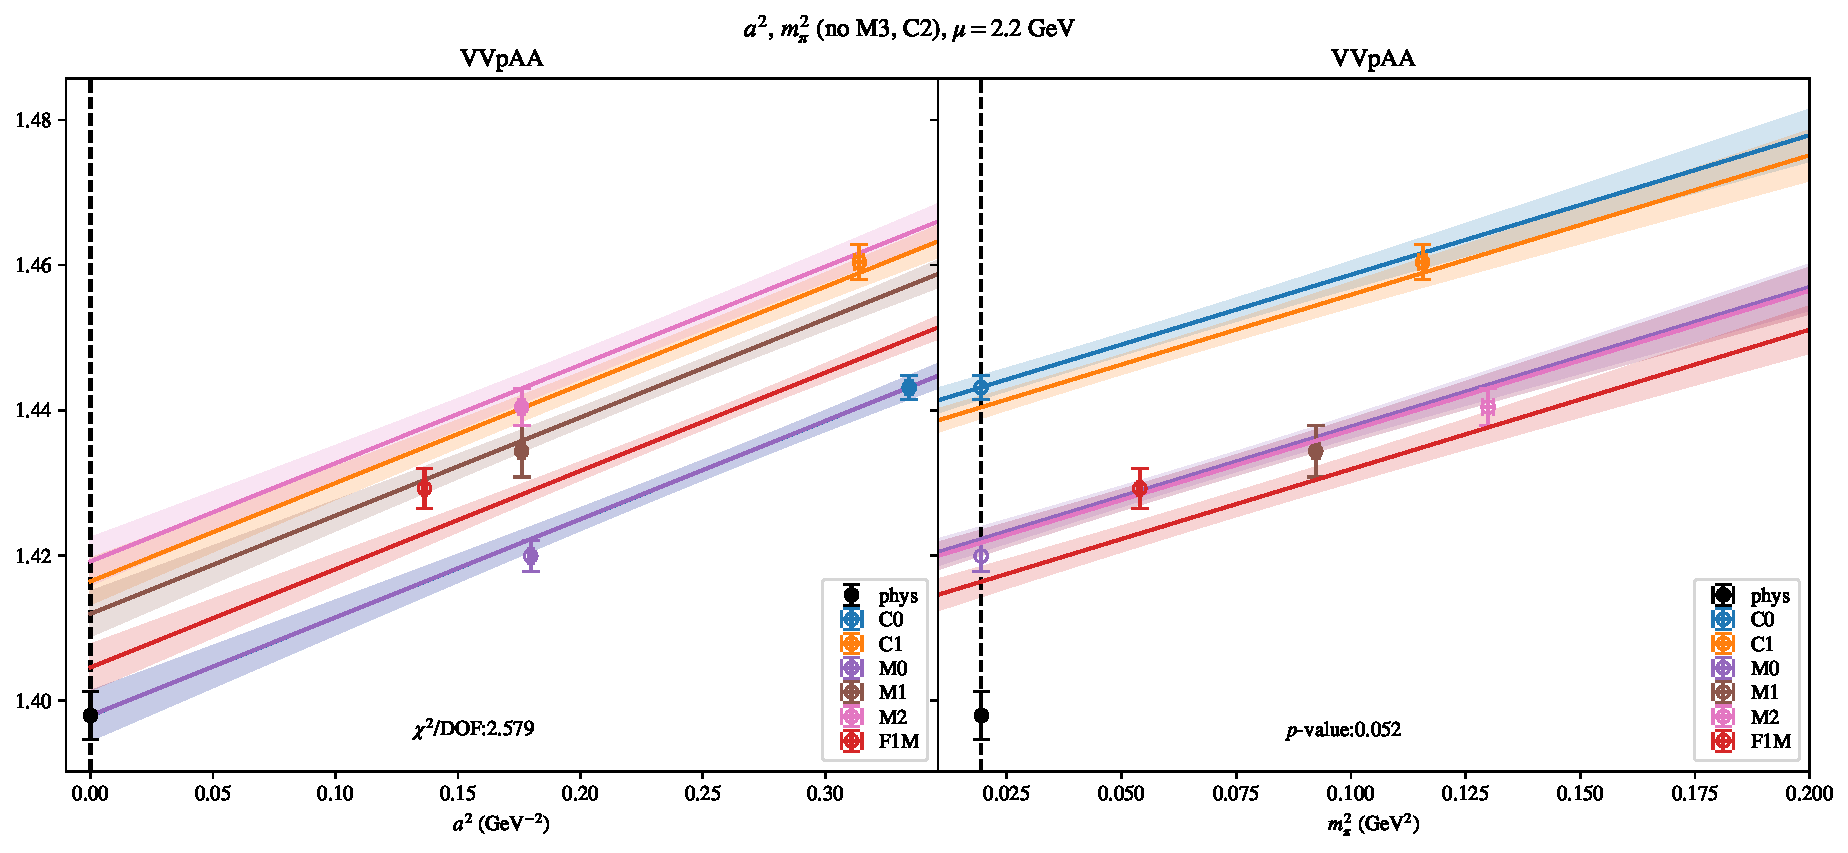
\includepdf[link, pages=-]{VVpAA/SUSY/bag_a2m2mcut_22.pdf}
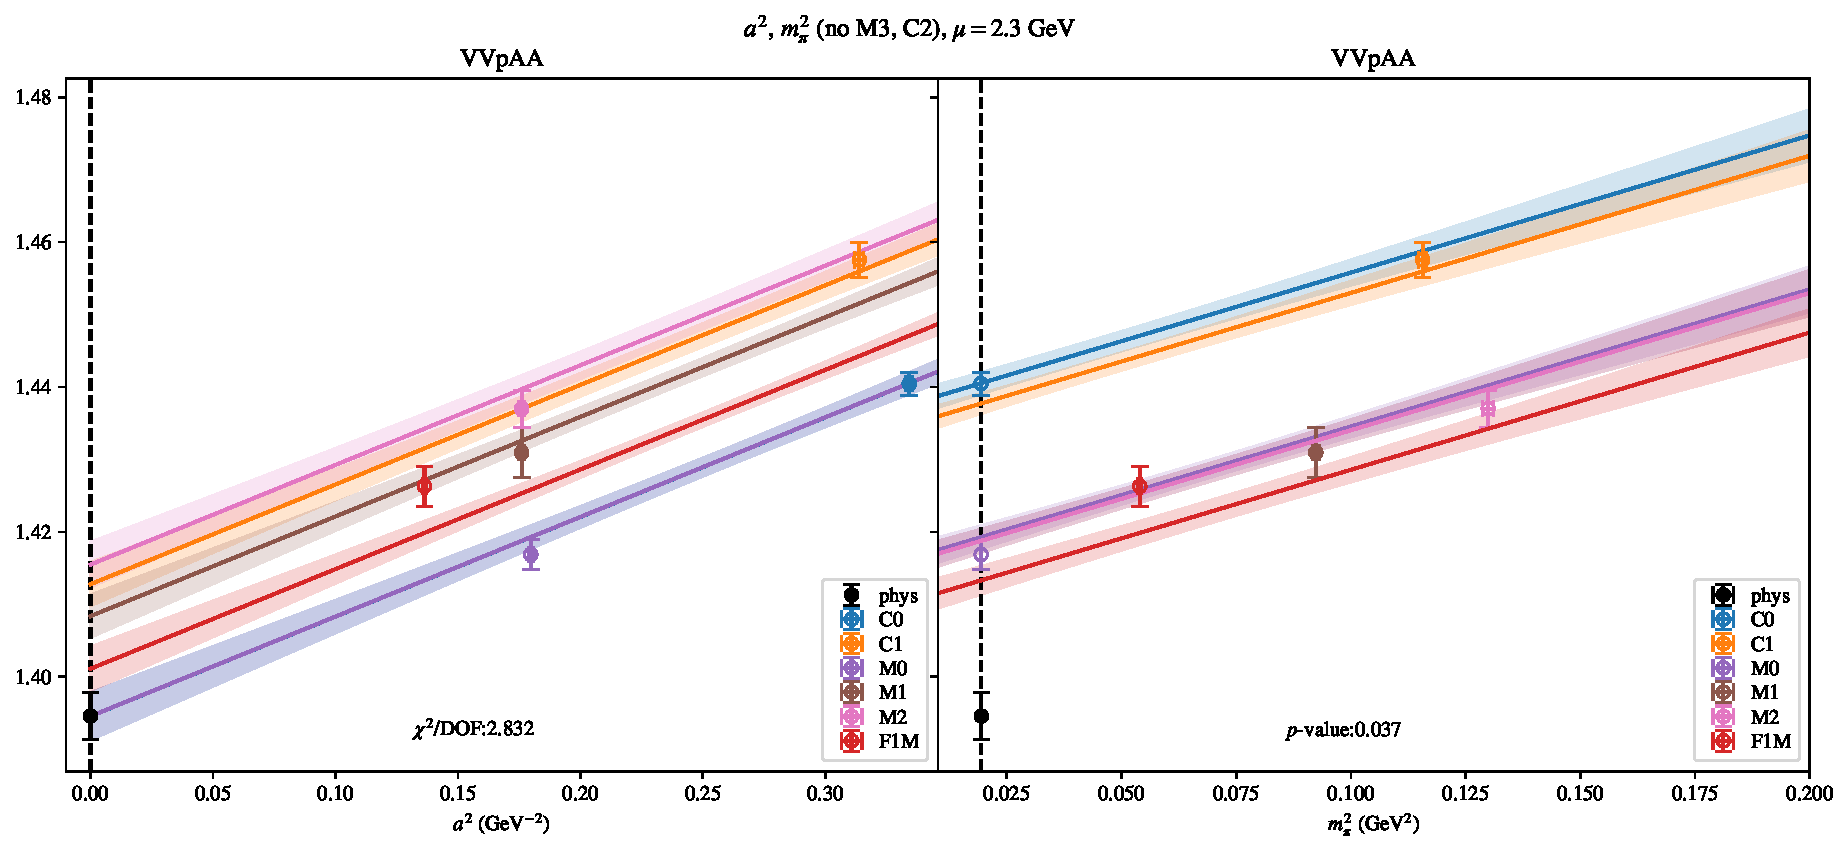
\includepdf[link, pages=-]{VVpAA/SUSY/bag_a2m2mcut_23.pdf}
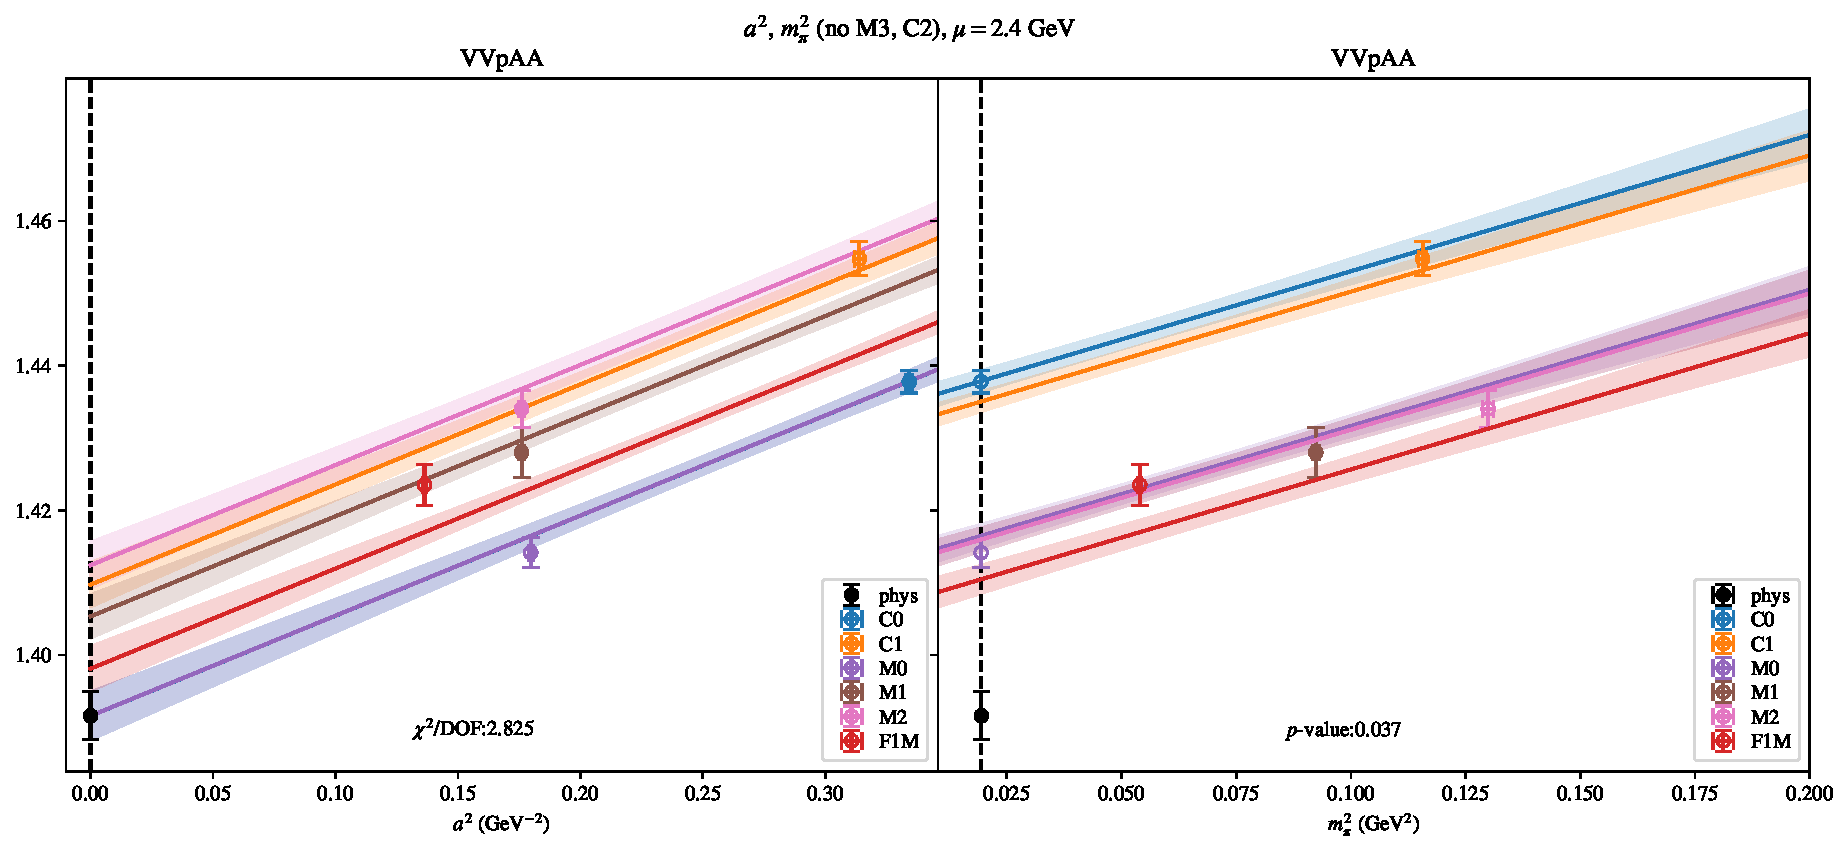
\includepdf[link, pages=-]{VVpAA/SUSY/bag_a2m2mcut_24.pdf}
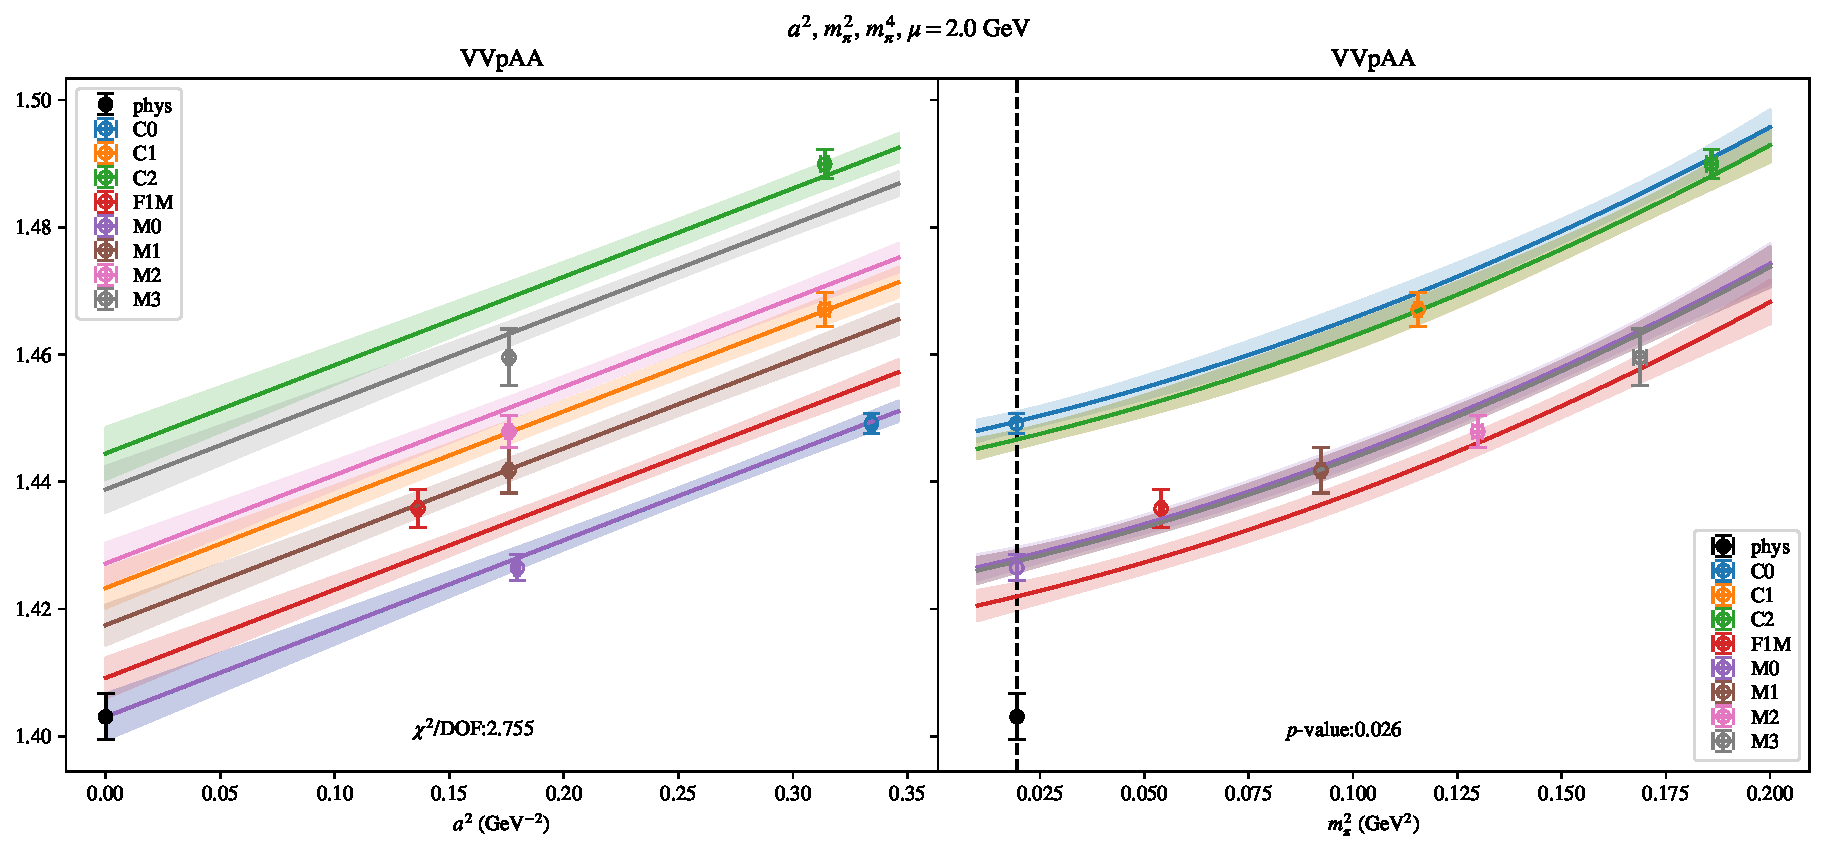
\includepdf[link, pages=-]{VVpAA/SUSY/bag_a2m2m4_20.pdf}
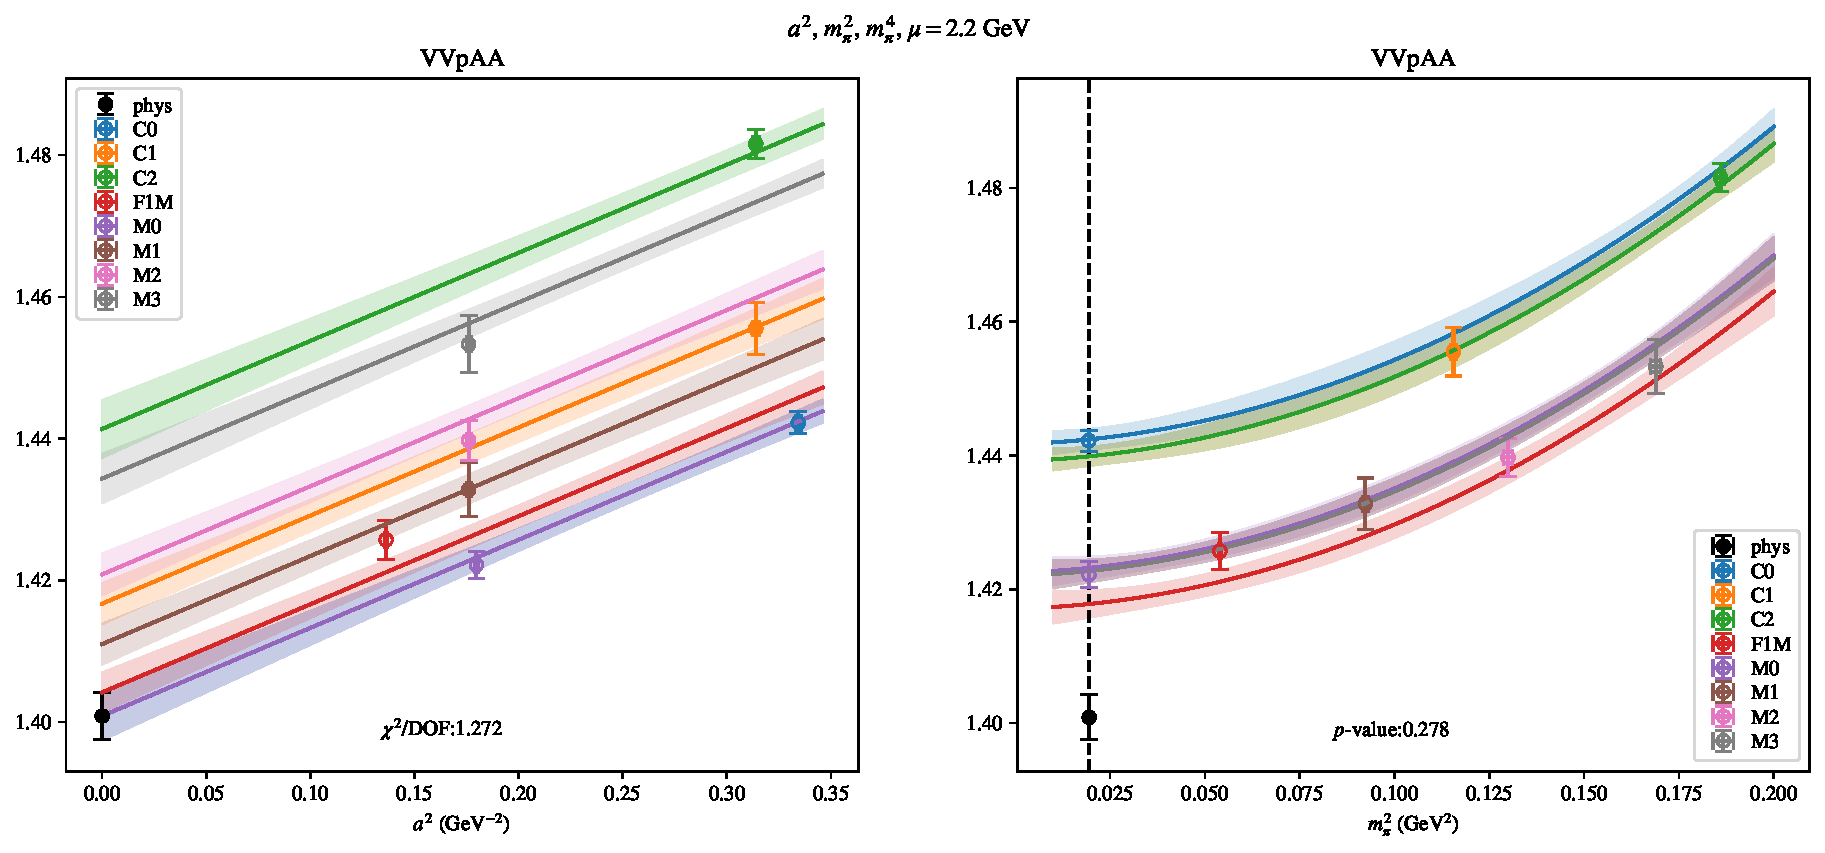
\includepdf[link, pages=-]{VVpAA/SUSY/bag_a2m2m4_22.pdf}
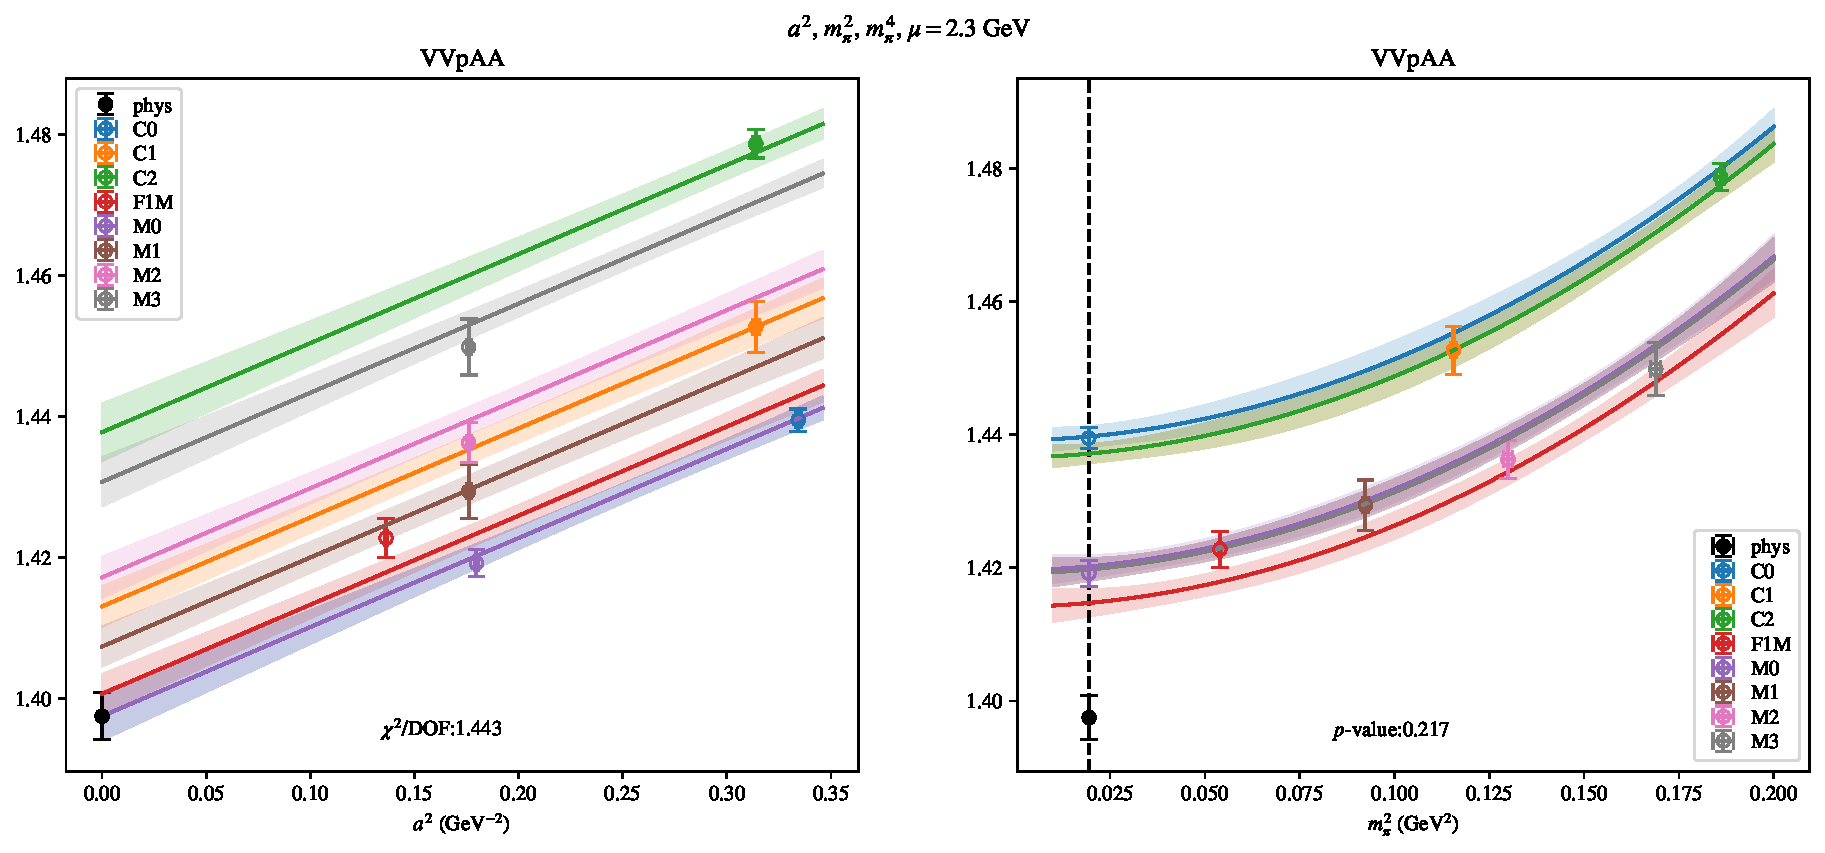
\includepdf[link, pages=-]{VVpAA/SUSY/bag_a2m2m4_23.pdf}
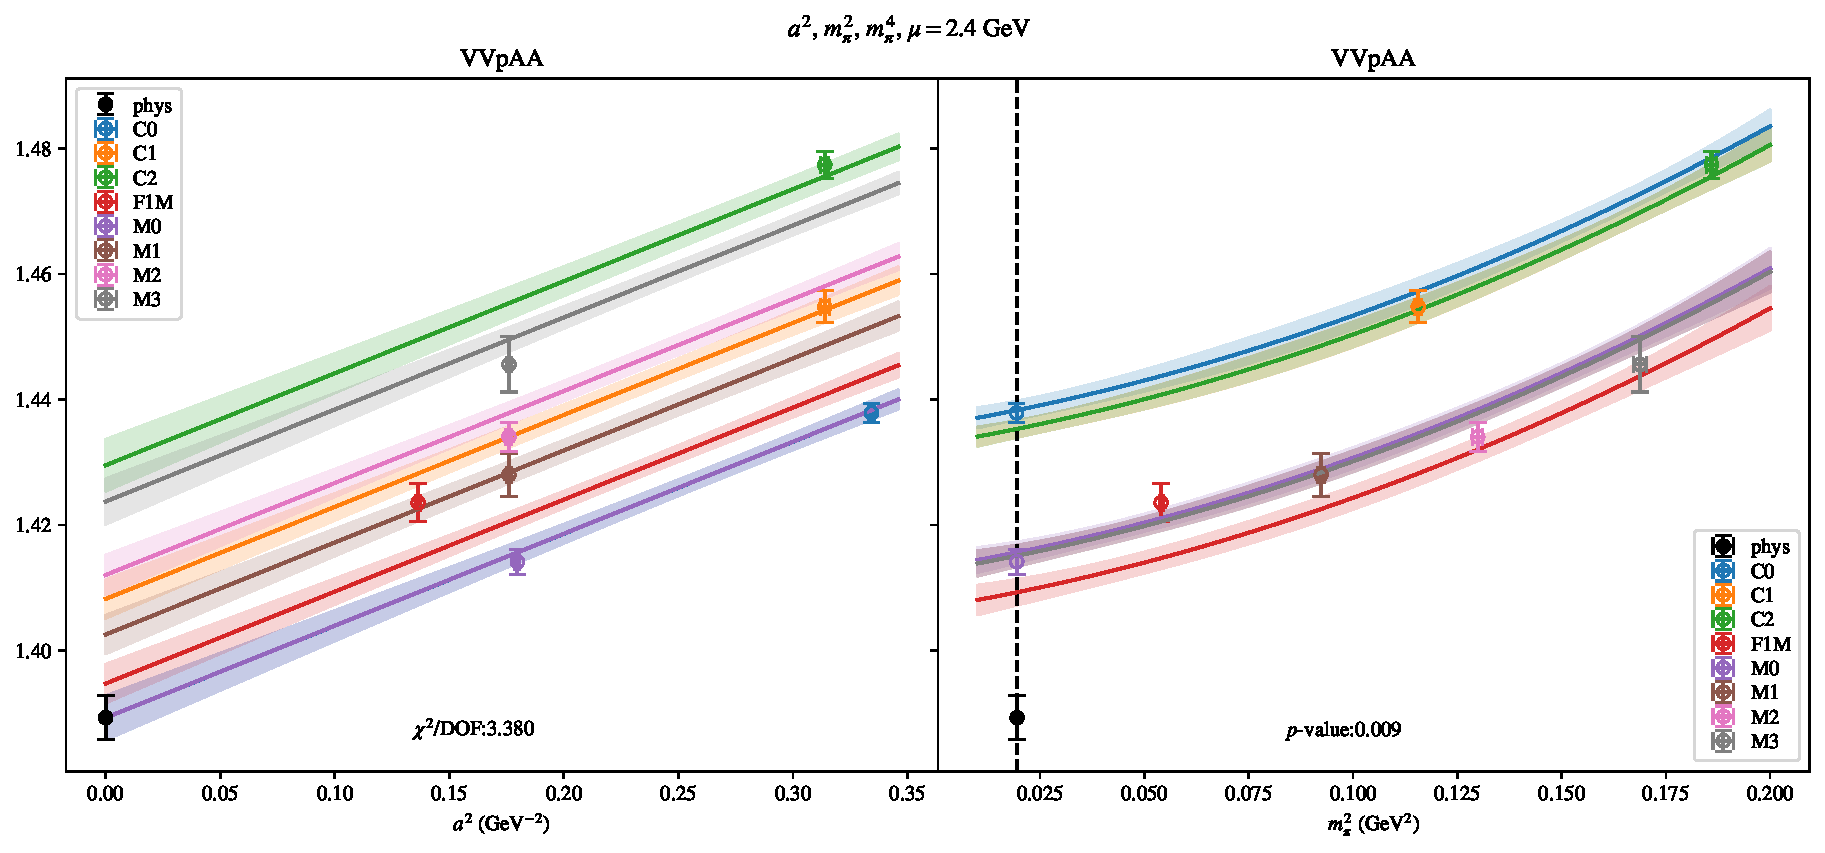
\includepdf[link, pages=-]{VVpAA/SUSY/bag_a2m2m4_24.pdf}
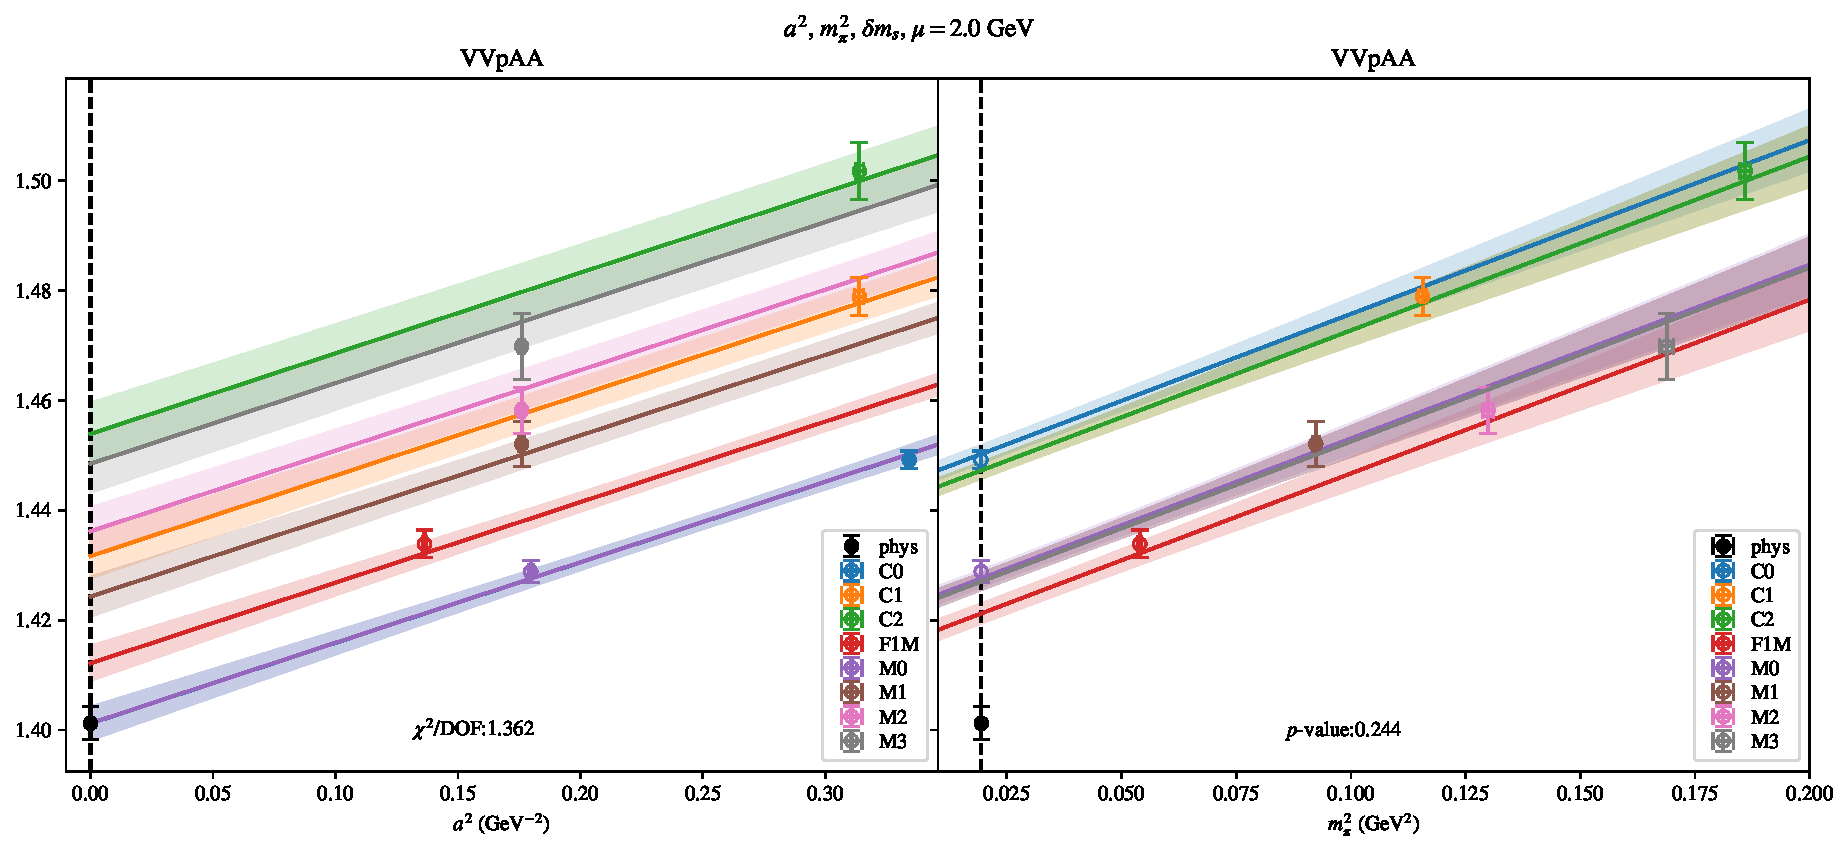
\includepdf[link, pages=-]{VVpAA/SUSY/bag_a2m2delm_20.pdf}
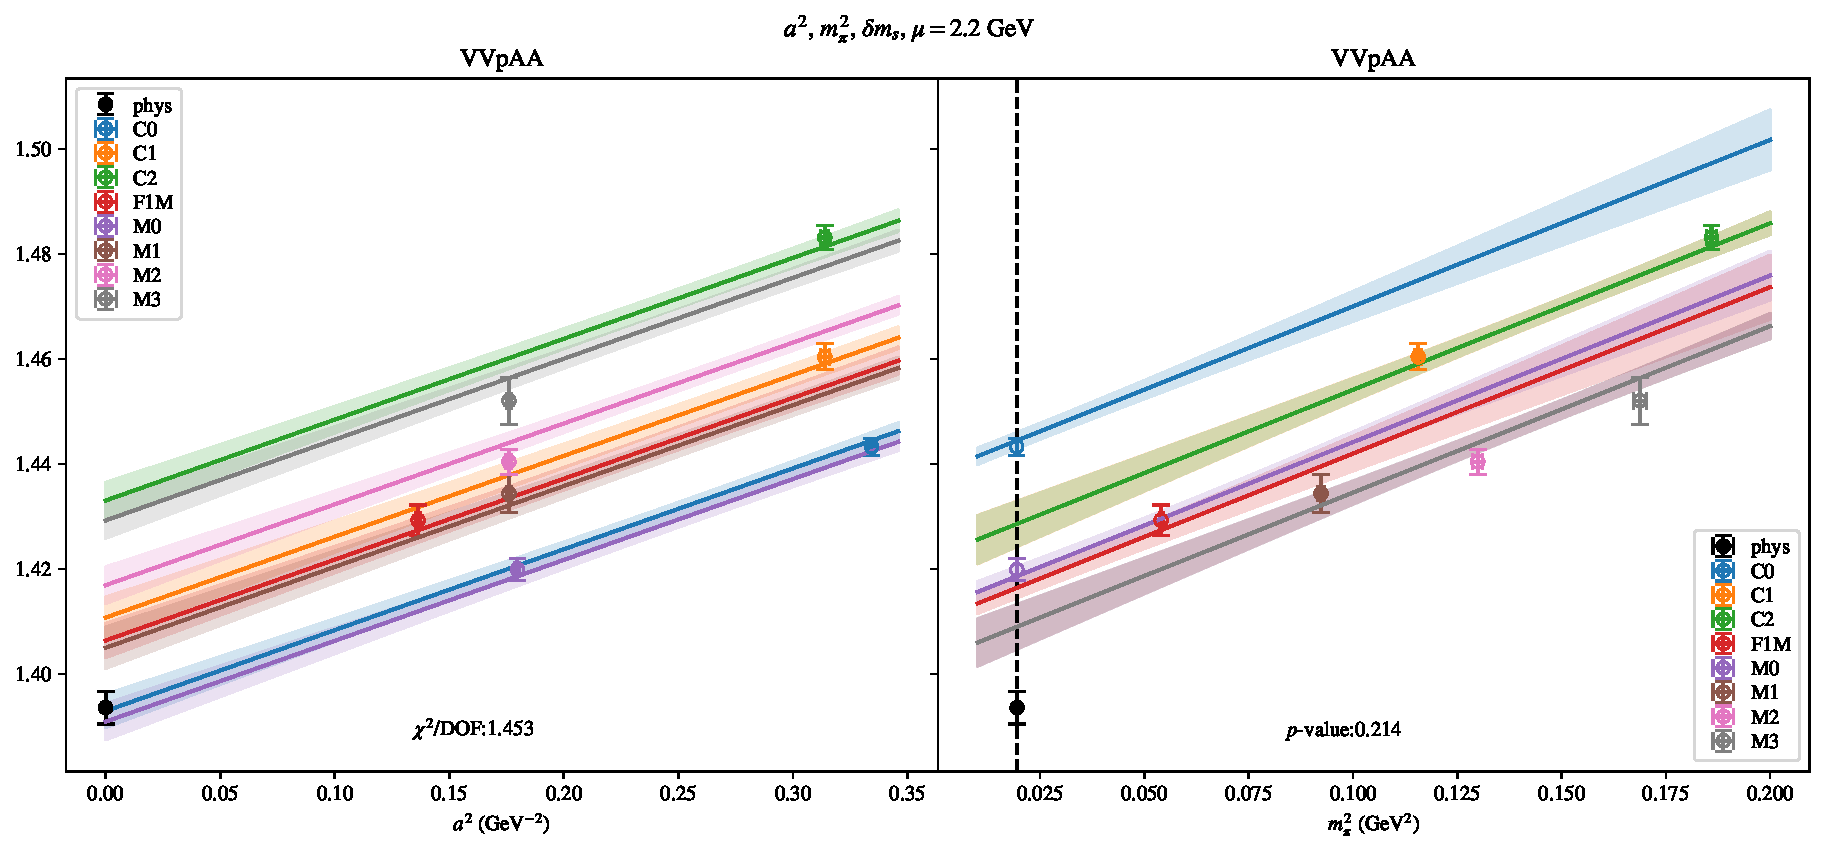
\includepdf[link, pages=-]{VVpAA/SUSY/bag_a2m2delm_22.pdf}
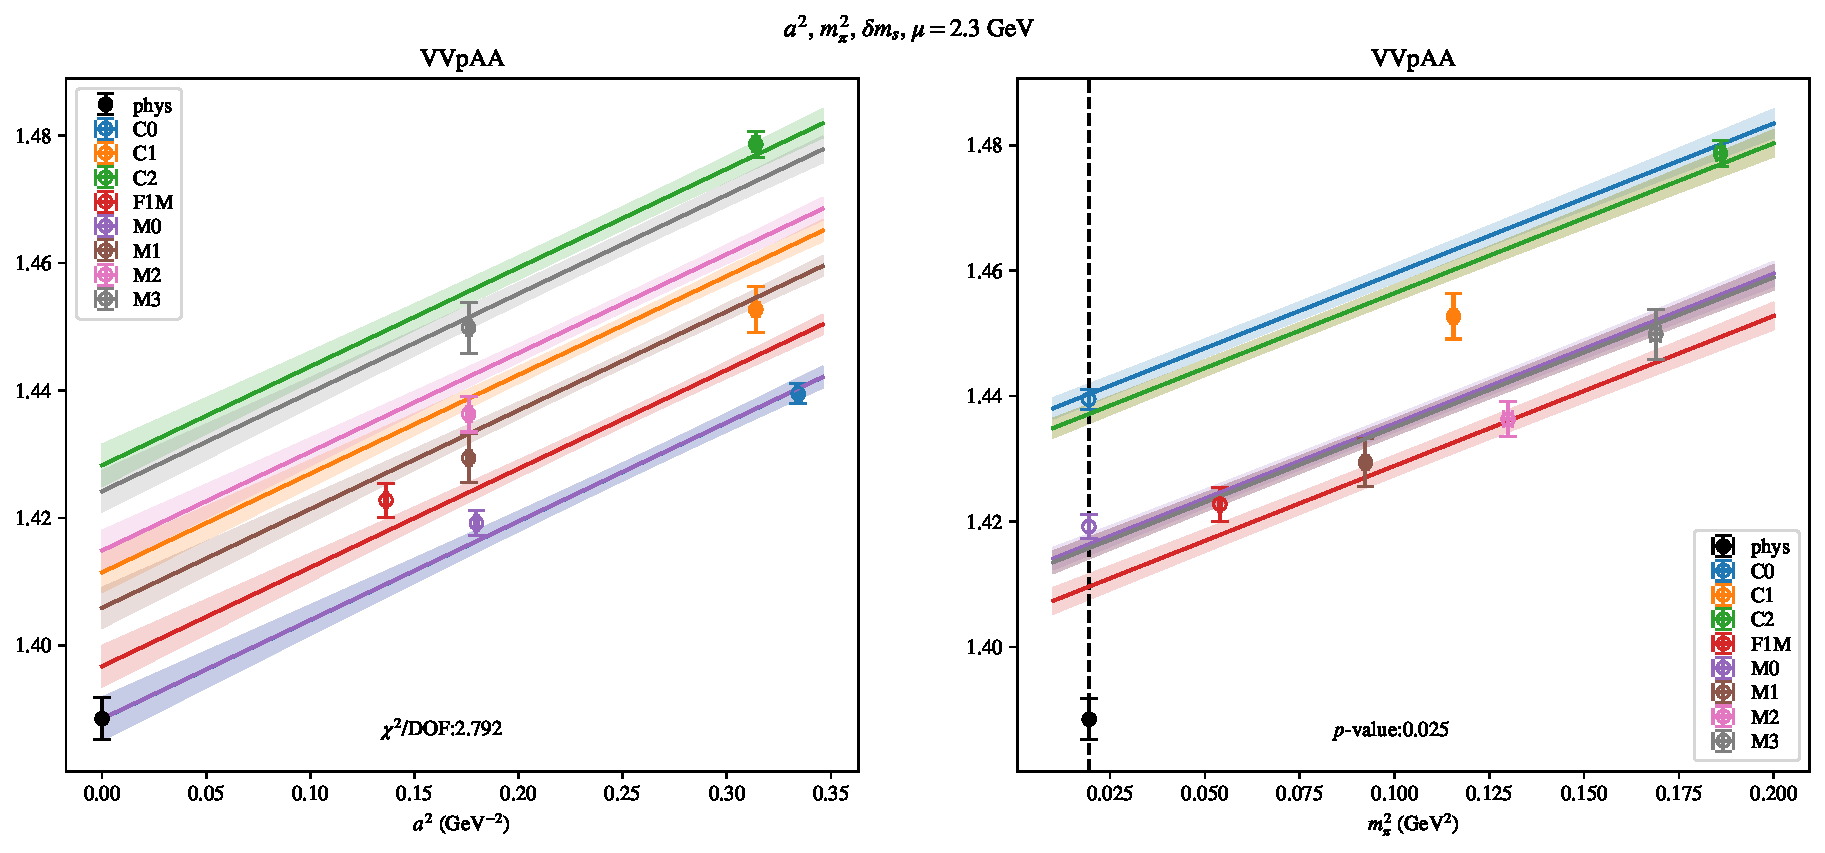
\includepdf[link, pages=-]{VVpAA/SUSY/bag_a2m2delm_23.pdf}
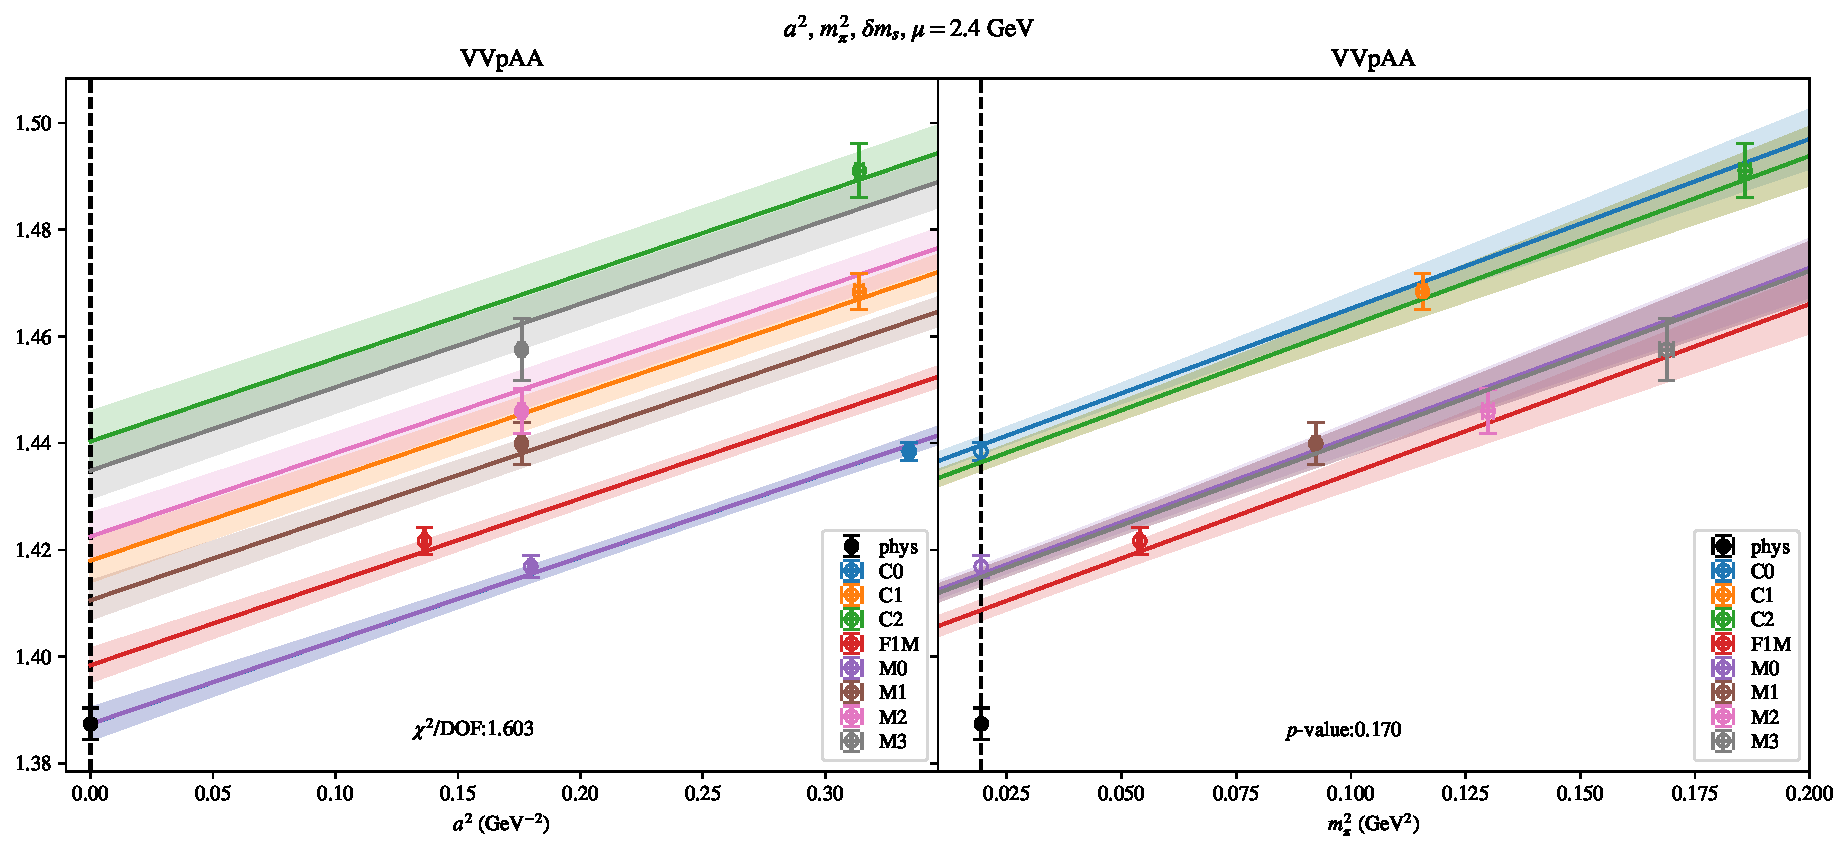
\includepdf[link, pages=-]{VVpAA/SUSY/bag_a2m2delm_24.pdf}
\clearpage
\section{$\mathcal{B}_2$}
\begin{table}[h!]
\begin{center}
\begin{tabular}{|c|c|c|c|c|c|c|}
\hline
$\mu$ (GeV) & $a^2$, $m_\pi^2$& $a^2$, $m_\pi^2$ (no C)& $a^2$, $m_\pi^2$, $a^4$& $a^2$, $m_\pi^2$ (no M3, C2)& $a^2$, $m_\pi^2$, $m_\pi^4$& $a^2$, $m_\pi^2$, $\delta m_s$\\
\hline
2.0& \hyperlink{VVmAA/SUSY/bag_a2m2_20.pdf.1}{\textbf{-0.9282(27)}: 0.635 (0.673)} & \hyperlink{VVmAA/SUSY/bag_a2m2noC_20.pdf.1}{\textbf{-0.931(10)}: 0.692 (0.501)} & \hyperlink{VVmAA/SUSY/bag_a2a4m2_20.pdf.1}{\textbf{-0.928(16)}: 0.793 (0.53)} & \hyperlink{VVmAA/SUSY/bag_a2m2mcut_20.pdf.1}{\textbf{-0.9277(24)}: 0.576 (0.631)} & \hyperlink{VVmAA/SUSY/bag_a2m2m4_20.pdf.1}{\textbf{-0.9271(26)}: 0.41 (0.802)} & \hyperlink{VVmAA/SUSY/bag_a2m2delm_20.pdf.1}{\textbf{-0.9282(30)}: 0.793 (0.529)}\\
2.2& \hyperlink{VVmAA/SUSY/bag_a2m2_22.pdf.1}{\textbf{-0.9078(21)}: 1.694 (0.132)} & \hyperlink{VVmAA/SUSY/bag_a2m2noC_22.pdf.1}{\textbf{-0.9179(94)}: 0.896 (0.408)} & \hyperlink{VVmAA/SUSY/bag_a2a4m2_22.pdf.1}{\textbf{-0.911(15)}: 2.108 (0.077)} & \hyperlink{VVmAA/SUSY/bag_a2m2mcut_22.pdf.1}{\textbf{-0.9076(20)}: 1.712 (0.162)} & \hyperlink{VVmAA/SUSY/bag_a2m2m4_22.pdf.1}{\textbf{-0.9066(21)}: 1.378 (0.239)} & \hyperlink{VVmAA/SUSY/bag_a2m2delm_22.pdf.1}{\textbf{-0.9074(23)}: 2.028 (0.088)}\\
2.3& \hyperlink{VVmAA/SUSY/bag_a2m2_23.pdf.1}{\textbf{-0.8985(19)}: 2.537 (0.026)} & \hyperlink{VVmAA/SUSY/bag_a2m2noC_23.pdf.1}{\textbf{-0.9113(91)}: 1.266 (0.282)} & \hyperlink{VVmAA/SUSY/bag_a2a4m2_23.pdf.1}{\textbf{-0.902(14)}: 3.155 (0.013)} & \hyperlink{VVmAA/SUSY/bag_a2m2mcut_23.pdf.1}{\textbf{-0.8985(18)}: 2.754 (0.041)} & \hyperlink{VVmAA/SUSY/bag_a2m2m4_23.pdf.1}{\textbf{-0.8972(20)}: 2.34 (0.053)} & \hyperlink{VVmAA/SUSY/bag_a2m2delm_23.pdf.1}{\textbf{-0.8980(21)}: 2.995 (0.017)}\\
2.4& \hyperlink{VVmAA/SUSY/bag_a2m2_24.pdf.1}{\textbf{-0.8904(18)}: 3.176 (0.007)} & \hyperlink{VVmAA/SUSY/bag_a2m2noC_24.pdf.1}{\textbf{-0.9044(89)}: 1.543 (0.214)} & \hyperlink{VVmAA/SUSY/bag_a2a4m2_24.pdf.1}{\textbf{-0.894(14)}: 3.957 (0.003)} & \hyperlink{VVmAA/SUSY/bag_a2m2mcut_24.pdf.1}{\textbf{-0.8905(18)}: 3.509 (0.015)} & \hyperlink{VVmAA/SUSY/bag_a2m2m4_24.pdf.1}{\textbf{-0.8891(19)}: 3.088 (0.015)} & \hyperlink{VVmAA/SUSY/bag_a2m2delm_24.pdf.1}{\textbf{-0.8899(20)}: 3.739 (0.005)}\\
\hline
\end{tabular}
\caption{Physical point value from chiral and continuum extrapolation at renormalisation scale $\mu$. Entries are \textbf{value(error)}: $\chi^2/\text{DOF}$ ($p$-value).}
\end{center}
\end{table}
\begin{table}[h!]
\begin{center}
\begin{tabular}{|c c|c|c|c|c|c|c|}
\hline
$\mu$ (GeV) &  & $a^2$, $m_\pi^2$& $a^2$, $m_\pi^2$ (no C)& $a^2$, $m_\pi^2$, $a^4$& $a^2$, $m_\pi^2$ (no M3, C2)& $a^2$, $m_\pi^2$, $m_\pi^4$& $a^2$, $m_\pi^2$, $\delta m_s$\\
\hline
\multirow{3}{0.5in}{2.0} & $\alpha$ & -0.341(10)& -0.328(62)& -0.35(14)& -0.3428(95)& -0.345(10)& -0.341(11)\\
 & $\beta$ & -0.00699(30)& -0.00686(58)& -0.00699(30)& -0.00742(43)& -0.00855(96)& -0.00699(30)\\
 & $\gamma$ &  &  & 0.01(28)&  & 0.000148(76)& 0.00002(263)\\
\hline
\multirow{3}{0.5in}{2.2} & $\alpha$ & -0.3764(82)& -0.321(55)& -0.35(13)& -0.3766(79)& -0.3802(82)& -0.3779(86)\\
 & $\beta$ & -0.00672(19)& -0.00632(38)& -0.00673(19)& -0.00711(30)& -0.00823(76)& -0.00675(19)\\
 & $\gamma$ &  &  & -0.05(27)&  & 0.000138(63)& 0.0014(24)\\
\hline
\multirow{3}{0.5in}{2.3} & $\alpha$ & -0.3945(77)& -0.324(53)& -0.36(13)& -0.3940(75)& -0.3986(77)& -0.3963(79)\\
 & $\beta$ & -0.00678(17)& -0.00631(32)& -0.00679(18)& -0.00713(28)& -0.00827(74)& -0.00682(18)\\
 & $\gamma$ &  &  & -0.07(26)&  & 0.000137(62)& 0.0019(23)\\
\hline
\multirow{3}{0.5in}{2.4} & $\alpha$ & -0.4095(72)& -0.333(52)& -0.38(13)& -0.4084(72)& -0.4137(73)& -0.4114(74)\\
 & $\beta$ & -0.00675(15)& -0.00626(27)& -0.00676(16)& -0.00709(26)& -0.00820(71)& -0.00680(16)\\
 & $\gamma$ &  &  & -0.06(26)&  & 0.000132(61)& 0.0021(22)\\
\hline
\end{tabular}
\caption{Fit values of coefficients in $Q = Q_{phys} + \mathbf{\alpha} a^2 + \mathbf{\beta}\left(\frac{m_\pi^2}{f_\pi^2}-\frac{m_{\pi,PDG}^2}{f_\pi^2}\right) + \gamma(\ldots)$}
\end{center}
\end{table}
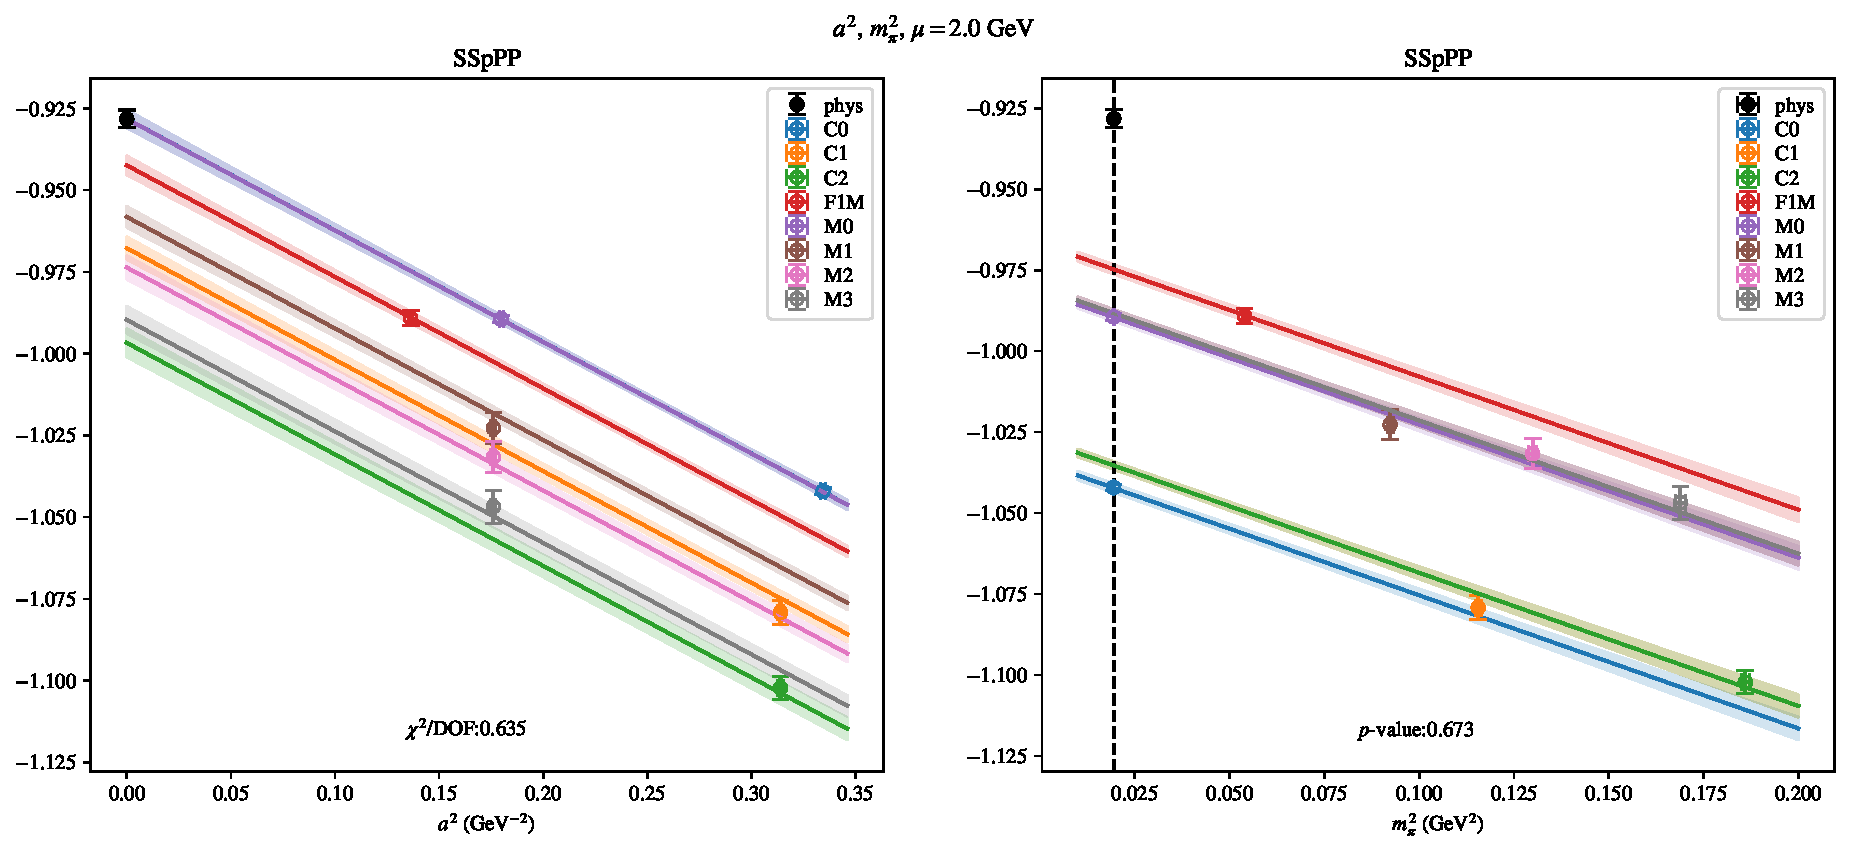
\includepdf[link, pages=-]{VVmAA/SUSY/bag_a2m2_20.pdf}
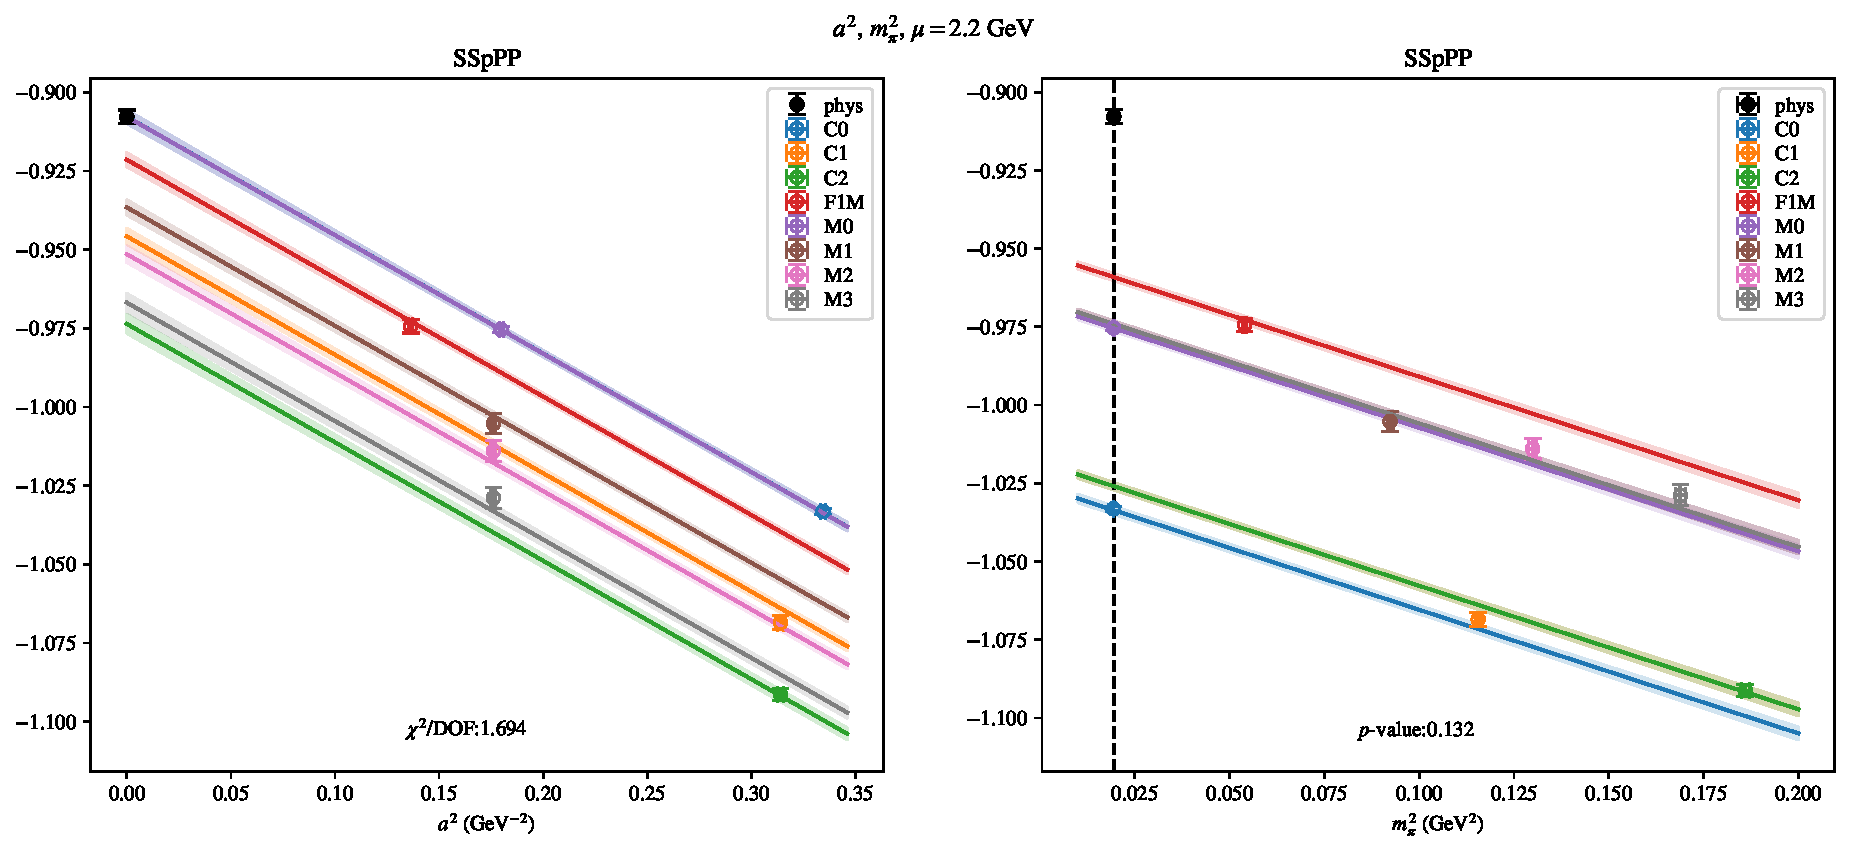
\includepdf[link, pages=-]{VVmAA/SUSY/bag_a2m2_22.pdf}
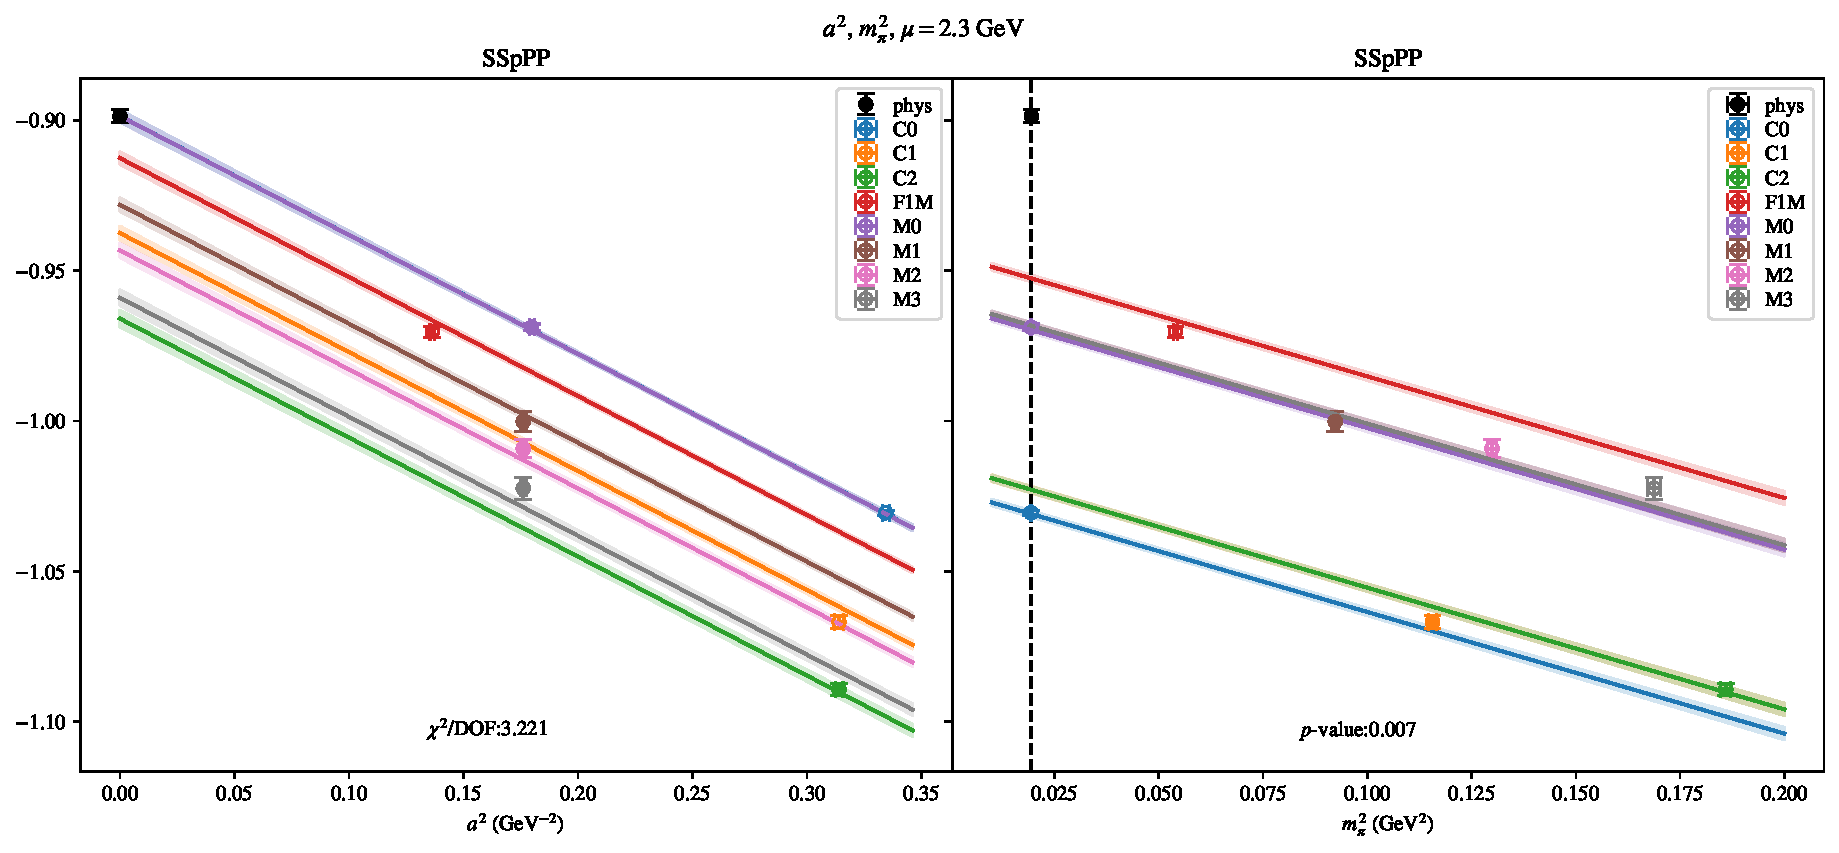
\includepdf[link, pages=-]{VVmAA/SUSY/bag_a2m2_23.pdf}
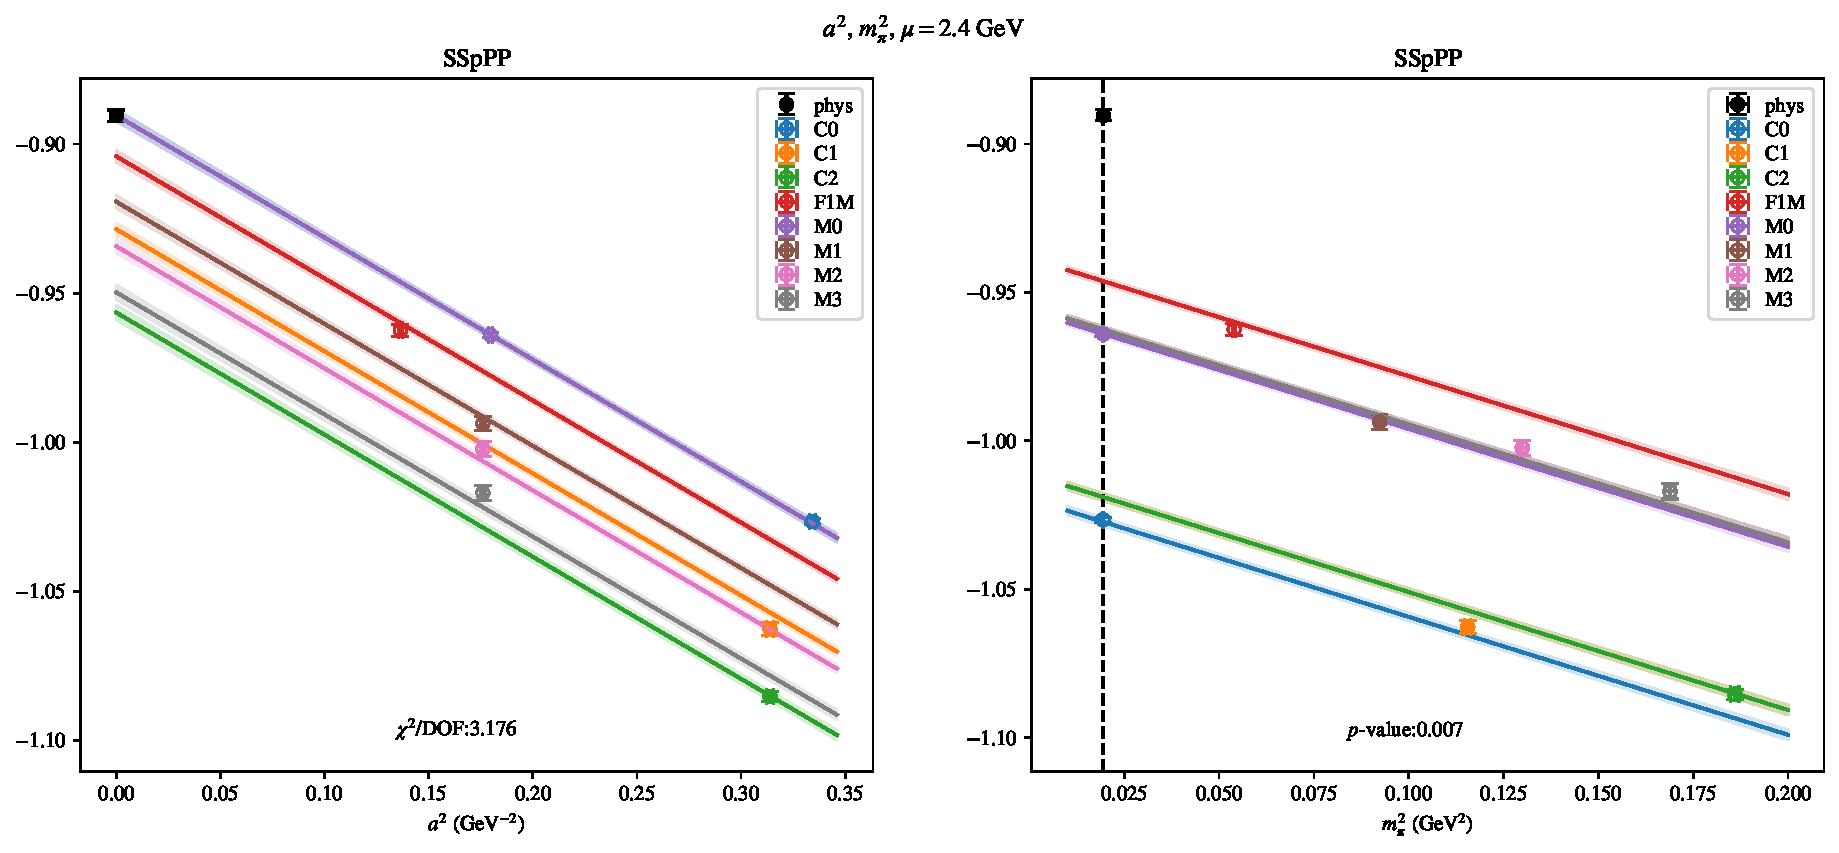
\includepdf[link, pages=-]{VVmAA/SUSY/bag_a2m2_24.pdf}
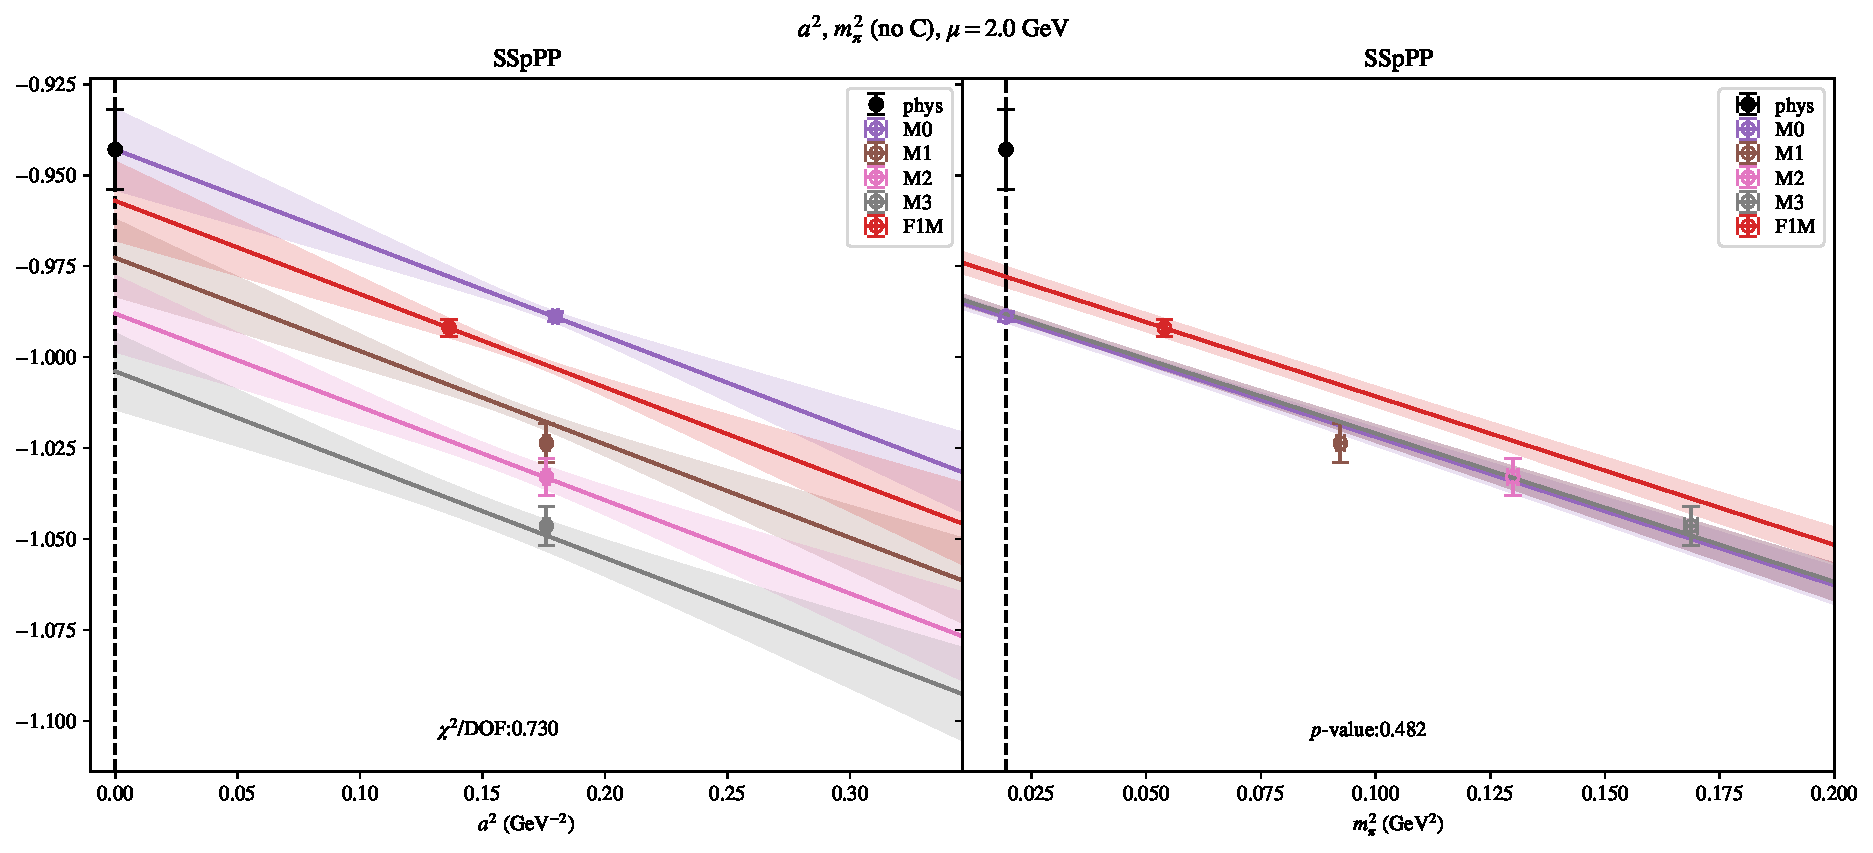
\includepdf[link, pages=-]{VVmAA/SUSY/bag_a2m2noC_20.pdf}
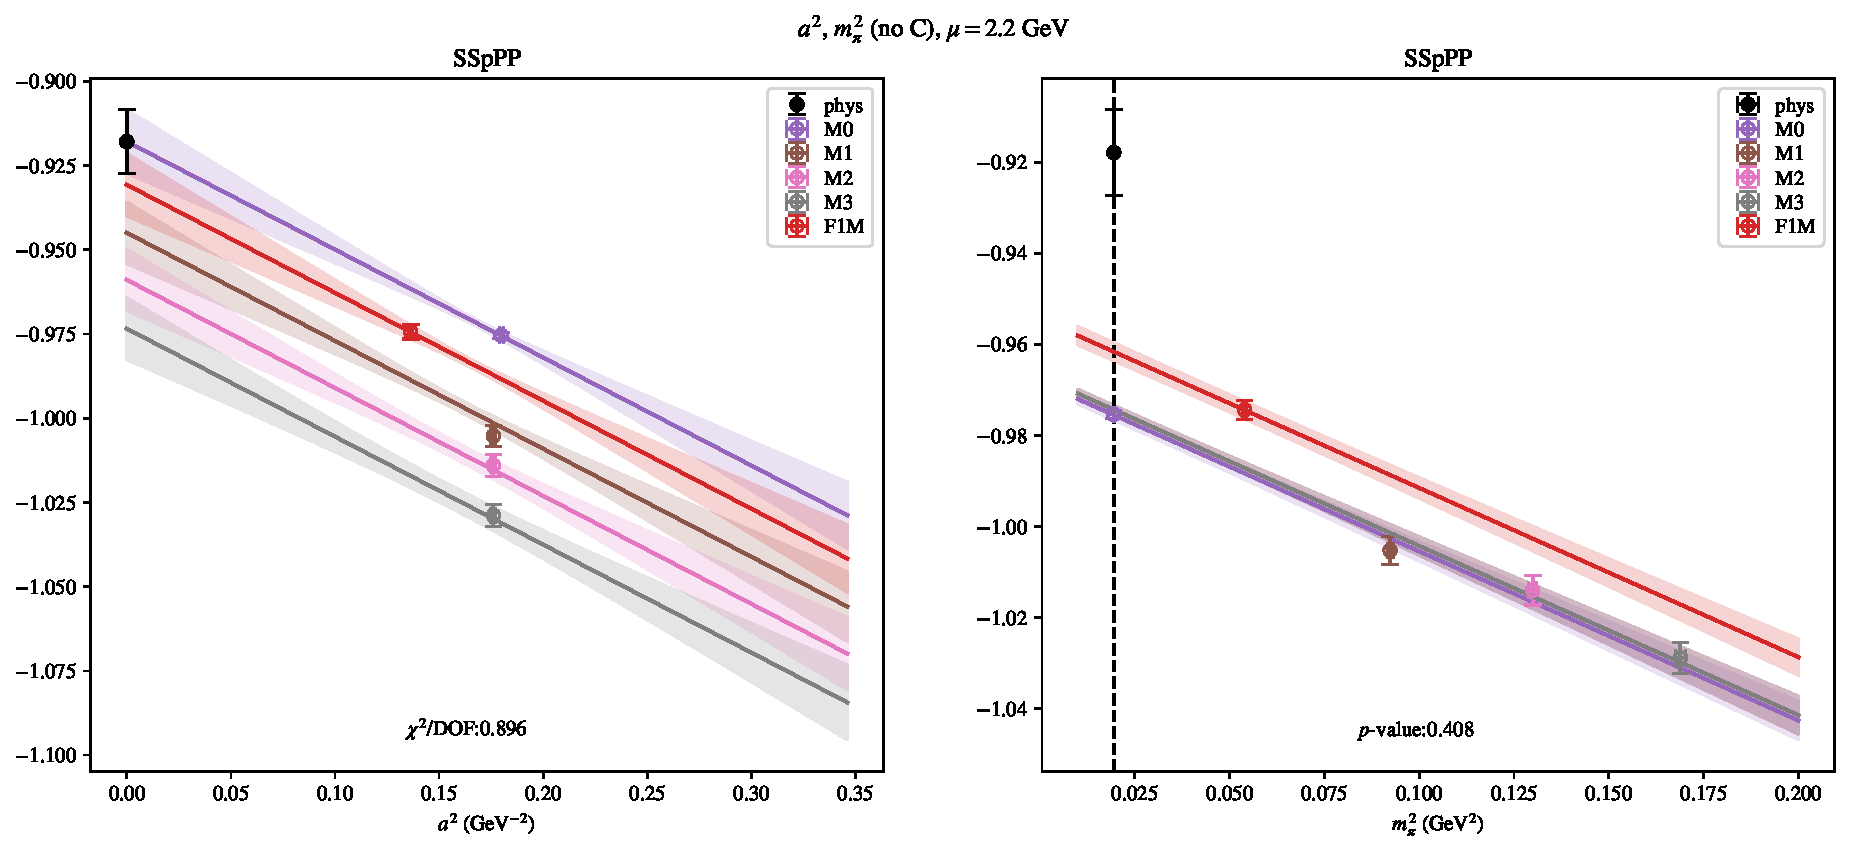
\includepdf[link, pages=-]{VVmAA/SUSY/bag_a2m2noC_22.pdf}
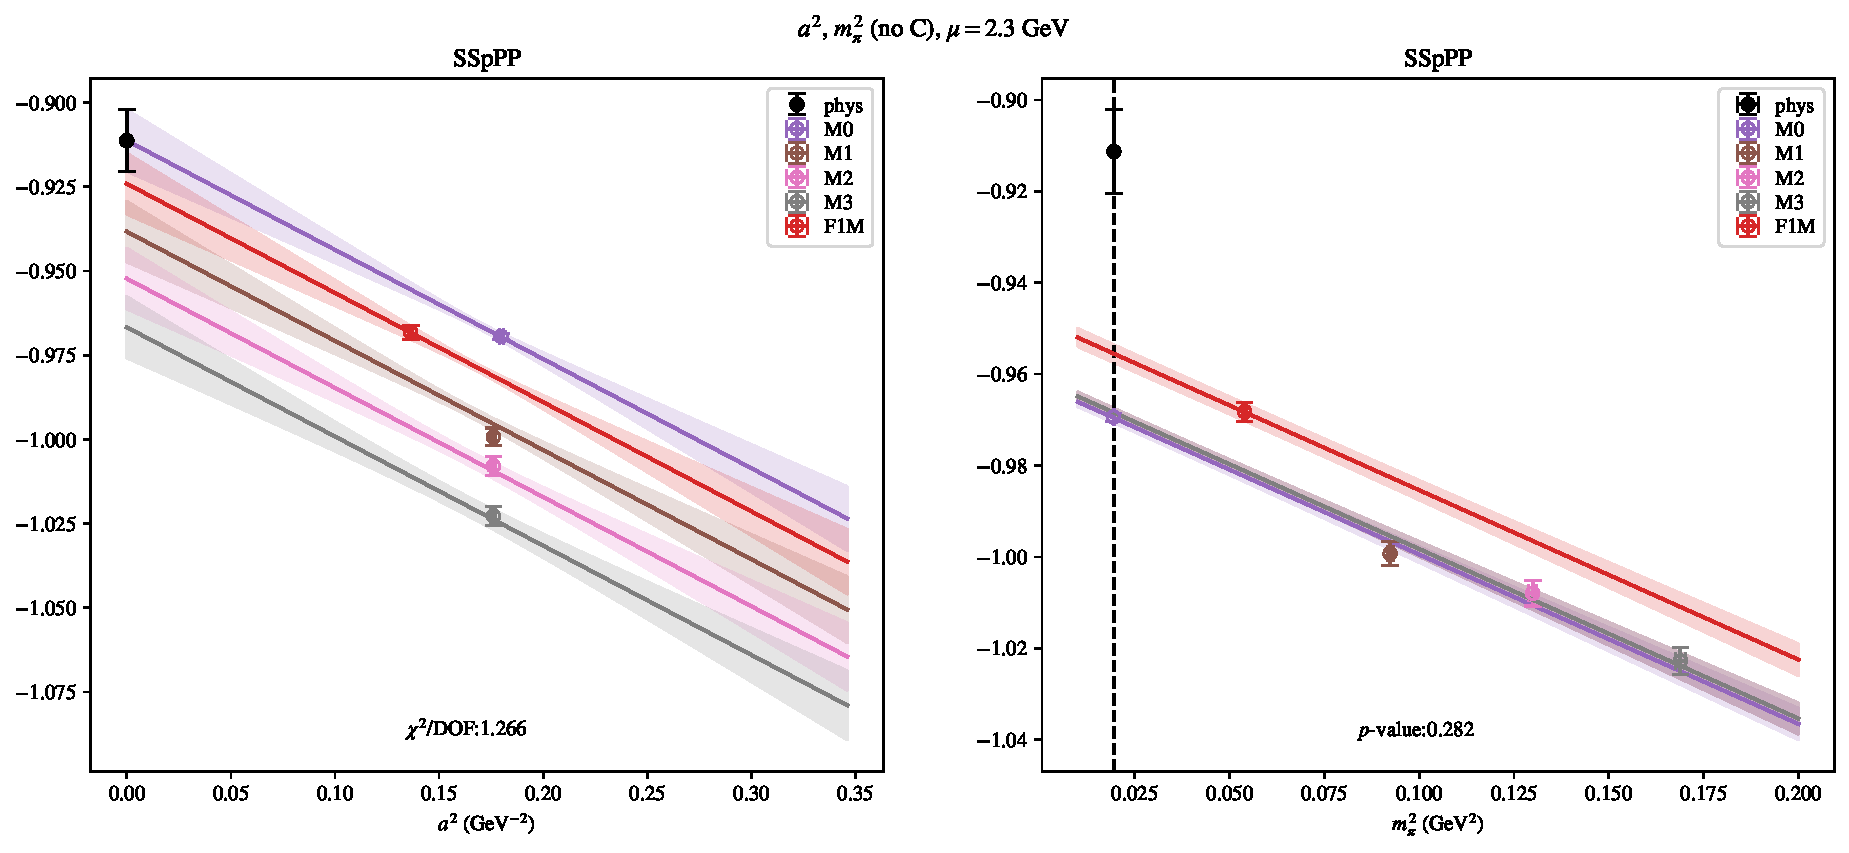
\includepdf[link, pages=-]{VVmAA/SUSY/bag_a2m2noC_23.pdf}
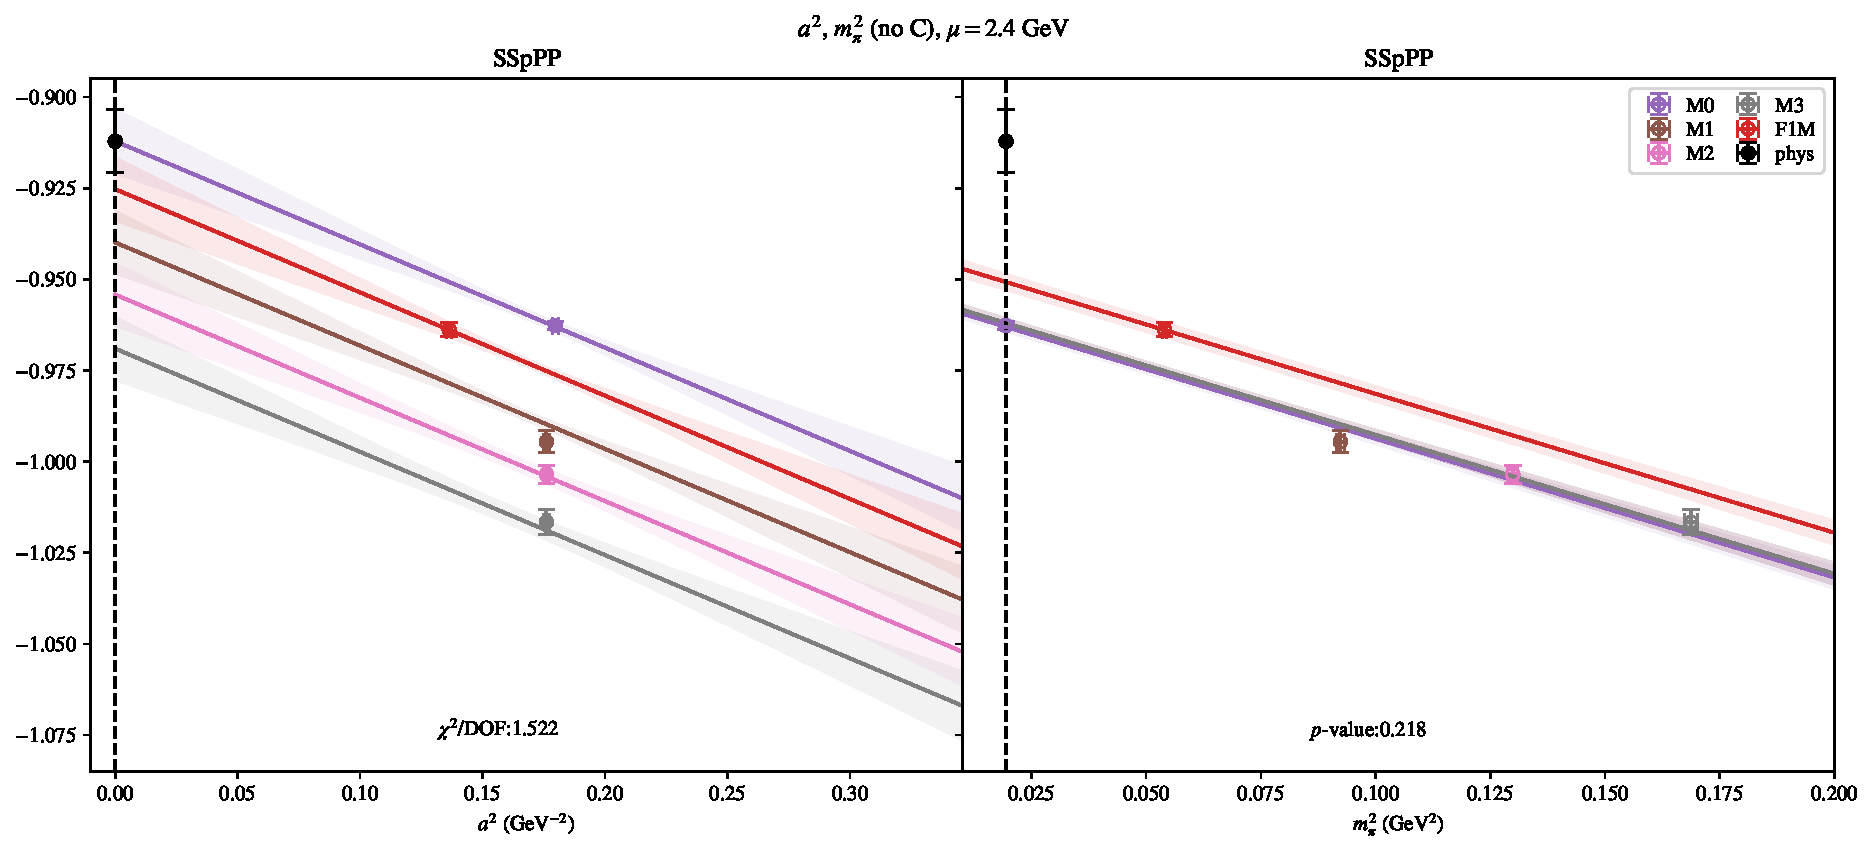
\includepdf[link, pages=-]{VVmAA/SUSY/bag_a2m2noC_24.pdf}
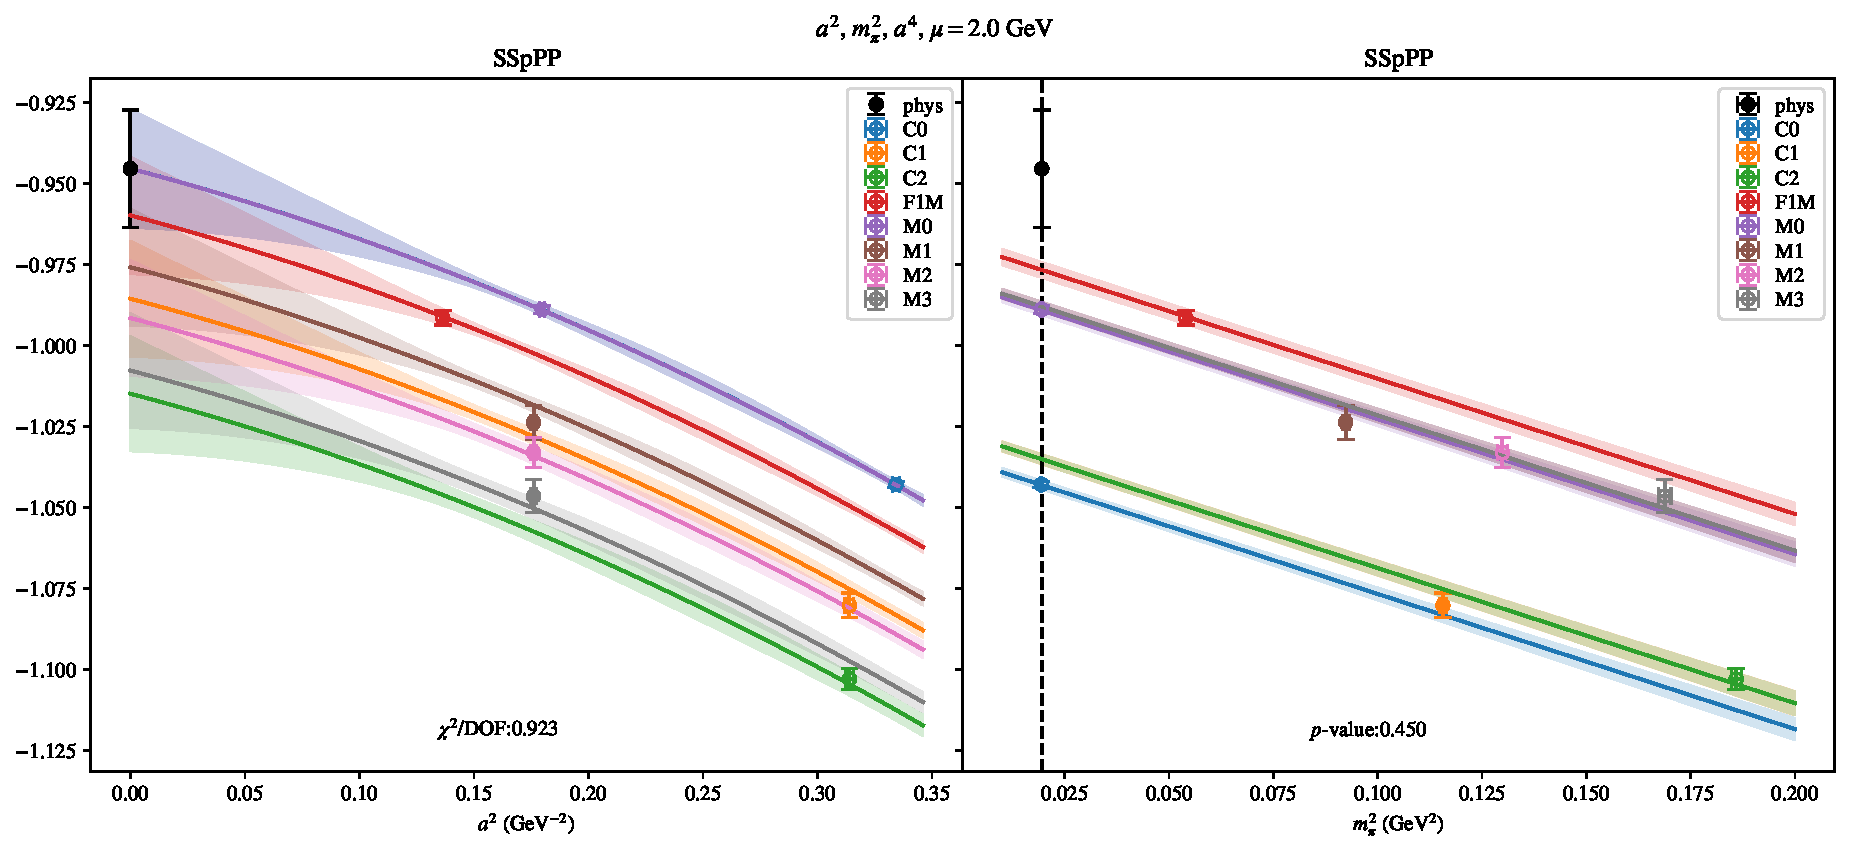
\includepdf[link, pages=-]{VVmAA/SUSY/bag_a2a4m2_20.pdf}
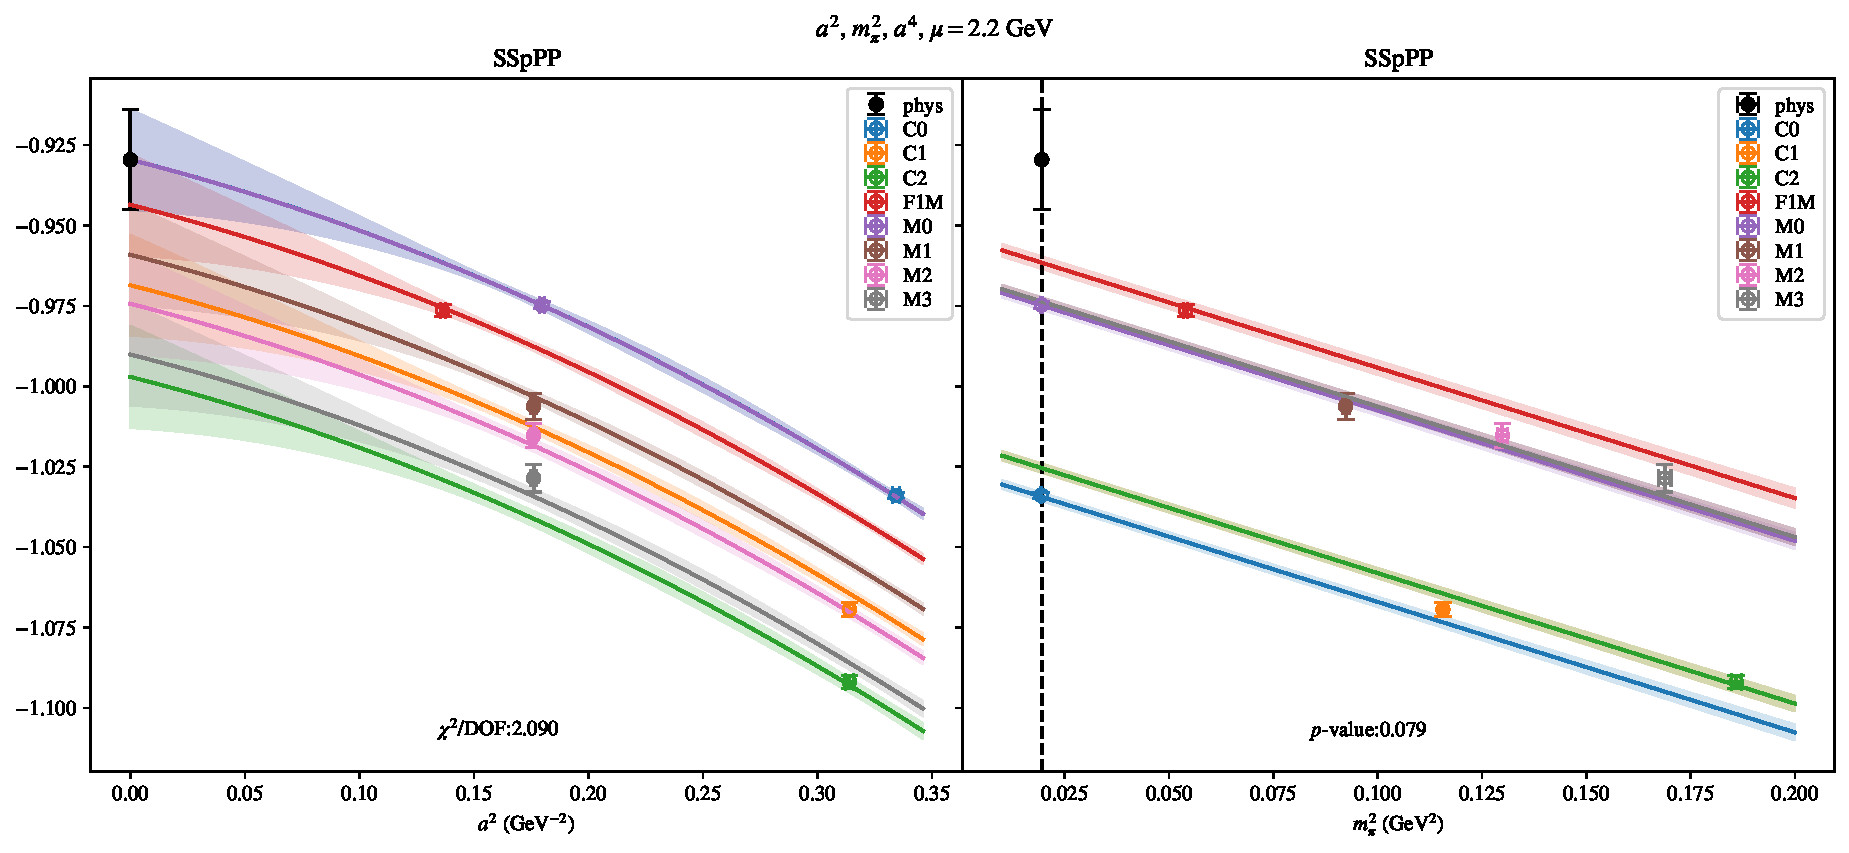
\includepdf[link, pages=-]{VVmAA/SUSY/bag_a2a4m2_22.pdf}
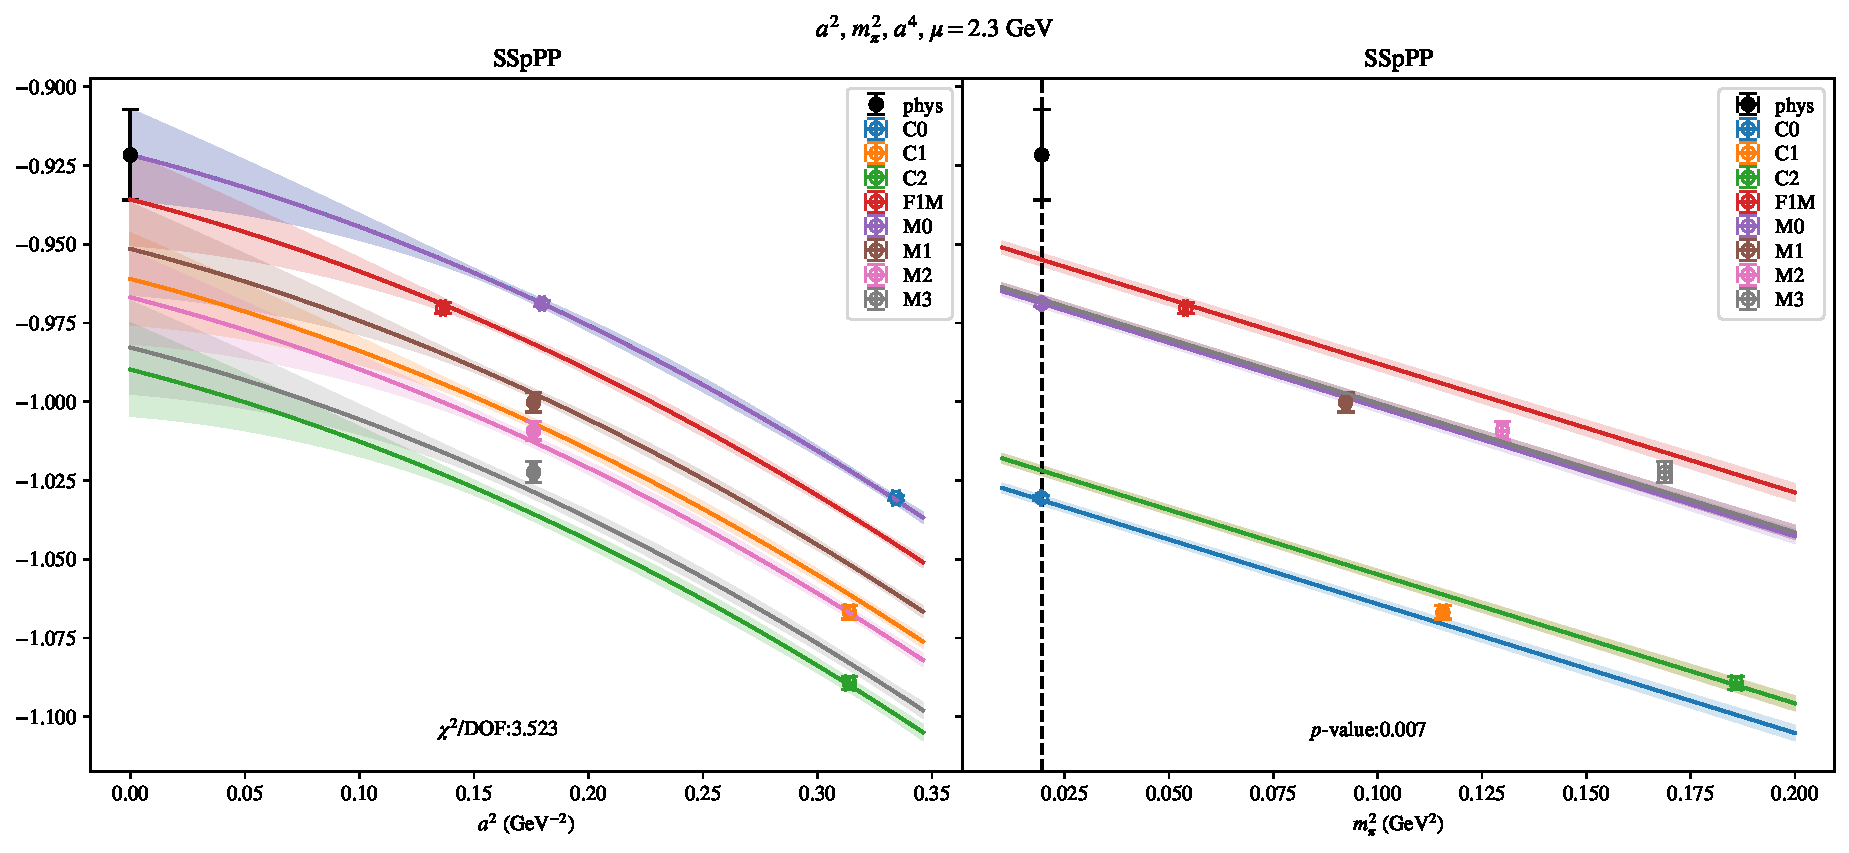
\includepdf[link, pages=-]{VVmAA/SUSY/bag_a2a4m2_23.pdf}
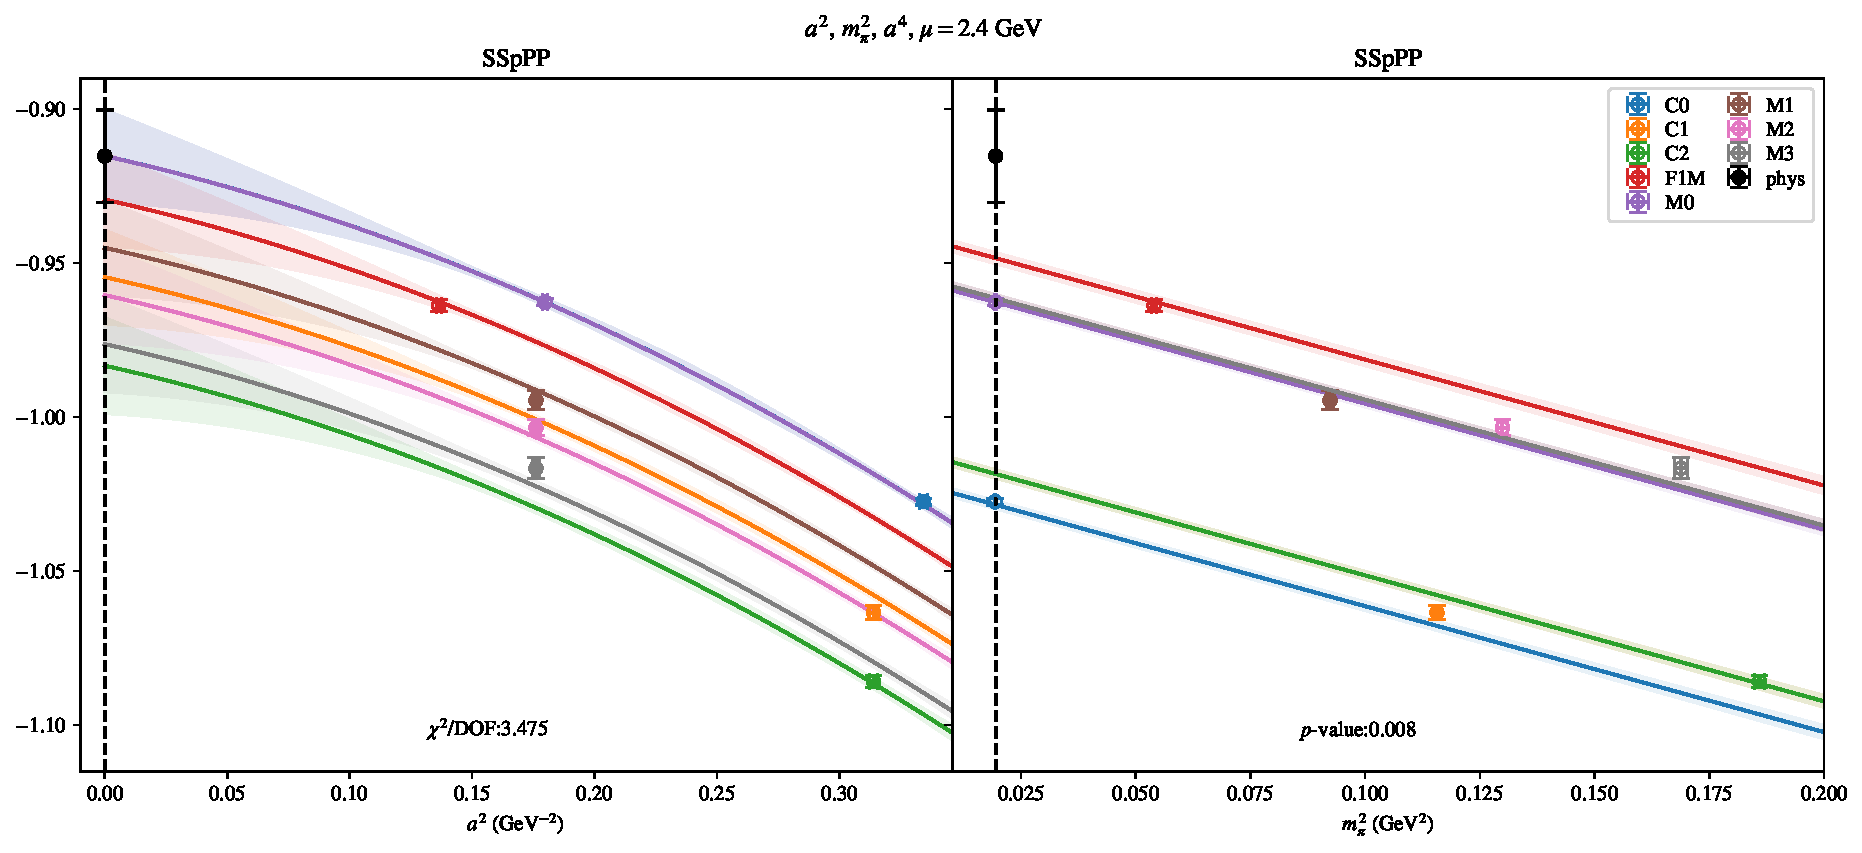
\includepdf[link, pages=-]{VVmAA/SUSY/bag_a2a4m2_24.pdf}
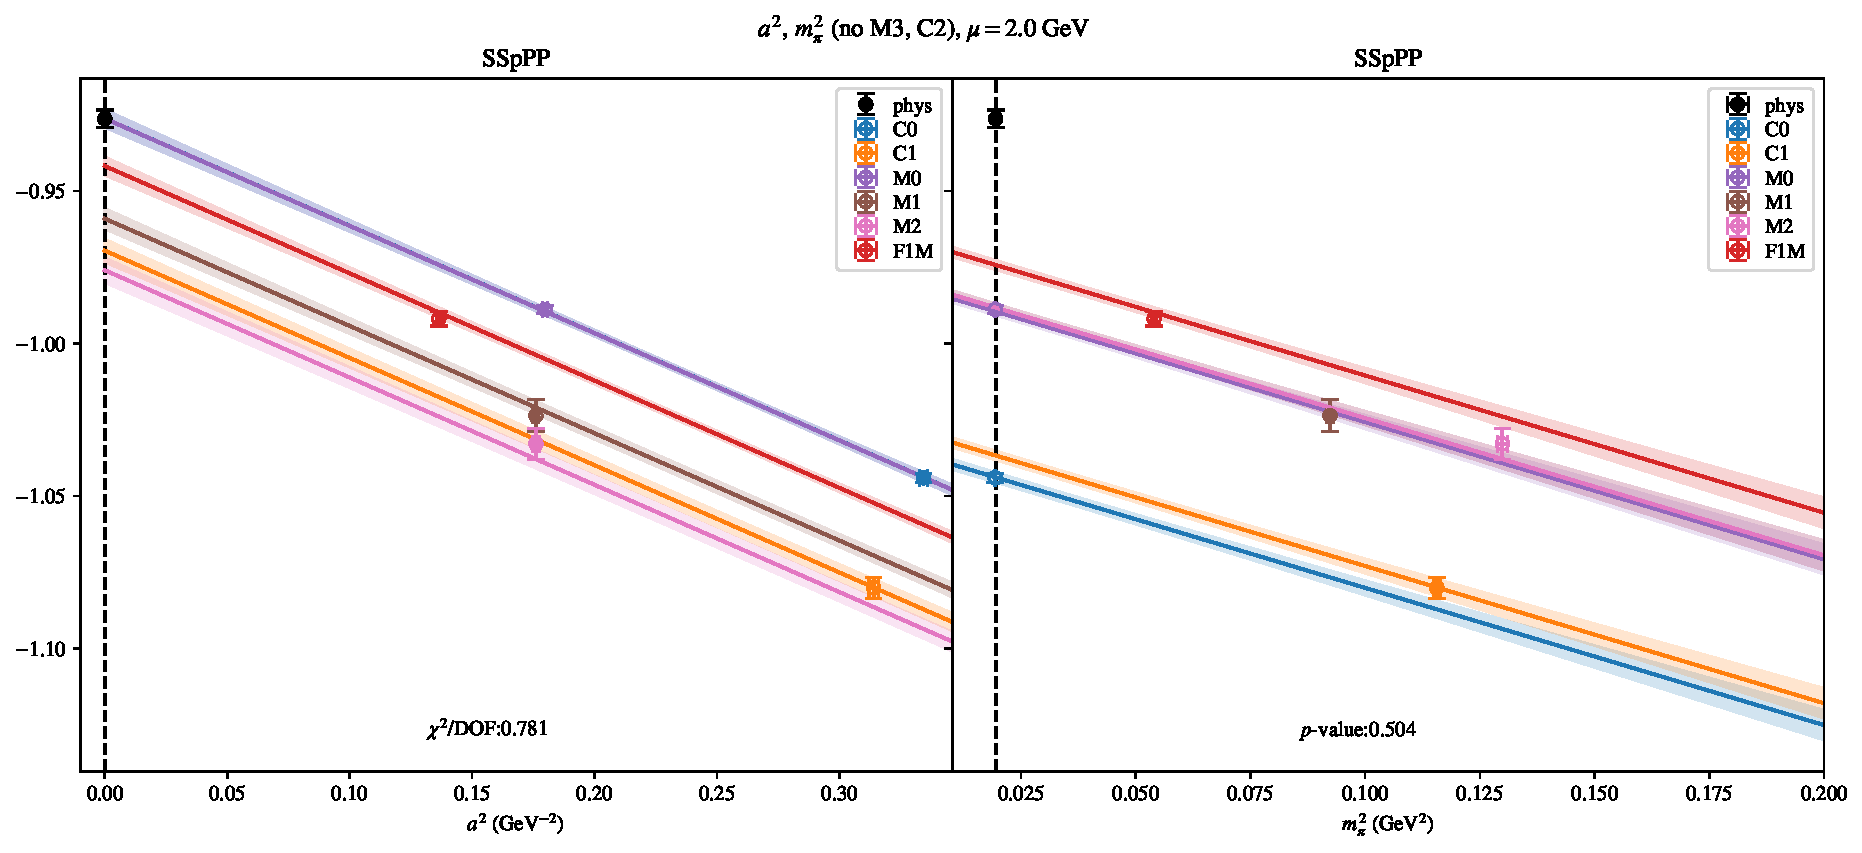
\includepdf[link, pages=-]{VVmAA/SUSY/bag_a2m2mcut_20.pdf}
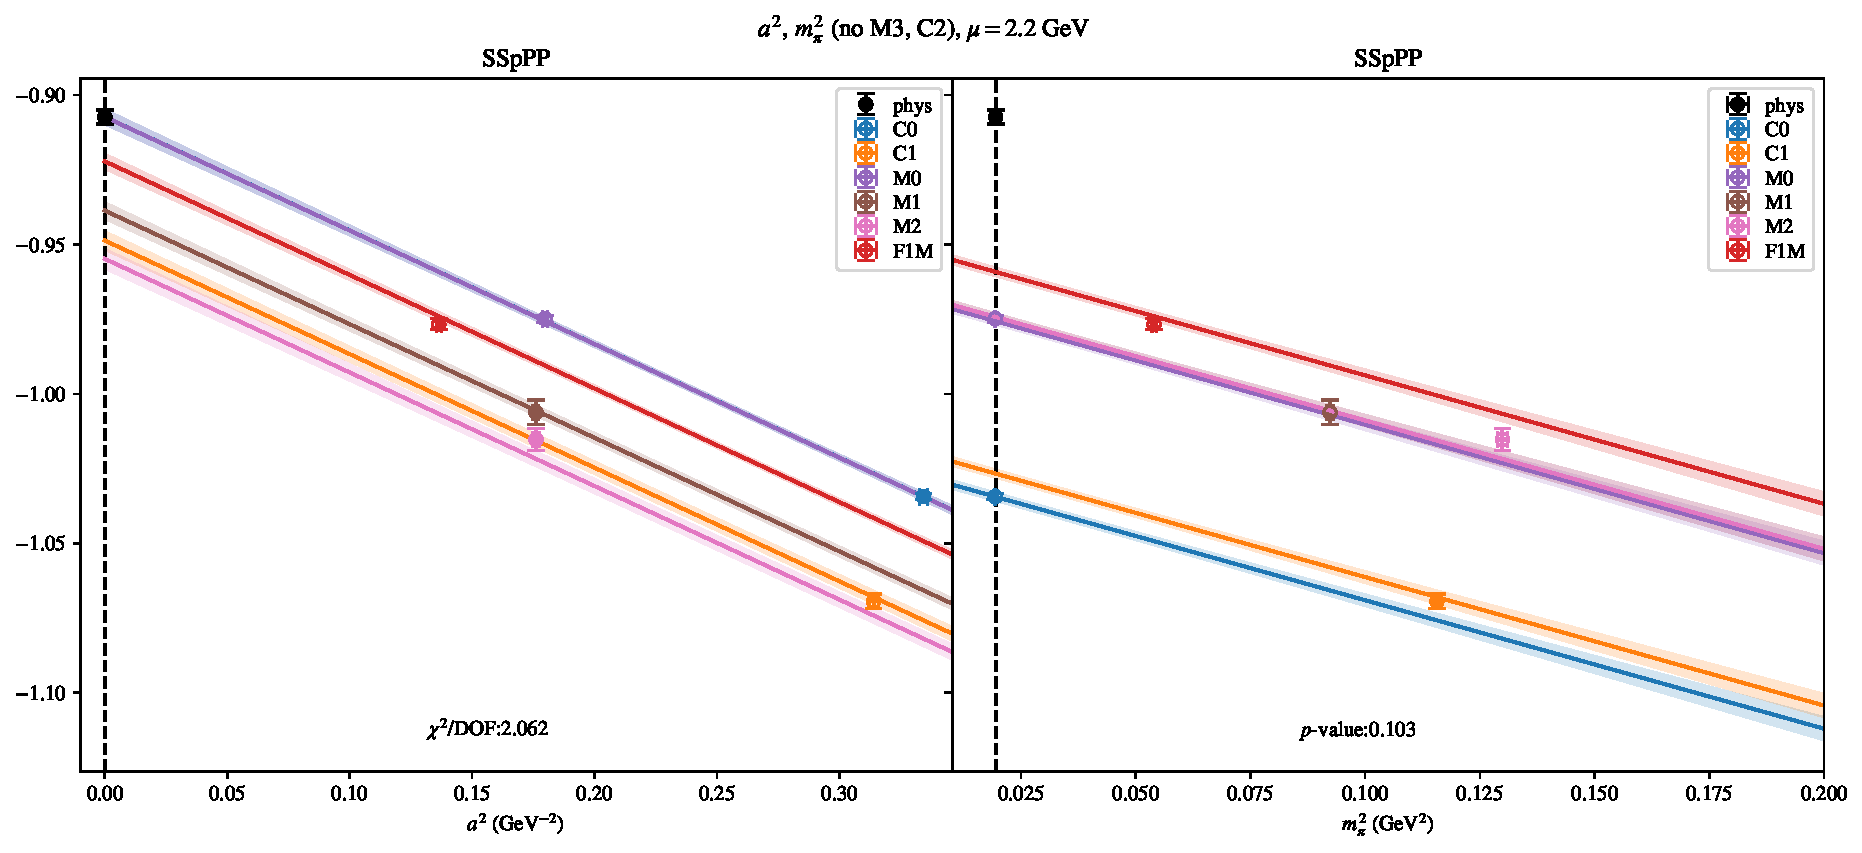
\includepdf[link, pages=-]{VVmAA/SUSY/bag_a2m2mcut_22.pdf}
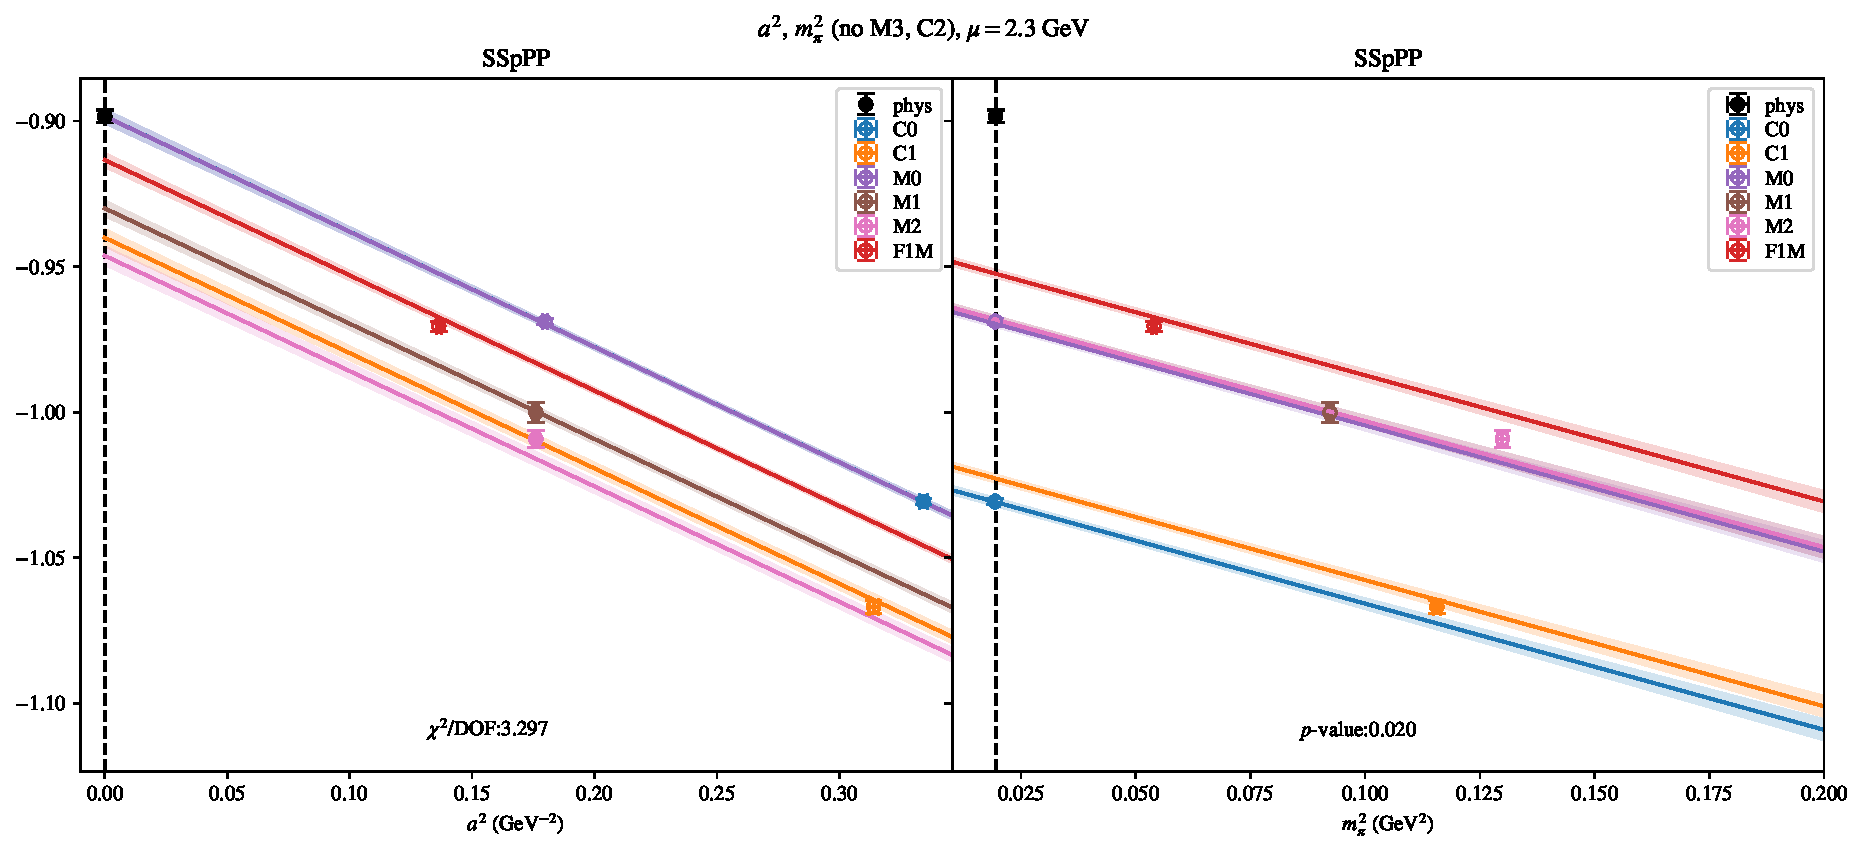
\includepdf[link, pages=-]{VVmAA/SUSY/bag_a2m2mcut_23.pdf}
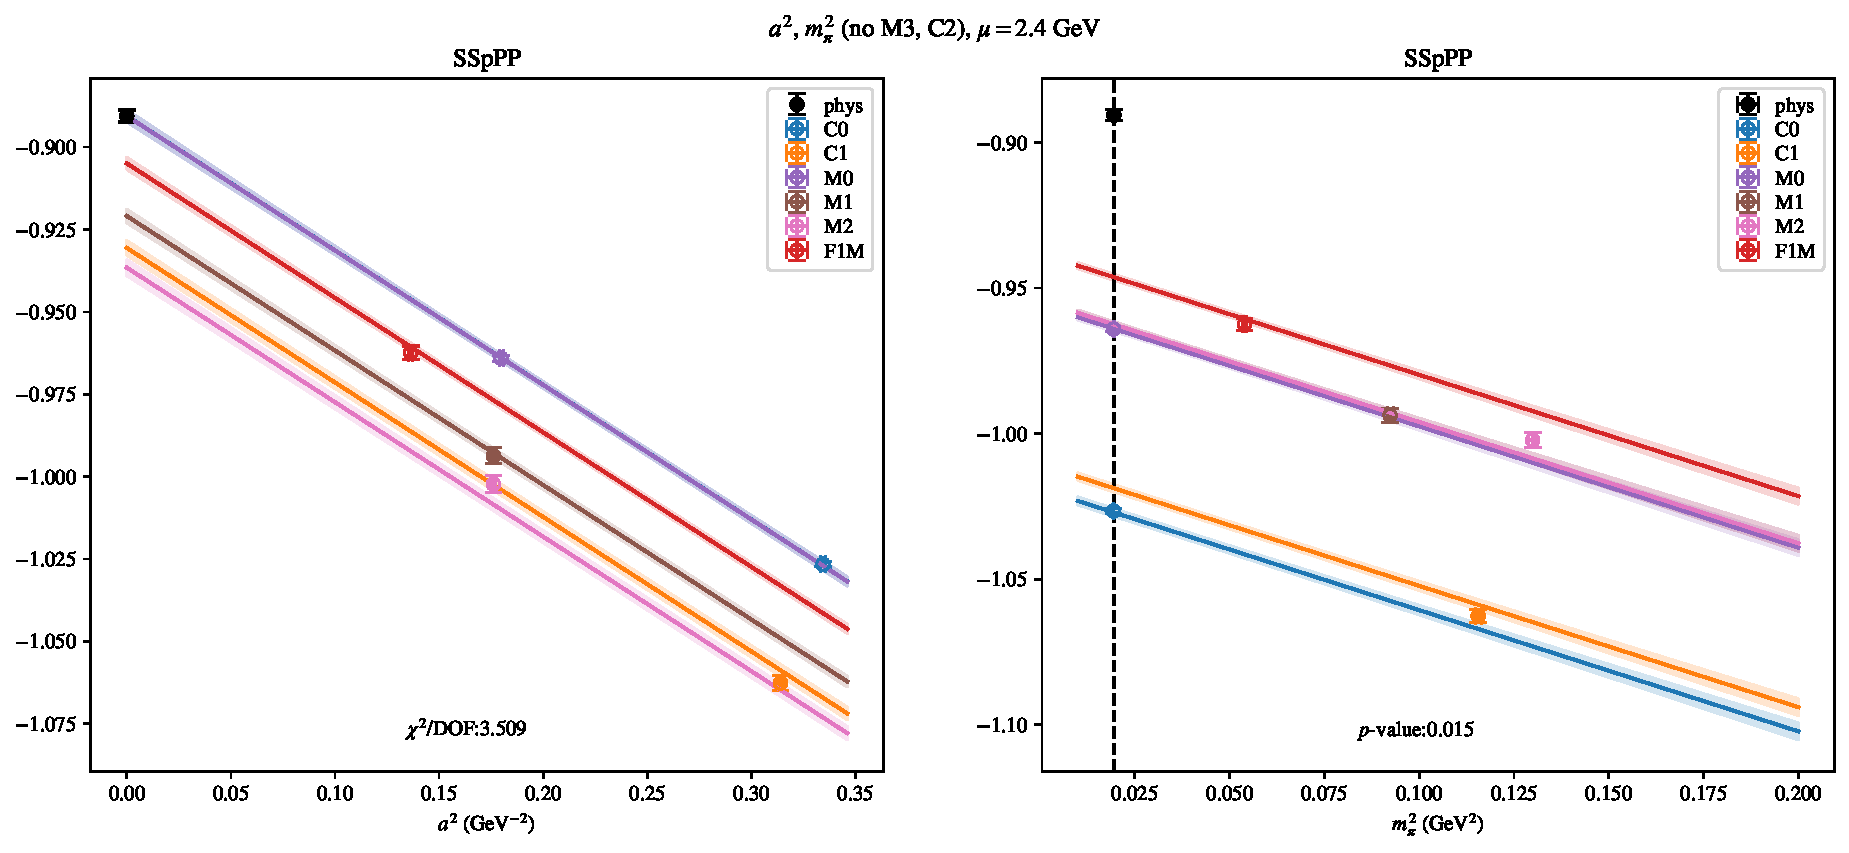
\includepdf[link, pages=-]{VVmAA/SUSY/bag_a2m2mcut_24.pdf}
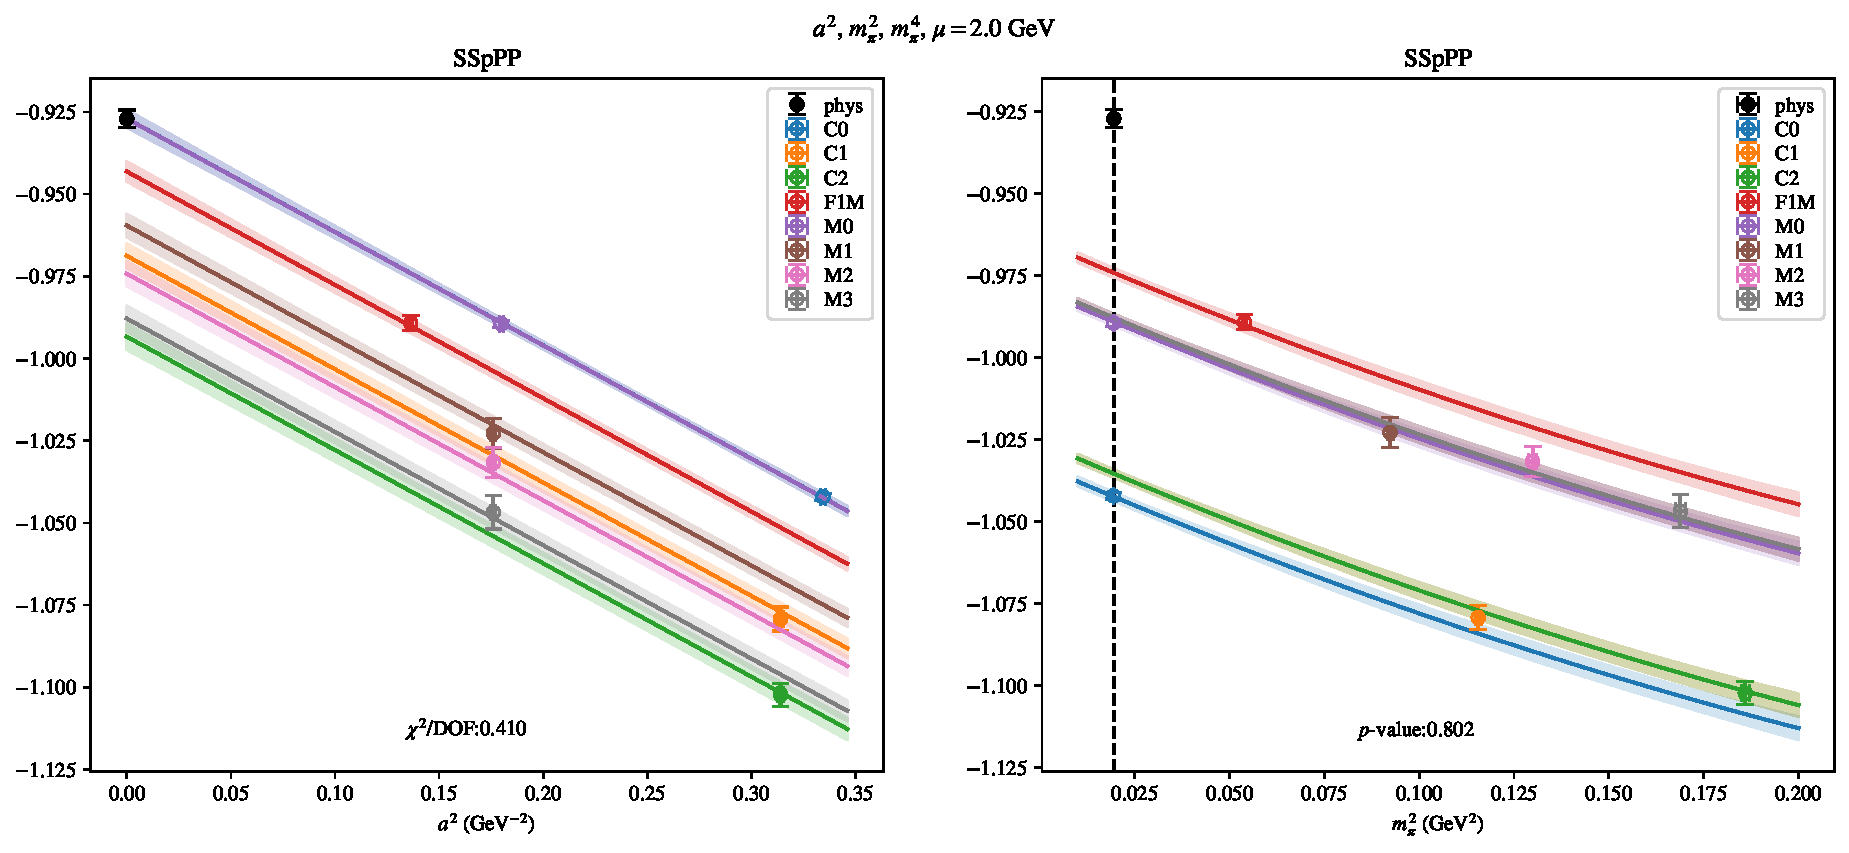
\includepdf[link, pages=-]{VVmAA/SUSY/bag_a2m2m4_20.pdf}
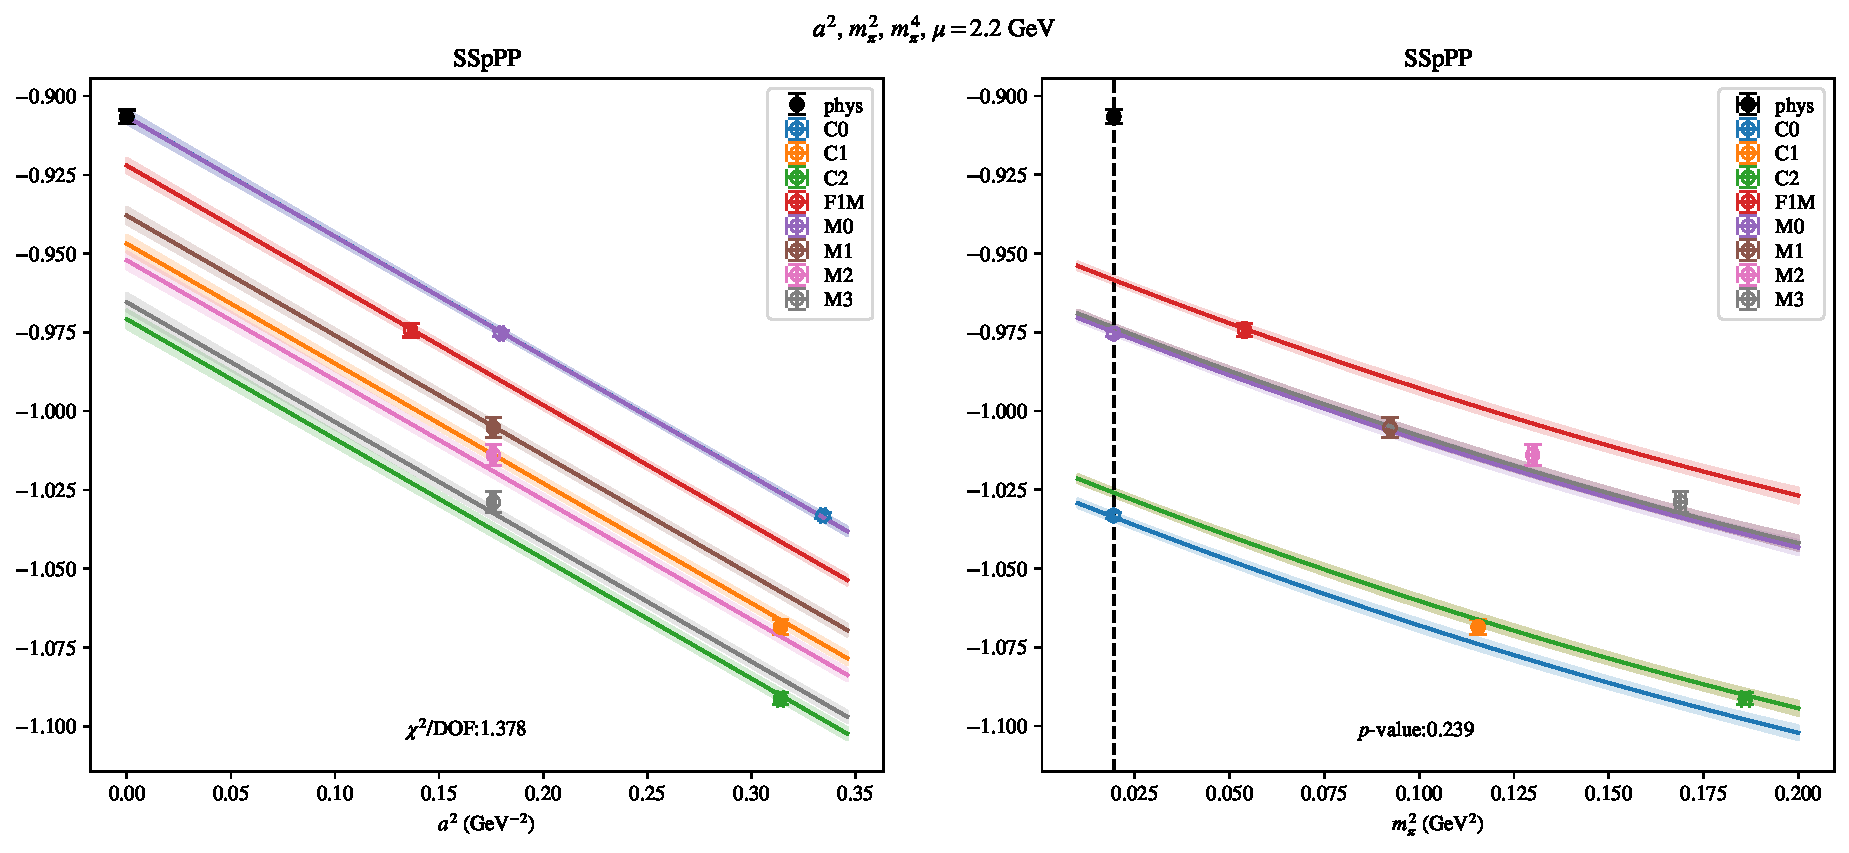
\includepdf[link, pages=-]{VVmAA/SUSY/bag_a2m2m4_22.pdf}
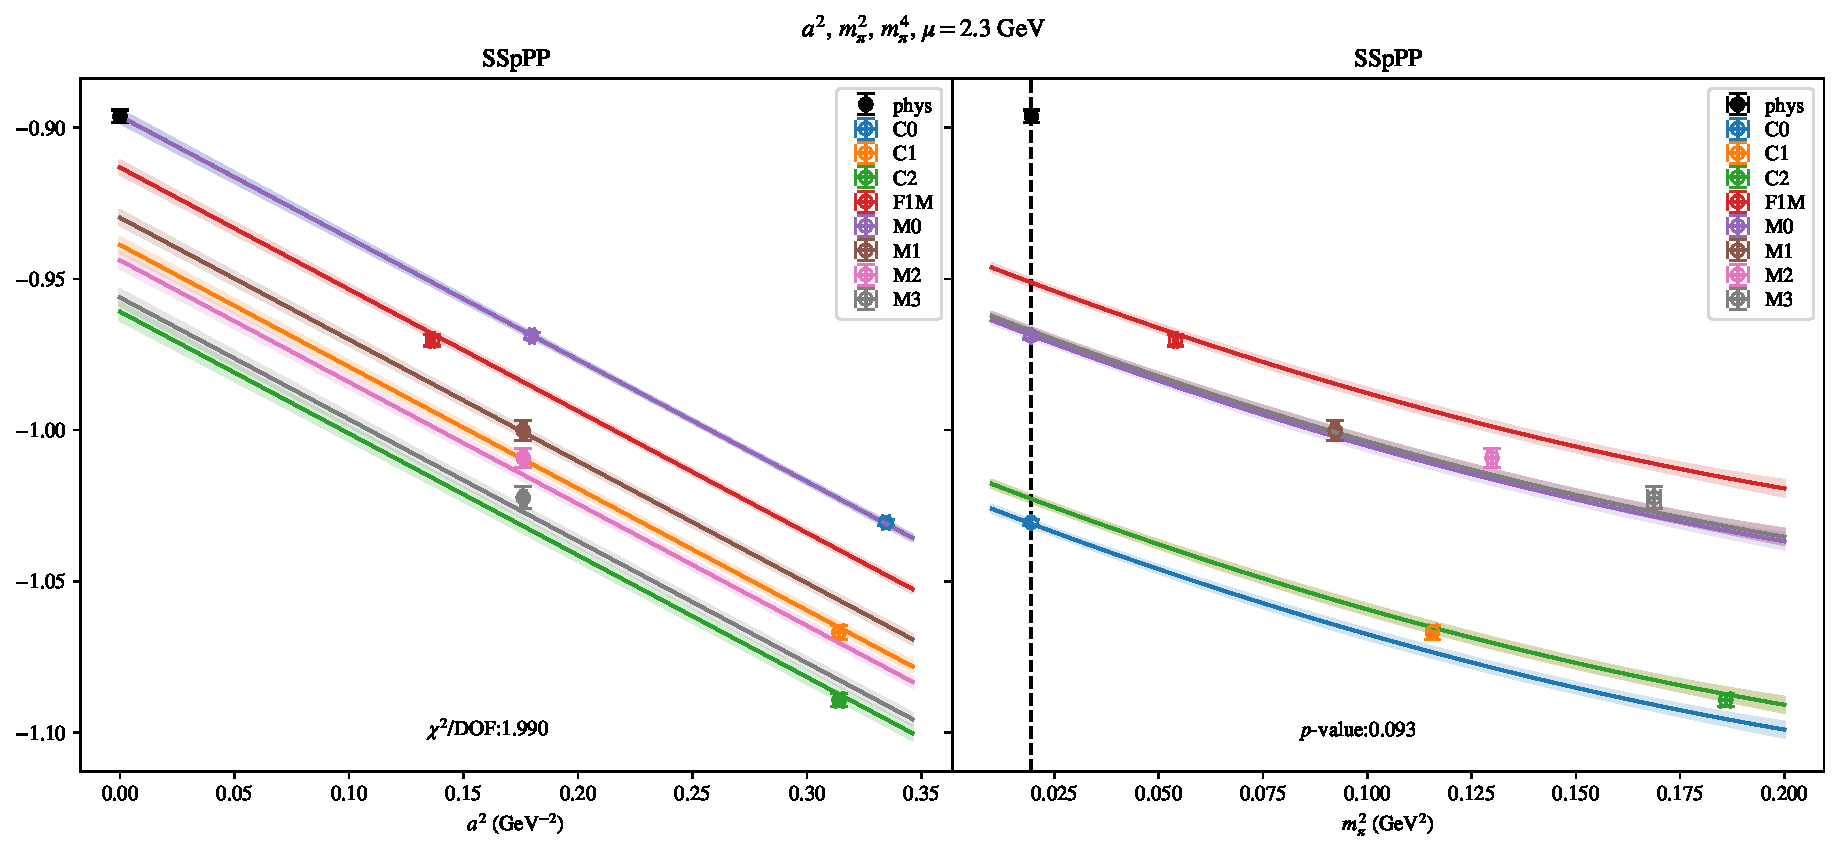
\includepdf[link, pages=-]{VVmAA/SUSY/bag_a2m2m4_23.pdf}
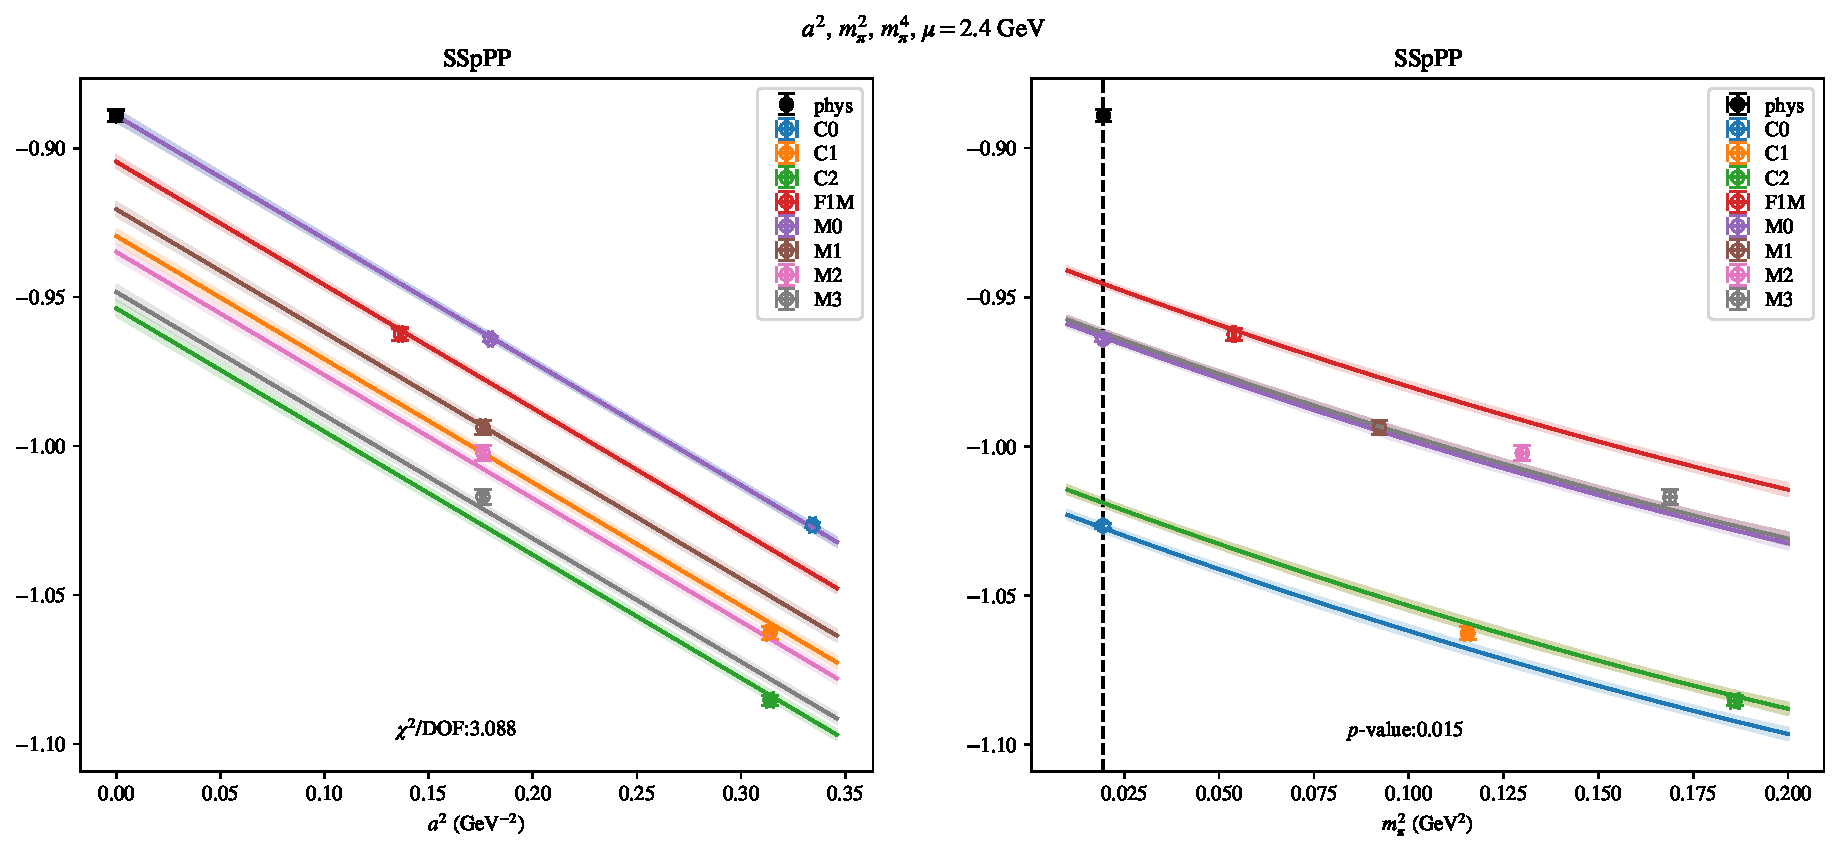
\includepdf[link, pages=-]{VVmAA/SUSY/bag_a2m2m4_24.pdf}
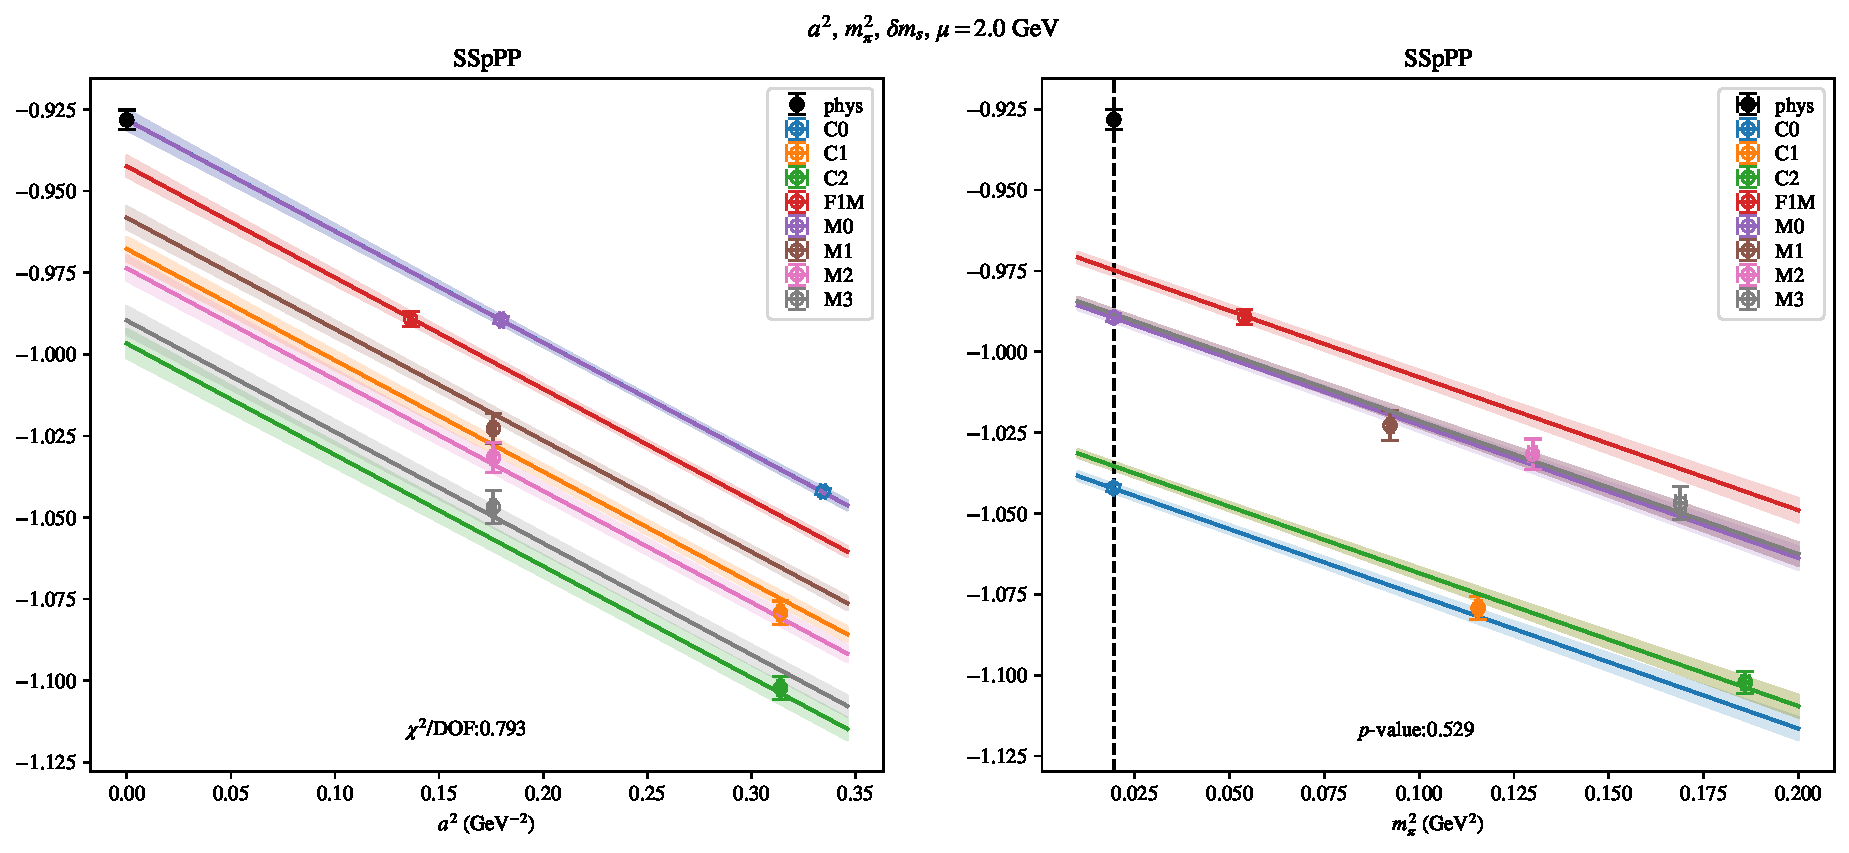
\includepdf[link, pages=-]{VVmAA/SUSY/bag_a2m2delm_20.pdf}
\includepdf[link, pages=-]{VVmAA/SUSY/bag_a2m2delm_22.pdf}
\includepdf[link, pages=-]{VVmAA/SUSY/bag_a2m2delm_23.pdf}
\includepdf[link, pages=-]{VVmAA/SUSY/bag_a2m2delm_24.pdf}
\clearpage
\section{$\mathcal{B}_3$}
\begin{table}[h!]
\begin{center}
\begin{tabular}{|c|c|c|c|c|c|c|}
\hline
$\mu$ (GeV) & $a^2$, $m_\pi^2$& $a^2$, $m_\pi^2$ (no C)& $a^2$, $m_\pi^2$, $a^4$& $a^2$, $m_\pi^2$ (no M3, C2)& $a^2$, $m_\pi^2$, $m_\pi^4$& $a^2$, $m_\pi^2$, $\delta m_s$\\
\hline
2.0& \hyperlink{SSmPP/SUSY/bag_a2m2_20.pdf.1}{\textbf{0.28282(91)}: 0.885 (0.49)} & \hyperlink{SSmPP/SUSY/bag_a2m2noC_20.pdf.1}{\textbf{0.2834(31)}: 1.208 (0.299)} & \hyperlink{SSmPP/SUSY/bag_a2a4m2_20.pdf.1}{\textbf{0.2832(49)}: 1.104 (0.352)} & \hyperlink{SSmPP/SUSY/bag_a2m2mcut_20.pdf.1}{\textbf{0.28251(83)}: 0.671 (0.57)} & \hyperlink{SSmPP/SUSY/bag_a2m2m4_20.pdf.1}{\textbf{0.28226(90)}: 0.444 (0.777)} & \hyperlink{SSmPP/SUSY/bag_a2m2delm_20.pdf.1}{\textbf{0.2828(10)}: 1.106 (0.352)}\\
2.2& \hyperlink{SSmPP/SUSY/bag_a2m2_22.pdf.1}{\textbf{0.27411(73)}: 1.963 (0.081)} & \hyperlink{SSmPP/SUSY/bag_a2m2noC_22.pdf.1}{\textbf{0.2774(29)}: 1.486 (0.226)} & \hyperlink{SSmPP/SUSY/bag_a2a4m2_22.pdf.1}{\textbf{0.2763(46)}: 2.399 (0.048)} & \hyperlink{SSmPP/SUSY/bag_a2m2mcut_22.pdf.1}{\textbf{0.27389(69)}: 1.597 (0.188)} & \hyperlink{SSmPP/SUSY/bag_a2m2m4_22.pdf.1}{\textbf{0.27349(74)}: 1.075 (0.367)} & \hyperlink{SSmPP/SUSY/bag_a2m2delm_22.pdf.1}{\textbf{0.27392(82)}: 2.338 (0.053)}\\
2.3& \hyperlink{SSmPP/SUSY/bag_a2m2_23.pdf.1}{\textbf{0.27016(70)}: 2.789 (0.016)} & \hyperlink{SSmPP/SUSY/bag_a2m2noC_23.pdf.1}{\textbf{0.2746(27)}: 1.94 (0.144)} & \hyperlink{SSmPP/SUSY/bag_a2a4m2_23.pdf.1}{\textbf{0.2733(46)}: 3.367 (0.009)} & \hyperlink{SSmPP/SUSY/bag_a2m2mcut_23.pdf.1}{\textbf{0.27000(66)}: 2.655 (0.047)} & \hyperlink{SSmPP/SUSY/bag_a2m2m4_23.pdf.1}{\textbf{0.26952(71)}: 1.889 (0.109)} & \hyperlink{SSmPP/SUSY/bag_a2m2delm_23.pdf.1}{\textbf{0.26991(76)}: 3.214 (0.012)}\\
2.4& \hyperlink{SSmPP/SUSY/bag_a2m2_24.pdf.1}{\textbf{0.26671(67)}: 3.489 (0.004)} & \hyperlink{SSmPP/SUSY/bag_a2m2noC_24.pdf.1}{\textbf{0.2718(27)}: 2.214 (0.109)} & \hyperlink{SSmPP/SUSY/bag_a2a4m2_24.pdf.1}{\textbf{0.2699(45)}: 4.234 (0.002)} & \hyperlink{SSmPP/SUSY/bag_a2m2mcut_24.pdf.1}{\textbf{0.26661(64)}: 3.517 (0.014)} & \hyperlink{SSmPP/SUSY/bag_a2m2m4_24.pdf.1}{\textbf{0.26607(69)}: 2.727 (0.028)} & \hyperlink{SSmPP/SUSY/bag_a2m2delm_24.pdf.1}{\textbf{0.26644(73)}: 3.989 (0.003)}\\
\hline
\end{tabular}
\caption{Physical point value from chiral and continuum extrapolation at renormalisation scale $\mu$. Entries are \textbf{value(error)}: $\chi^2/\text{DOF}$ ($p$-value).}
\end{center}
\end{table}
\begin{table}[h!]
\begin{center}
\begin{tabular}{|c c|c|c|c|c|c|c|}
\hline
$\mu$ (GeV) &  & $a^2$, $m_\pi^2$& $a^2$, $m_\pi^2$ (no C)& $a^2$, $m_\pi^2$, $a^4$& $a^2$, $m_\pi^2$ (no M3, C2)& $a^2$, $m_\pi^2$, $m_\pi^4$& $a^2$, $m_\pi^2$, $\delta m_s$\\
\hline
\multirow{3}{0.5in}{2.0} & $\alpha$ & 0.1772(35)& 0.174(19)& 0.173(45)& 0.1781(33)& 0.1790(35)& 0.1772(38)\\
 & $\beta$ & 0.00226(11)& 0.00226(19)& 0.00226(11)& 0.00245(15)& 0.00296(32)& 0.00226(11)\\
 & $\gamma$ &  &  & 0.008(90)&  & -0.000068(26)& -0.00001(81)\\
\hline
\multirow{3}{0.5in}{2.2} & $\alpha$ & 0.2022(29)& 0.184(17)& 0.182(42)& 0.2027(28)& 0.2041(29)& 0.2028(31)\\
 & $\beta$ & 0.002182(73)& 0.00209(13)& 0.002188(73)& 0.00237(11)& 0.00291(26)& 0.002192(72)\\
 & $\gamma$ &  &  & 0.040(85)&  & -0.000068(21)& -0.00050(76)\\
\hline
\multirow{3}{0.5in}{2.3} & $\alpha$ & 0.2147(28)& 0.190(16)& 0.186(42)& 0.2151(27)& 0.2168(28)& 0.2156(29)\\
 & $\beta$ & 0.002186(63)& 0.00206(11)& 0.002195(64)& 0.002358(99)& 0.00291(25)& 0.002203(64)\\
 & $\gamma$ &  &  & 0.057(84)&  & -0.000067(21)& -0.00075(72)\\
\hline
\multirow{3}{0.5in}{2.4} & $\alpha$ & 0.2260(27)& 0.198(16)& 0.197(41)& 0.2261(27)& 0.2280(27)& 0.2269(27)\\
 & $\beta$ & 0.002178(57)& 0.002035(98)& 0.002187(59)& 0.002337(92)& 0.00287(24)& 0.002198(59)\\
 & $\gamma$ &  &  & 0.058(83)&  & -0.000064(20)& -0.00086(71)\\
\hline
\end{tabular}
\caption{Fit values of coefficients in $Q = Q_{phys} + \mathbf{\alpha} a^2 + \mathbf{\beta}\left(\frac{m_\pi^2}{f_\pi^2}-\frac{m_{\pi,PDG}^2}{f_\pi^2}\right) + \gamma(\ldots)$}
\end{center}
\end{table}
\includepdf[link, pages=-]{SSmPP/SUSY/bag_a2m2_20.pdf}
\includepdf[link, pages=-]{SSmPP/SUSY/bag_a2m2_22.pdf}
\includepdf[link, pages=-]{SSmPP/SUSY/bag_a2m2_23.pdf}
\includepdf[link, pages=-]{SSmPP/SUSY/bag_a2m2_24.pdf}
\includepdf[link, pages=-]{SSmPP/SUSY/bag_a2m2noC_20.pdf}
\includepdf[link, pages=-]{SSmPP/SUSY/bag_a2m2noC_22.pdf}
\includepdf[link, pages=-]{SSmPP/SUSY/bag_a2m2noC_23.pdf}
\includepdf[link, pages=-]{SSmPP/SUSY/bag_a2m2noC_24.pdf}
\includepdf[link, pages=-]{SSmPP/SUSY/bag_a2a4m2_20.pdf}
\includepdf[link, pages=-]{SSmPP/SUSY/bag_a2a4m2_22.pdf}
\includepdf[link, pages=-]{SSmPP/SUSY/bag_a2a4m2_23.pdf}
\includepdf[link, pages=-]{SSmPP/SUSY/bag_a2a4m2_24.pdf}
\includepdf[link, pages=-]{SSmPP/SUSY/bag_a2m2mcut_20.pdf}
\includepdf[link, pages=-]{SSmPP/SUSY/bag_a2m2mcut_22.pdf}
\includepdf[link, pages=-]{SSmPP/SUSY/bag_a2m2mcut_23.pdf}
\includepdf[link, pages=-]{SSmPP/SUSY/bag_a2m2mcut_24.pdf}
\includepdf[link, pages=-]{SSmPP/SUSY/bag_a2m2m4_20.pdf}
\includepdf[link, pages=-]{SSmPP/SUSY/bag_a2m2m4_22.pdf}
\includepdf[link, pages=-]{SSmPP/SUSY/bag_a2m2m4_23.pdf}
\includepdf[link, pages=-]{SSmPP/SUSY/bag_a2m2m4_24.pdf}
\includepdf[link, pages=-]{SSmPP/SUSY/bag_a2m2delm_20.pdf}
\includepdf[link, pages=-]{SSmPP/SUSY/bag_a2m2delm_22.pdf}
\includepdf[link, pages=-]{SSmPP/SUSY/bag_a2m2delm_23.pdf}
\includepdf[link, pages=-]{SSmPP/SUSY/bag_a2m2delm_24.pdf}
\clearpage
\section{$\mathcal{B}_4$}
\begin{table}[h!]
\begin{center}
\begin{tabular}{|c|c|c|c|c|c|c|}
\hline
$\mu$ (GeV) & $a^2$, $m_\pi^2$& $a^2$, $m_\pi^2$ (no C)& $a^2$, $m_\pi^2$, $a^4$& $a^2$, $m_\pi^2$ (no M3, C2)& $a^2$, $m_\pi^2$, $m_\pi^4$& $a^2$, $m_\pi^2$, $\delta m_s$\\
\hline
2.0& \hyperlink{SSpPP/SUSY/bag_a2m2_20.pdf.1}{\textbf{1.8009(39)}: 14.74 (0.0)} & \hyperlink{SSpPP/SUSY/bag_a2m2noC_20.pdf.1}{\textbf{1.681(14)}: 0.218 (0.804)} & \hyperlink{SSpPP/SUSY/bag_a2a4m2_20.pdf.1}{\textbf{1.608(19)}: 1.029 (0.391)} & \hyperlink{SSpPP/SUSY/bag_a2m2mcut_20.pdf.1}{\textbf{1.8026(35)}: 21.834 (0.0)} & \hyperlink{SSpPP/SUSY/bag_a2m2m4_20.pdf.1}{\textbf{1.8089(38)}: 11.537 (0.0)} & \hyperlink{SSpPP/SUSY/bag_a2m2delm_20.pdf.1}{\textbf{1.8143(45)}: 0.389 (0.817)}\\
2.2& \hyperlink{SSpPP/SUSY/bag_a2m2_22.pdf.1}{\textbf{1.8069(34)}: 14.185 (0.0)} & \hyperlink{SSpPP/SUSY/bag_a2m2noC_22.pdf.1}{\textbf{1.700(13)}: 0.722 (0.486)} & \hyperlink{SSpPP/SUSY/bag_a2a4m2_22.pdf.1}{\textbf{1.635(19)}: 1.347 (0.25)} & \hyperlink{SSpPP/SUSY/bag_a2m2mcut_22.pdf.1}{\textbf{1.8080(31)}: 21.36 (0.0)} & \hyperlink{SSpPP/SUSY/bag_a2m2m4_22.pdf.1}{\textbf{1.8125(33)}: 12.495 (0.0)} & \hyperlink{SSpPP/SUSY/bag_a2m2delm_22.pdf.1}{\textbf{1.8177(38)}: 0.983 (0.415)}\\
2.3& \hyperlink{SSpPP/SUSY/bag_a2m2_23.pdf.1}{\textbf{1.8085(32)}: 13.916 (0.0)} & \hyperlink{SSpPP/SUSY/bag_a2m2noC_23.pdf.1}{\textbf{1.706(12)}: 0.918 (0.399)} & \hyperlink{SSpPP/SUSY/bag_a2a4m2_23.pdf.1}{\textbf{1.641(19)}: 1.196 (0.31)} & \hyperlink{SSpPP/SUSY/bag_a2m2mcut_23.pdf.1}{\textbf{1.8096(30)}: 21.218 (0.0)} & \hyperlink{SSpPP/SUSY/bag_a2m2m4_23.pdf.1}{\textbf{1.8138(32)}: 12.615 (0.0)} & \hyperlink{SSpPP/SUSY/bag_a2m2delm_23.pdf.1}{\textbf{1.8186(36)}: 1.167 (0.323)}\\
2.4& \hyperlink{SSpPP/SUSY/bag_a2m2_24.pdf.1}{\textbf{1.8103(30)}: 13.489 (0.0)} & \hyperlink{SSpPP/SUSY/bag_a2m2noC_24.pdf.1}{\textbf{1.711(12)}: 1.092 (0.335)} & \hyperlink{SSpPP/SUSY/bag_a2a4m2_24.pdf.1}{\textbf{1.649(19)}: 1.368 (0.242)} & \hyperlink{SSpPP/SUSY/bag_a2m2mcut_24.pdf.1}{\textbf{1.8112(29)}: 20.775 (0.0)} & \hyperlink{SSpPP/SUSY/bag_a2m2m4_24.pdf.1}{\textbf{1.8152(30)}: 12.791 (0.0)} & \hyperlink{SSpPP/SUSY/bag_a2m2delm_24.pdf.1}{\textbf{1.8194(33)}: 1.343 (0.251)}\\
\hline
\end{tabular}
\caption{Physical point value from chiral and continuum extrapolation at renormalisation scale $\mu$. Entries are \textbf{value(error)}: $\chi^2/\text{DOF}$ ($p$-value).}
\end{center}
\end{table}
\begin{table}[h!]
\begin{center}
\begin{tabular}{|c c|c|c|c|c|c|c|}
\hline
$\mu$ (GeV) &  & $a^2$, $m_\pi^2$& $a^2$, $m_\pi^2$ (no C)& $a^2$, $m_\pi^2$, $a^4$& $a^2$, $m_\pi^2$ (no M3, C2)& $a^2$, $m_\pi^2$, $m_\pi^4$& $a^2$, $m_\pi^2$, $\delta m_s$\\
\hline
\multirow{3}{0.5in}{2.0} & $\alpha$ & 0.129(14)& 0.830(83)& 1.87(17)& 0.124(13)& 0.103(14)& 0.082(16)\\
 & $\beta$ & -0.00100(47)& -0.00007(92)& -0.00117(47)& -0.00253(70)& -0.0112(14)& -0.00132(47)\\
 & $\gamma$ &  &  & -3.50(36)&  & 0.00097(12)& 0.0311(34)\\
\hline
\multirow{3}{0.5in}{2.2} & $\alpha$ & 0.135(12)& 0.759(76)& 1.68(17)& 0.132(11)& 0.117(12)& 0.096(13)\\
 & $\beta$ & -0.00111(31)& -0.00078(70)& -0.00160(31)& -0.00216(52)& -0.0078(12)& -0.00162(31)\\
 & $\gamma$ &  &  & -3.11(35)&  & 0.00061(10)& 0.0276(32)\\
\hline
\multirow{3}{0.5in}{2.3} & $\alpha$ & 0.140(12)& 0.739(75)& 1.65(17)& 0.137(11)& 0.123(11)& 0.104(13)\\
 & $\beta$ & -0.00086(29)& -0.00073(58)& -0.00136(29)& -0.00178(49)& -0.0069(12)& -0.00140(29)\\
 & $\gamma$ &  &  & -3.04(36)&  & 0.00056(10)& 0.0265(33)\\
\hline
\multirow{3}{0.5in}{2.4} & $\alpha$ & 0.142(11)& 0.723(74)& 1.60(17)& 0.140(11)& 0.126(11)& 0.109(12)\\
 & $\beta$ & -0.00075(26)& -0.00065(50)& -0.00126(26)& -0.00150(45)& -0.0059(11)& -0.00130(26)\\
 & $\gamma$ &  &  & -2.93(35)&  & 0.00047(10)& 0.0255(32)\\
\hline
\end{tabular}
\caption{Fit values of coefficients in $Q = Q_{phys} + \mathbf{\alpha} a^2 + \mathbf{\beta}\left(\frac{m_\pi^2}{f_\pi^2}-\frac{m_{\pi,PDG}^2}{f_\pi^2}\right) + \gamma(\ldots)$}
\end{center}
\end{table}
\includepdf[link, pages=-]{SSpPP/SUSY/bag_a2m2_20.pdf}
\includepdf[link, pages=-]{SSpPP/SUSY/bag_a2m2_22.pdf}
\includepdf[link, pages=-]{SSpPP/SUSY/bag_a2m2_23.pdf}
\includepdf[link, pages=-]{SSpPP/SUSY/bag_a2m2_24.pdf}
\includepdf[link, pages=-]{SSpPP/SUSY/bag_a2m2noC_20.pdf}
\includepdf[link, pages=-]{SSpPP/SUSY/bag_a2m2noC_22.pdf}
\includepdf[link, pages=-]{SSpPP/SUSY/bag_a2m2noC_23.pdf}
\includepdf[link, pages=-]{SSpPP/SUSY/bag_a2m2noC_24.pdf}
\includepdf[link, pages=-]{SSpPP/SUSY/bag_a2a4m2_20.pdf}
\includepdf[link, pages=-]{SSpPP/SUSY/bag_a2a4m2_22.pdf}
\includepdf[link, pages=-]{SSpPP/SUSY/bag_a2a4m2_23.pdf}
\includepdf[link, pages=-]{SSpPP/SUSY/bag_a2a4m2_24.pdf}
\includepdf[link, pages=-]{SSpPP/SUSY/bag_a2m2mcut_20.pdf}
\includepdf[link, pages=-]{SSpPP/SUSY/bag_a2m2mcut_22.pdf}
\includepdf[link, pages=-]{SSpPP/SUSY/bag_a2m2mcut_23.pdf}
\includepdf[link, pages=-]{SSpPP/SUSY/bag_a2m2mcut_24.pdf}
\includepdf[link, pages=-]{SSpPP/SUSY/bag_a2m2m4_20.pdf}
\includepdf[link, pages=-]{SSpPP/SUSY/bag_a2m2m4_22.pdf}
\includepdf[link, pages=-]{SSpPP/SUSY/bag_a2m2m4_23.pdf}
\includepdf[link, pages=-]{SSpPP/SUSY/bag_a2m2m4_24.pdf}
\includepdf[link, pages=-]{SSpPP/SUSY/bag_a2m2delm_20.pdf}
\includepdf[link, pages=-]{SSpPP/SUSY/bag_a2m2delm_22.pdf}
\includepdf[link, pages=-]{SSpPP/SUSY/bag_a2m2delm_23.pdf}
\includepdf[link, pages=-]{SSpPP/SUSY/bag_a2m2delm_24.pdf}
\clearpage
\section{$\mathcal{B}_5$}
\begin{table}[h!]
\begin{center}
\begin{tabular}{|c|c|c|c|c|c|c|}
\hline
$\mu$ (GeV) & $a^2$, $m_\pi^2$& $a^2$, $m_\pi^2$ (no C)& $a^2$, $m_\pi^2$, $a^4$& $a^2$, $m_\pi^2$ (no M3, C2)& $a^2$, $m_\pi^2$, $m_\pi^4$& $a^2$, $m_\pi^2$, $\delta m_s$\\
\hline
2.0& \hyperlink{TT/SUSY/bag_a2m2_20.pdf.1}{\textbf{0.4959(11)}: 10.034 (0.0)} & \hyperlink{TT/SUSY/bag_a2m2noC_20.pdf.1}{\textbf{0.4630(47)}: 0.477 (0.621)} & \hyperlink{TT/SUSY/bag_a2a4m2_20.pdf.1}{\textbf{0.4444(65)}: 1.091 (0.359)} & \hyperlink{TT/SUSY/bag_a2m2mcut_20.pdf.1}{\textbf{0.4963(10)}: 14.614 (0.0)} & \hyperlink{TT/SUSY/bag_a2m2m4_20.pdf.1}{\textbf{0.4974(11)}: 8.074 (0.0)} & \hyperlink{TT/SUSY/bag_a2m2delm_20.pdf.1}{\textbf{0.4982(12)}: 0.62 (0.649)}\\
2.2& \hyperlink{TT/SUSY/bag_a2m2_22.pdf.1}{\textbf{0.5030(10)}: 8.915 (0.0)} & \hyperlink{TT/SUSY/bag_a2m2noC_22.pdf.1}{\textbf{0.4744(44)}: 1.253 (0.286)} & \hyperlink{TT/SUSY/bag_a2a4m2_22.pdf.1}{\textbf{0.4576(66)}: 1.284 (0.274)} & \hyperlink{TT/SUSY/bag_a2m2mcut_22.pdf.1}{\textbf{0.50329(95)}: 12.745 (0.0)} & \hyperlink{TT/SUSY/bag_a2m2m4_22.pdf.1}{\textbf{0.50405(98)}: 7.225 (0.0)} & \hyperlink{TT/SUSY/bag_a2m2delm_22.pdf.1}{\textbf{0.5046(10)}: 1.455 (0.213)}\\
2.3& \hyperlink{TT/SUSY/bag_a2m2_23.pdf.1}{\textbf{0.50597(93)}: 9.373 (0.0)} & \hyperlink{TT/SUSY/bag_a2m2noC_23.pdf.1}{\textbf{0.4781(44)}: 1.66 (0.19)} & \hyperlink{TT/SUSY/bag_a2a4m2_23.pdf.1}{\textbf{0.4610(65)}: 1.321 (0.259)} & \hyperlink{TT/SUSY/bag_a2m2mcut_23.pdf.1}{\textbf{0.50627(86)}: 13.608 (0.0)} & \hyperlink{TT/SUSY/bag_a2m2m4_23.pdf.1}{\textbf{0.50698(89)}: 7.826 (0.0)} & \hyperlink{TT/SUSY/bag_a2m2delm_23.pdf.1}{\textbf{0.50739(96)}: 1.86 (0.114)}\\
2.4& \hyperlink{TT/SUSY/bag_a2m2_24.pdf.1}{\textbf{0.50838(87)}: 9.097 (0.0)} & \hyperlink{TT/SUSY/bag_a2m2noC_24.pdf.1}{\textbf{0.4817(43)}: 1.942 (0.143)} & \hyperlink{TT/SUSY/bag_a2a4m2_24.pdf.1}{\textbf{0.4659(64)}: 1.575 (0.178)} & \hyperlink{TT/SUSY/bag_a2m2mcut_24.pdf.1}{\textbf{0.50865(82)}: 13.168 (0.0)} & \hyperlink{TT/SUSY/bag_a2m2m4_24.pdf.1}{\textbf{0.50933(84)}: 7.737 (0.0)} & \hyperlink{TT/SUSY/bag_a2m2delm_24.pdf.1}{\textbf{0.50963(90)}: 2.072 (0.082)}\\
\hline
\end{tabular}
\caption{Physical point value from chiral and continuum extrapolation at renormalisation scale $\mu$. Entries are \textbf{value(error)}: $\chi^2/\text{DOF}$ ($p$-value).}
\end{center}
\end{table}
\begin{table}[h!]
\begin{center}
\begin{tabular}{|c c|c|c|c|c|c|c|}
\hline
$\mu$ (GeV) &  & $a^2$, $m_\pi^2$& $a^2$, $m_\pi^2$ (no C)& $a^2$, $m_\pi^2$, $a^4$& $a^2$, $m_\pi^2$ (no M3, C2)& $a^2$, $m_\pi^2$, $m_\pi^4$& $a^2$, $m_\pi^2$, $\delta m_s$\\
\hline
\multirow{3}{0.5in}{2.0} & $\alpha$ & -0.0898(40)& 0.101(27)& 0.369(58)& -0.0907(37)& -0.0946(39)& -0.0979(43)\\
 & $\beta$ & 0.00081(13)& 0.00101(26)& 0.00073(13)& 0.00043(19)& -0.00159(42)& 0.00069(13)\\
 & $\gamma$ &  &  & -0.91(11)&  & 0.000227(34)& 0.0082(11)\\
\hline
\multirow{3}{0.5in}{2.2} & $\alpha$ & -0.1123(36)& 0.052(25)& 0.290(58)& -0.1131(33)& -0.1157(34)& -0.1182(37)\\
 & $\beta$ & 0.000672(94)& 0.00069(21)& 0.000540(95)& 0.00036(14)& -0.00107(37)& 0.000533(95)\\
 & $\gamma$ &  &  & -0.80(11)&  & 0.000162(31)& 0.0071(10)\\
\hline
\multirow{3}{0.5in}{2.3} & $\alpha$ & -0.1236(32)& 0.037(25)& 0.275(57)& -0.1244(30)& -0.1268(31)& -0.1288(34)\\
 & $\beta$ & 0.000729(88)& 0.00071(17)& 0.000605(89)& 0.00045(13)& -0.00087(35)& 0.000585(89)\\
 & $\gamma$ &  &  & -0.79(11)&  & 0.000148(30)& 0.0069(10)\\
\hline
\multirow{3}{0.5in}{2.4} & $\alpha$ & -0.1342(31)& 0.019(24)& 0.242(56)& -0.1349(29)& -0.1372(30)& -0.1389(32)\\
 & $\beta$ & 0.000724(79)& 0.00072(14)& 0.000604(81)& 0.00048(12)& -0.00070(33)& 0.000581(81)\\
 & $\gamma$ &  &  & -0.75(11)&  & 0.000132(28)& 0.0065(10)\\
\hline
\end{tabular}
\caption{Fit values of coefficients in $Q = Q_{phys} + \mathbf{\alpha} a^2 + \mathbf{\beta}\left(\frac{m_\pi^2}{f_\pi^2}-\frac{m_{\pi,PDG}^2}{f_\pi^2}\right) + \gamma(\ldots)$}
\end{center}
\end{table}
\includepdf[link, pages=-]{TT/SUSY/bag_a2m2_20.pdf}
\includepdf[link, pages=-]{TT/SUSY/bag_a2m2_22.pdf}
\includepdf[link, pages=-]{TT/SUSY/bag_a2m2_23.pdf}
\includepdf[link, pages=-]{TT/SUSY/bag_a2m2_24.pdf}
\includepdf[link, pages=-]{TT/SUSY/bag_a2m2noC_20.pdf}
\includepdf[link, pages=-]{TT/SUSY/bag_a2m2noC_22.pdf}
\includepdf[link, pages=-]{TT/SUSY/bag_a2m2noC_23.pdf}
\includepdf[link, pages=-]{TT/SUSY/bag_a2m2noC_24.pdf}
\includepdf[link, pages=-]{TT/SUSY/bag_a2a4m2_20.pdf}
\includepdf[link, pages=-]{TT/SUSY/bag_a2a4m2_22.pdf}
\includepdf[link, pages=-]{TT/SUSY/bag_a2a4m2_23.pdf}
\includepdf[link, pages=-]{TT/SUSY/bag_a2a4m2_24.pdf}
\includepdf[link, pages=-]{TT/SUSY/bag_a2m2mcut_20.pdf}
\includepdf[link, pages=-]{TT/SUSY/bag_a2m2mcut_22.pdf}
\includepdf[link, pages=-]{TT/SUSY/bag_a2m2mcut_23.pdf}
\includepdf[link, pages=-]{TT/SUSY/bag_a2m2mcut_24.pdf}
\includepdf[link, pages=-]{TT/SUSY/bag_a2m2m4_20.pdf}
\includepdf[link, pages=-]{TT/SUSY/bag_a2m2m4_22.pdf}
\includepdf[link, pages=-]{TT/SUSY/bag_a2m2m4_23.pdf}
\includepdf[link, pages=-]{TT/SUSY/bag_a2m2m4_24.pdf}
\includepdf[link, pages=-]{TT/SUSY/bag_a2m2delm_20.pdf}
\includepdf[link, pages=-]{TT/SUSY/bag_a2m2delm_22.pdf}
\includepdf[link, pages=-]{TT/SUSY/bag_a2m2delm_23.pdf}
\includepdf[link, pages=-]{TT/SUSY/bag_a2m2delm_24.pdf}
\clearpage
\end{document}